To reconstruct all the simulated particles we start with the final state particles and go backwards through the reaction chain.

\section{Final state particle}
	The selected final state particle are protons, antiproton, \piminus, \piplus, \kminus and \kplus mesons.
	For the reconstruction of these final state particles I used an ideal tracking. 
	To make the selection a bit more realistic only particles with more than 3 hits in any inner tracking detector (MVD, STT and GEM)
	are selected.
	The selection criterion is chosen because three hits are defining a cirlce.
	A fourth hit point is than a validation of the track hypothesis.\\
	The particle identification (PID) is also ideal. 
	The selection criterion is set to 'best'.\\
	\vspace{11pt} 
	The reconstruction  efficieny for the final state particle is shown in table \ref{tab:finalstate_recoeff} and figure \ref{fig:finalstate_recoeff}.
	
	\begin{table}
		\centering
		\caption{reco efficiency and momentum resolution for \pbarpSystem $\rightarrow$ \excitedcascade \anticascade}
		\label{tab:finalstate_recoeff}
		\begin{tabular}{lll}
			\hline
			final state & N/$\%$ & $\frac{\sigma p}{p}/\%$ \\
			\hline
			\hline
			\piminus & 83.48 & 1.53\\
			\piplusone(\anticascade) &  80.93& 1.38 \\
			\piplustwo(\alam) &  83.07& 1.49\\
			\kminus&  78.59& 1.58\\
			p &  84.39& 1.61\\
			\antiproton & 78.25 & 1.61\\\hline
			 
		\end{tabular}
	\end{table}
	
	Table \ref{tab:finalstate_recoeff_cc} shows the reconstruction efficiency for the c.c. channel.
	
	\begin{table}
		\centering
		\caption{reco efficiency and momentum resolution for \pbarpSystem $\rightarrow$ \excitedanticascade \cascade}
		\label{tab:finalstate_recoeff_cc}
		\begin{tabular}{lll}
			\hline
			final state & N/$\%$ & $\frac{\sigma p}{p}/\%$ \\
			\hline
			\hline
			\piplus &  82.9625&   1.54131\\
			\piminusone(\cascade) & 80.395&   1.37697  \\
			\piminustwo(\lam) &  82.6867&   1.48918\\
			\kplus& 83.2709&   1.57882 \\
			p &  80.7079&   1.55197\\
			\antiproton &  80.9253&   1.60091\\\hline
			 
		\end{tabular}
	\end{table}
	
	\begin{figure}
	
		\centering
		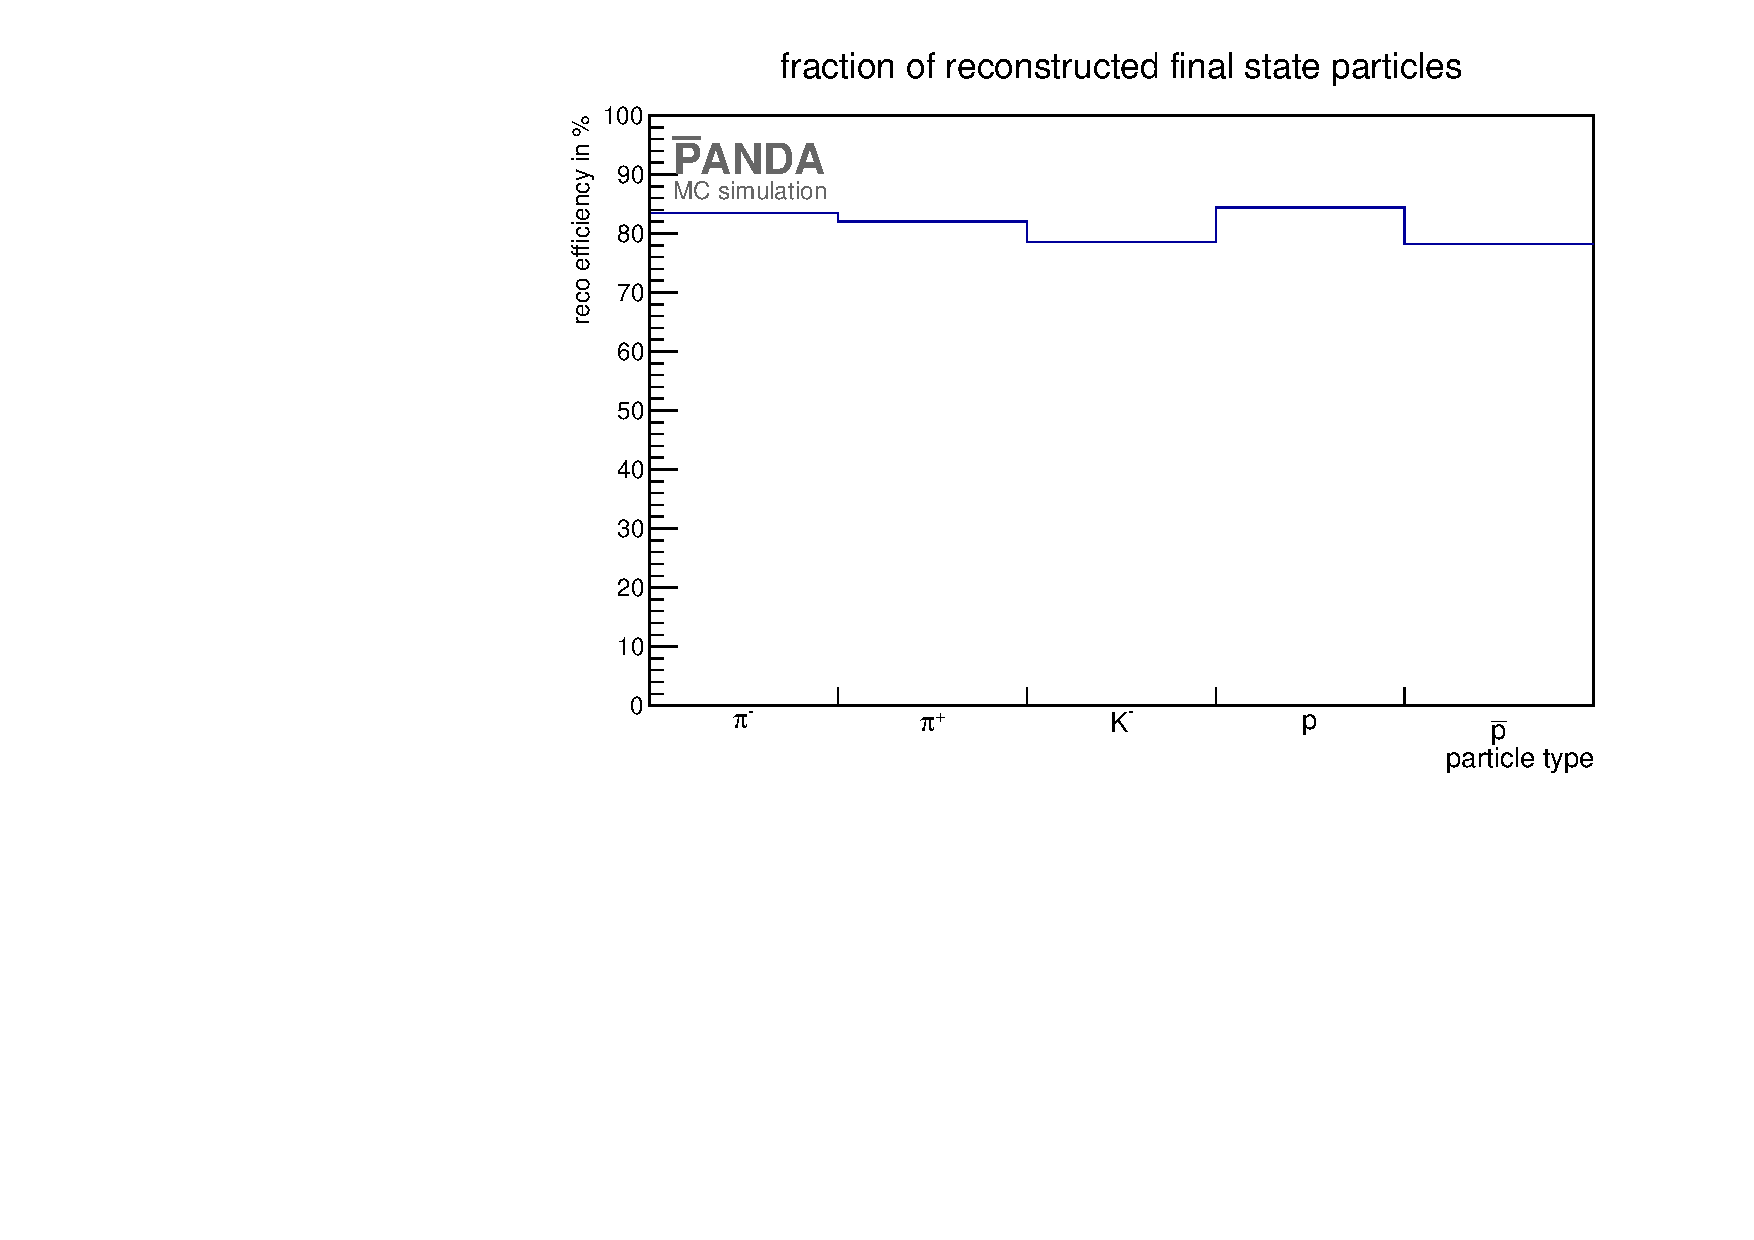
\includegraphics[width=0.8\textwidth]{./plots/finalstate/reco_efficiency.pdf}
		\caption{Reconstruction efficiency for final state particles. The x axis shows the particle type. 
				On the y axis is shown the fraction of reconstructed particles, like it is shown in table \ref{tab:finalstate_recoeff}}
		\label{fig:finalstate_recoeff}
	
	\end{figure}
	

	
\section{Reconstruction of $\boldmath{\Lambda}^0$ and $\boldmath{\bar{\Lambda}^0}$}
	\subsection*{Selection}
		For the reconstruction of 
		
		\begin{itemize}
			\item \lam a proton and a \piminus meson are combined and
			\item for the reconstruction of \alam a \antiproton and a \piplus are combined.
		\end{itemize}
		 
		After the combination of the daughter particles a mass window cut is performed.
		Only those particles are chosen which have a mass within $0.3$\massunit.
		
		
		A vertex constraint fit with the PndKinVertexFitter is performed on the selected particle.
		This means that the tracks of the daughter particles are fitted to a common vertex point.  
		The \chisq and \chisq-Probability distiribution of the vertex fit for \lam is shown in figure \ref{fig:lambda_chi2}.
		
		\begin{figure}
			\centering
				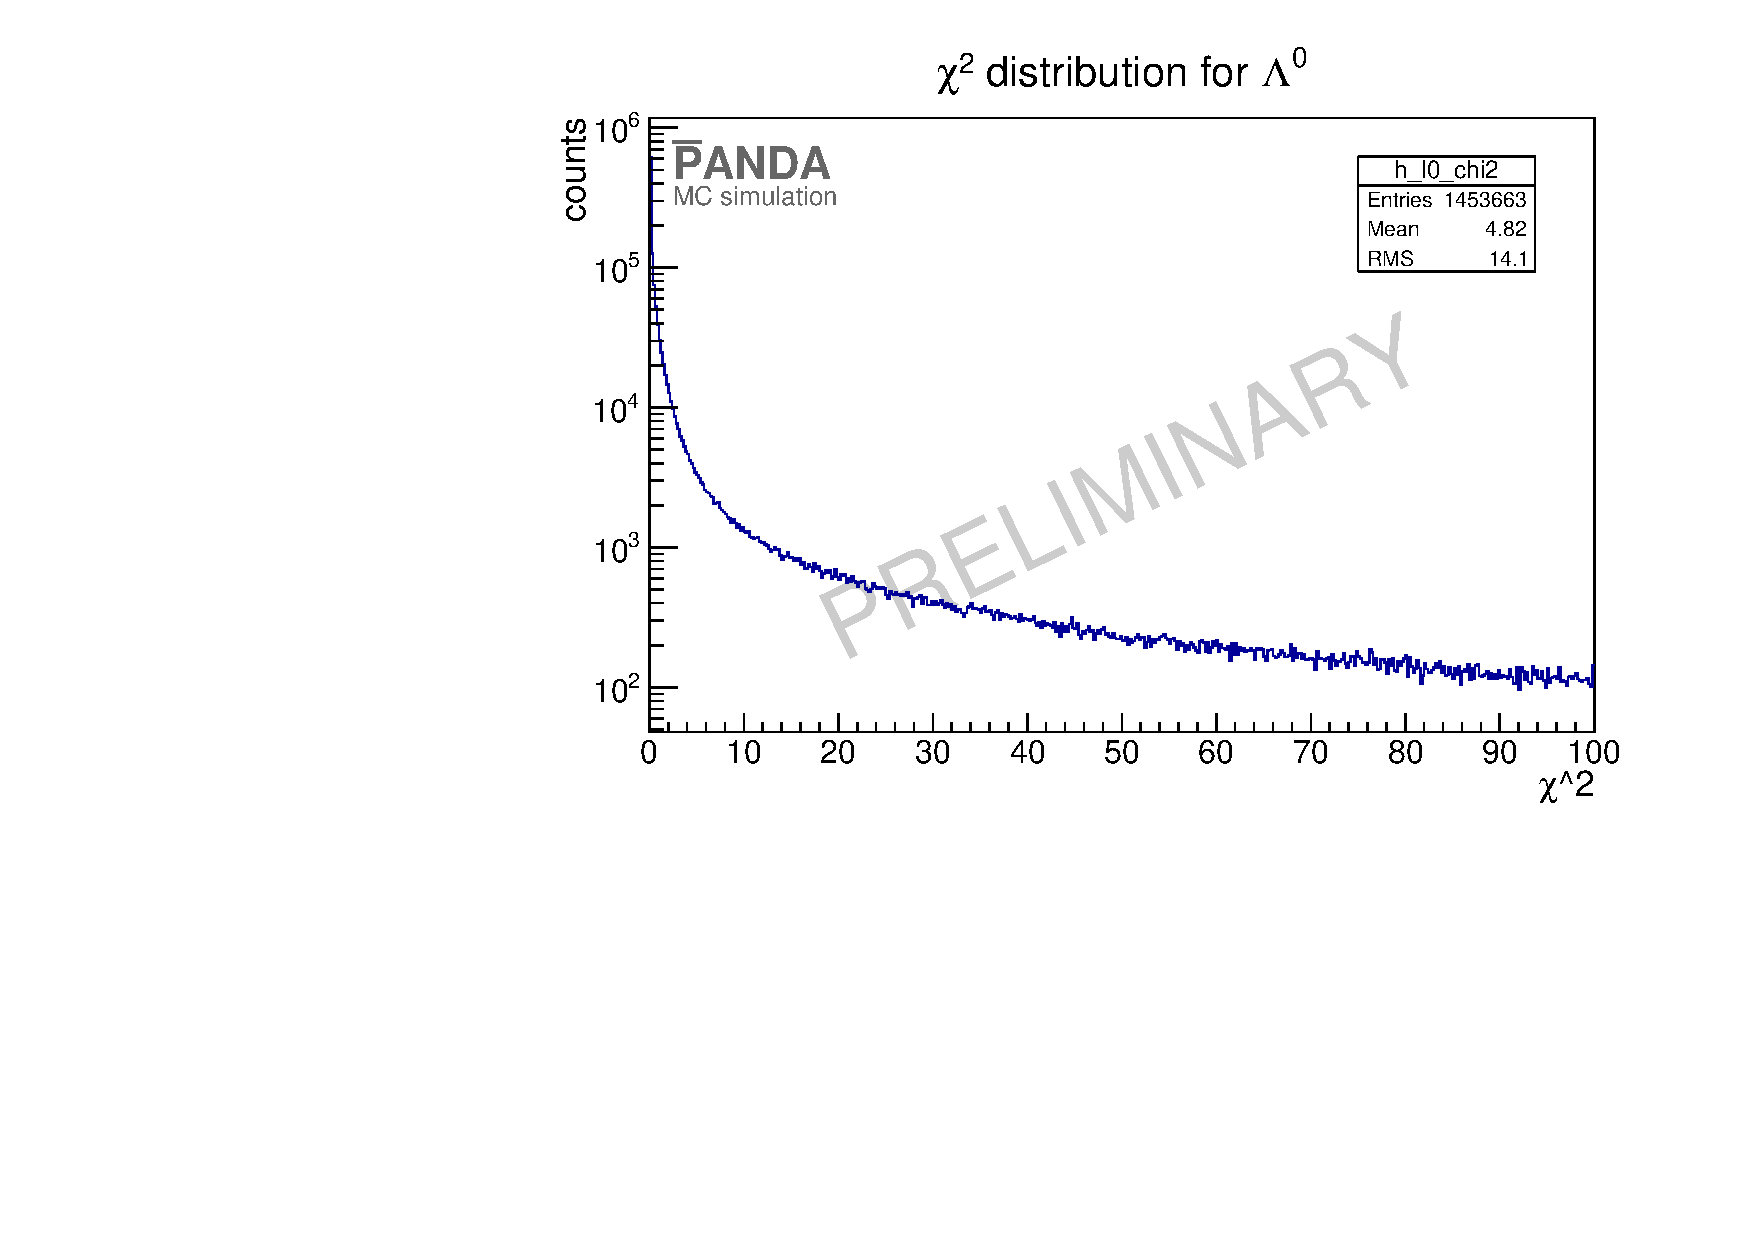
\includegraphics[width=0.50\textwidth]{./plots/lambda0/lambda0_chisqrt.pdf}
				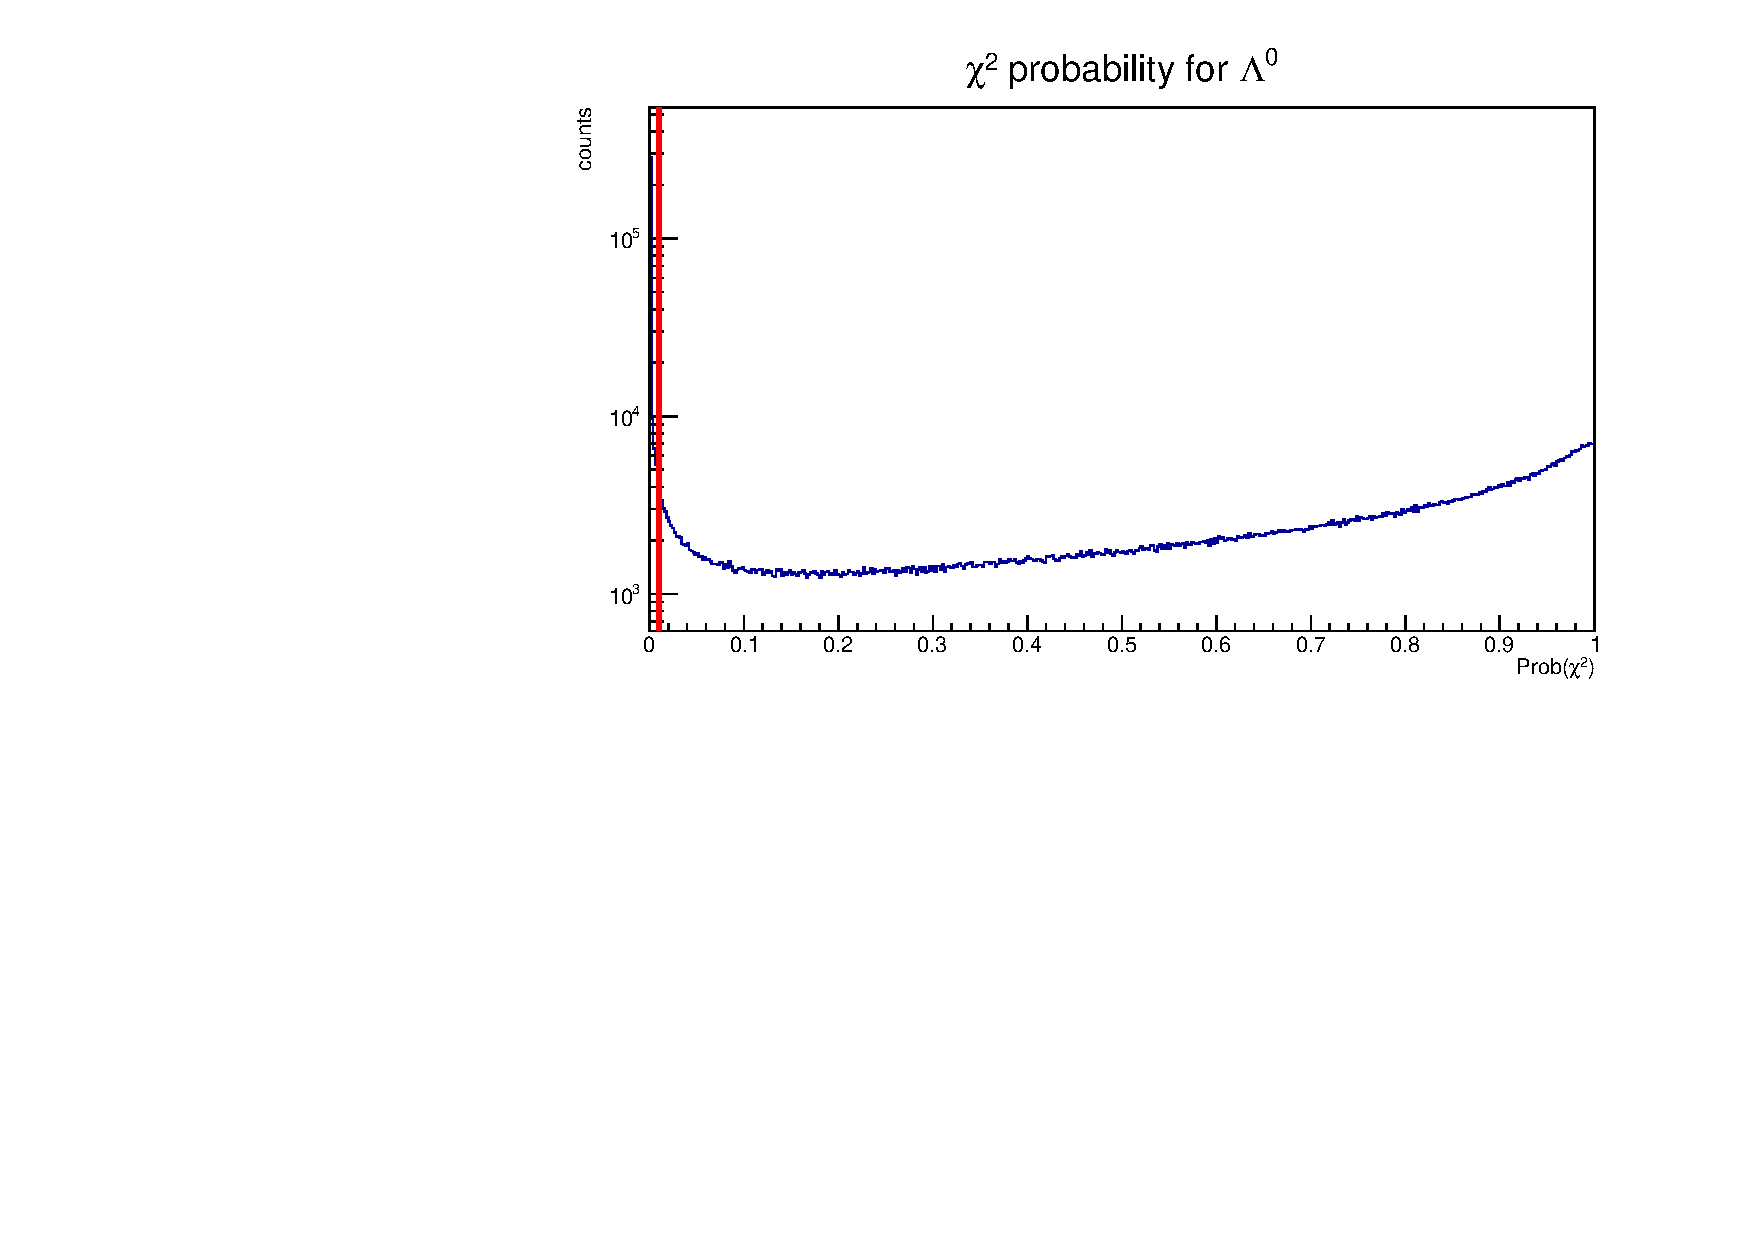
\includegraphics [width=0.50\textwidth]{./plots/lambda0/lambda0_prob.pdf}
			\caption{upper: \chisq distribution; lower: \chisq probability distribution}
			\label{fig:lambda_chi2}
		\end{figure}
		
		In the \chisq-probability distribution one can see a increasing number of events for probabilites going to one.
		These feature is not coming from vertex fitting.
		There is still a problem with covariance matrices which causes the effect.
		\vspace{11pt}\\
		The fit information coming from the vertex fit are used to perform a mass contraint fit with the kinematic fitter PndKinFitter.
		After using both fitter the selection criterion is set. 
		One select only those particles which have a probabiltiy greater than $1\%$ in both fitter.
		A scheme which shows how the events are selected can be found in figure \ref{fig:lambda_scheme}. 
		
		\begin{figure}
			\centering
				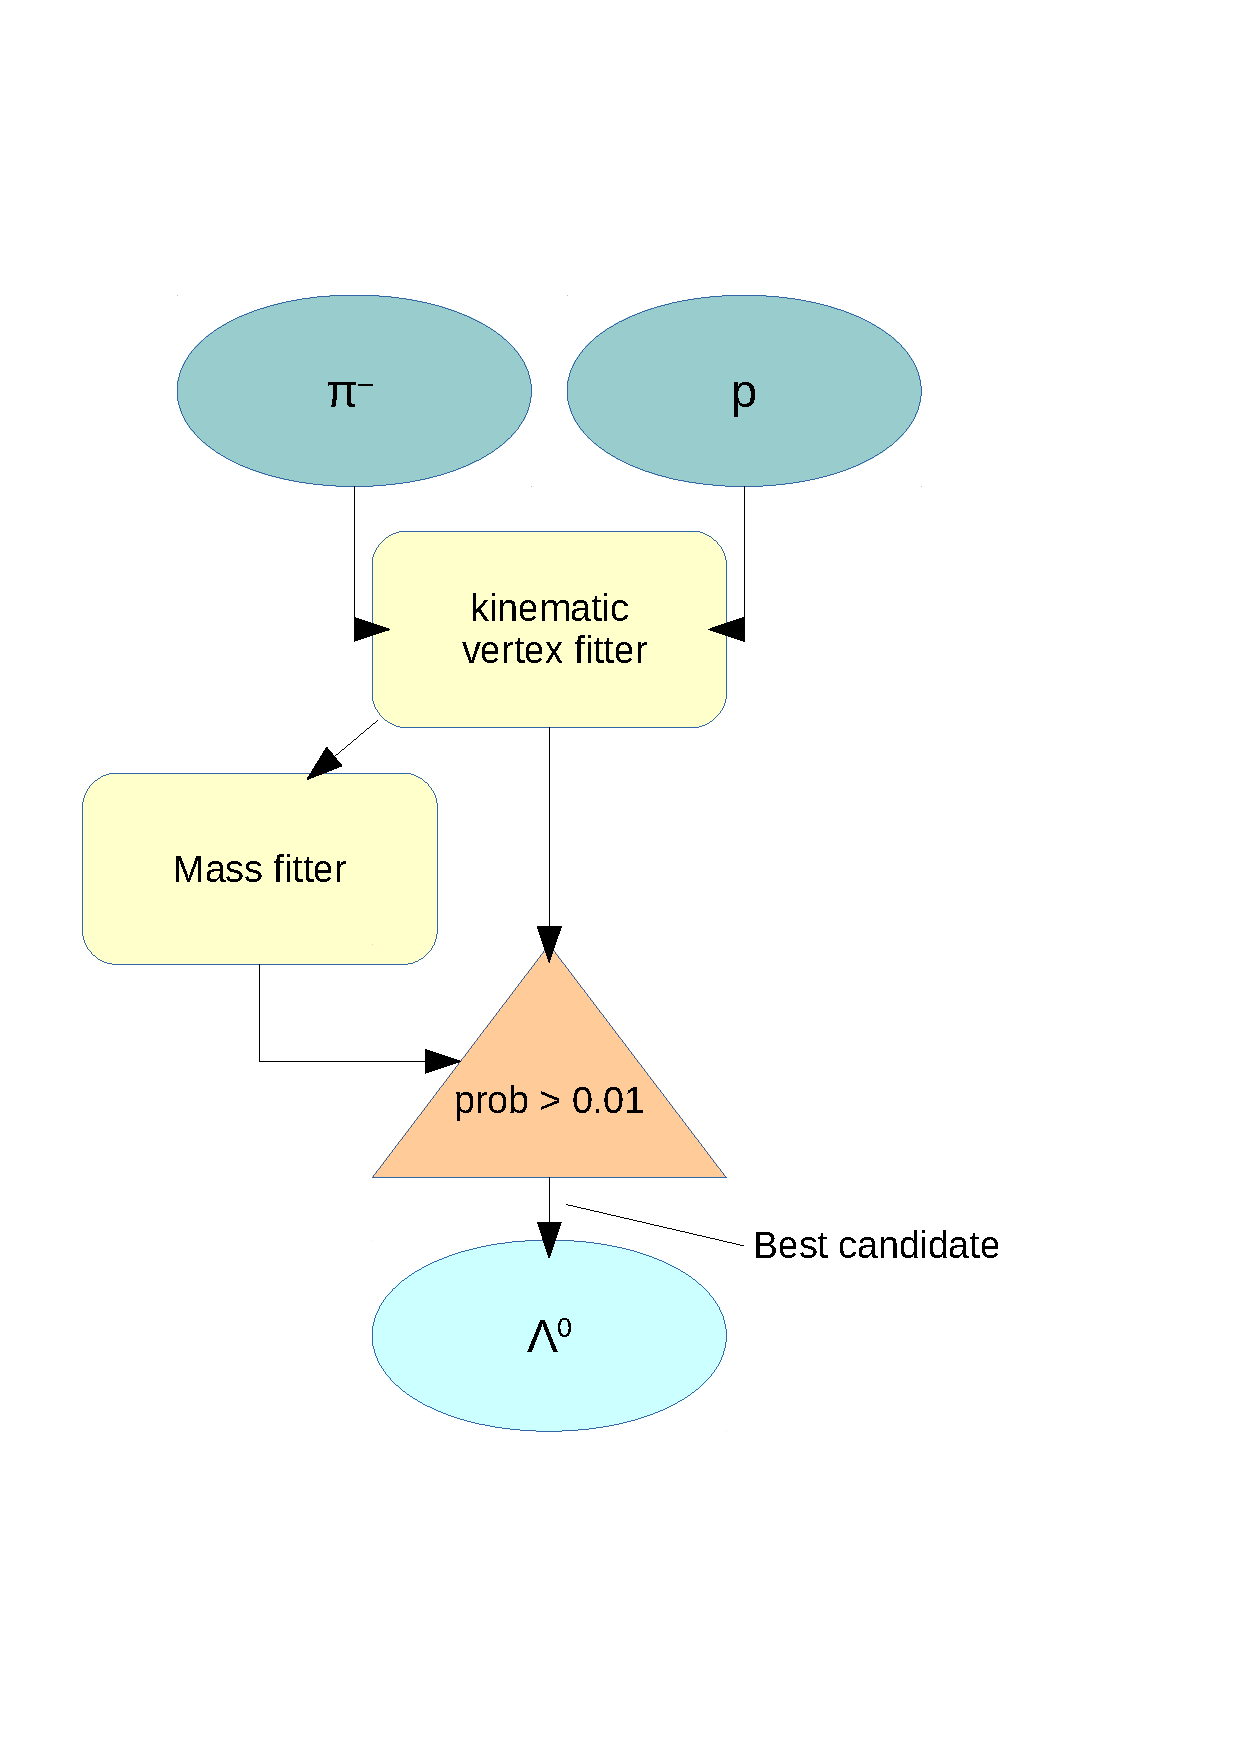
\includegraphics[width=0.50\textwidth]{./plots/combineLambda0.pdf}
			\caption{Scheme for \lam reconstruction}
			\label{fig:lambda_scheme}
		\end{figure}
		
		If there is more than one candidate left after the cuts the best fitted candidate is chosen.
		
		
	\subsection*{Results}
		This subsection presents the results for the \lam and \alam selection with the selection criteria introduced above.
		The mass distributions for different cuts are shown in figure \ref{fig:lambda0_massdiffcuts} and figure \ref{fig:antilambda0_massdiffcuts}.
	
		\begin{figure}
			\centering
				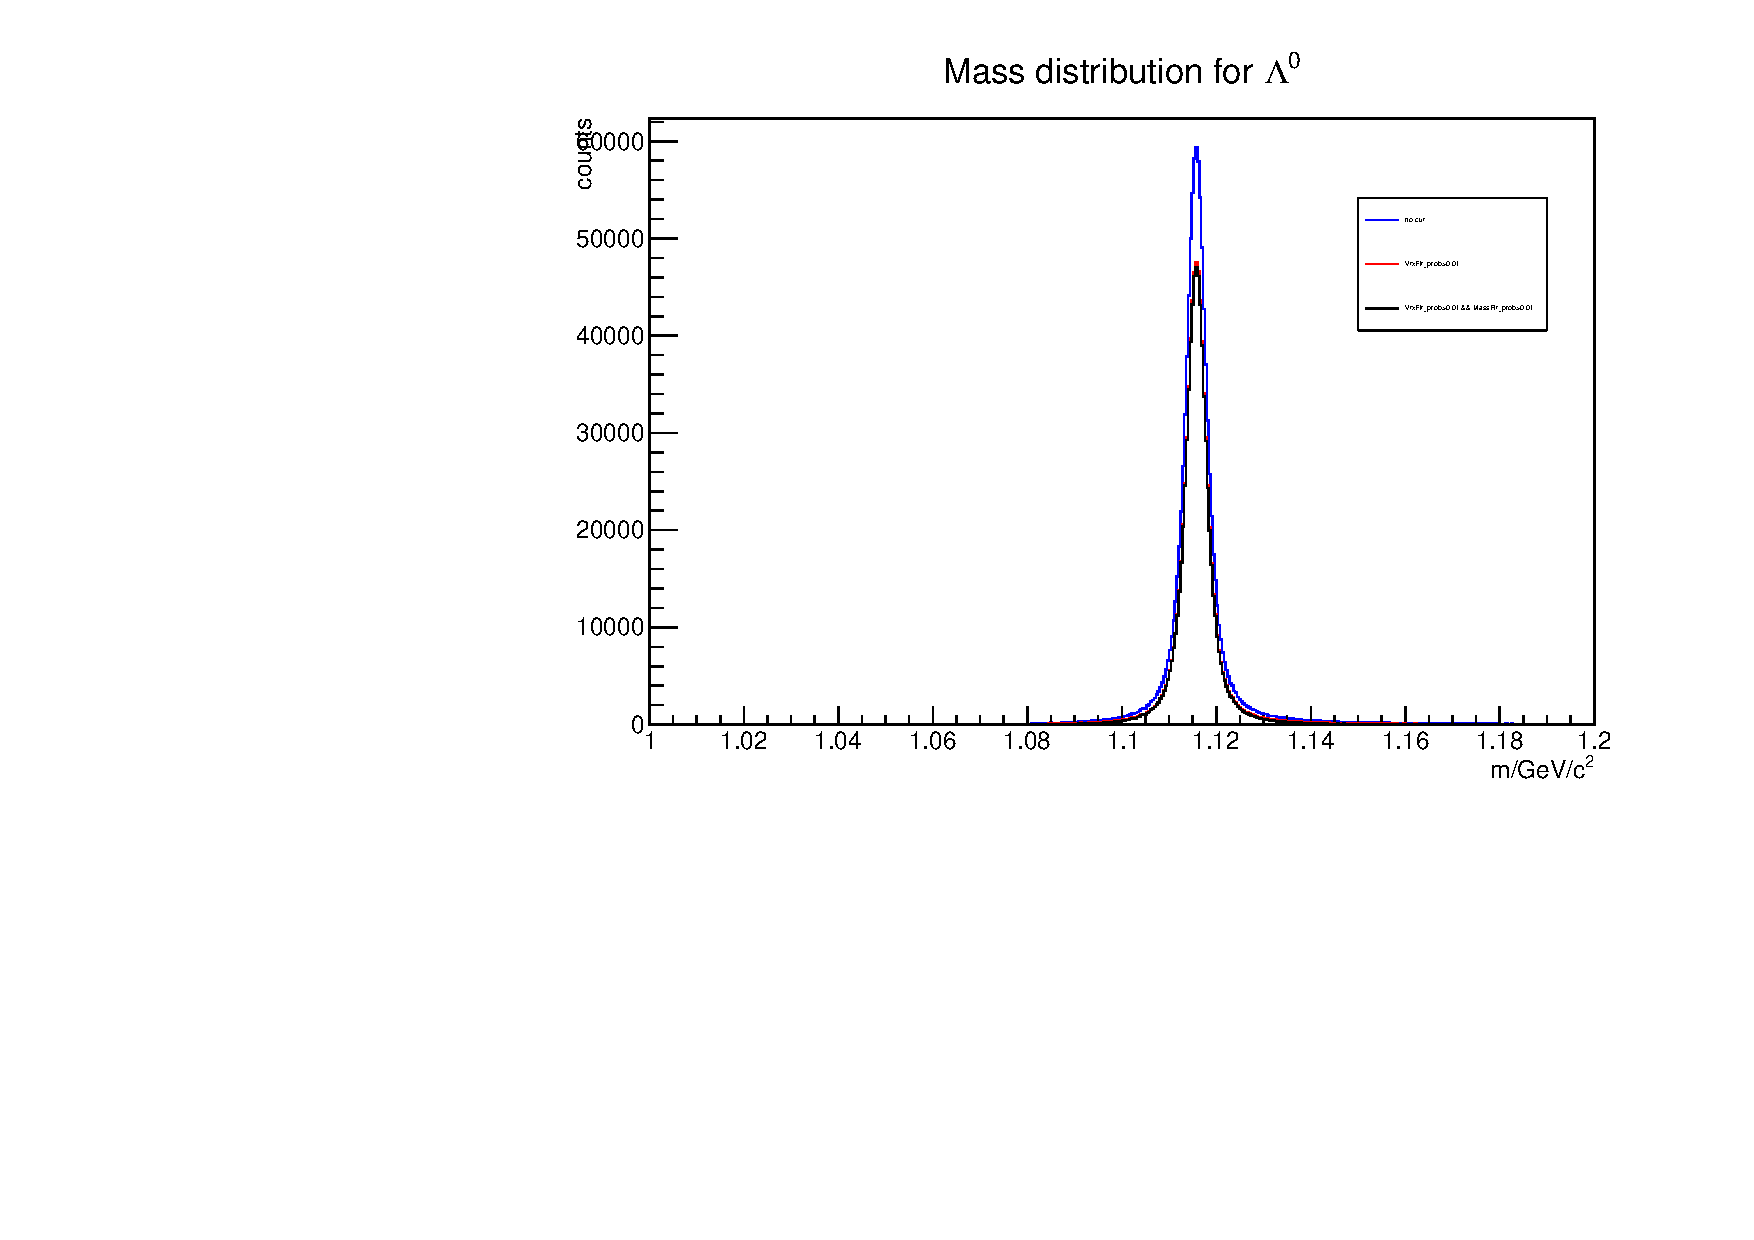
\includegraphics[width=1.1\textwidth]{./plots/lambda0/lambda0_m_diffcuts.pdf}
			\caption{Mass distribution of \lam for different cuts}
			\label{fig:lambda0_massdiffcuts}
			
				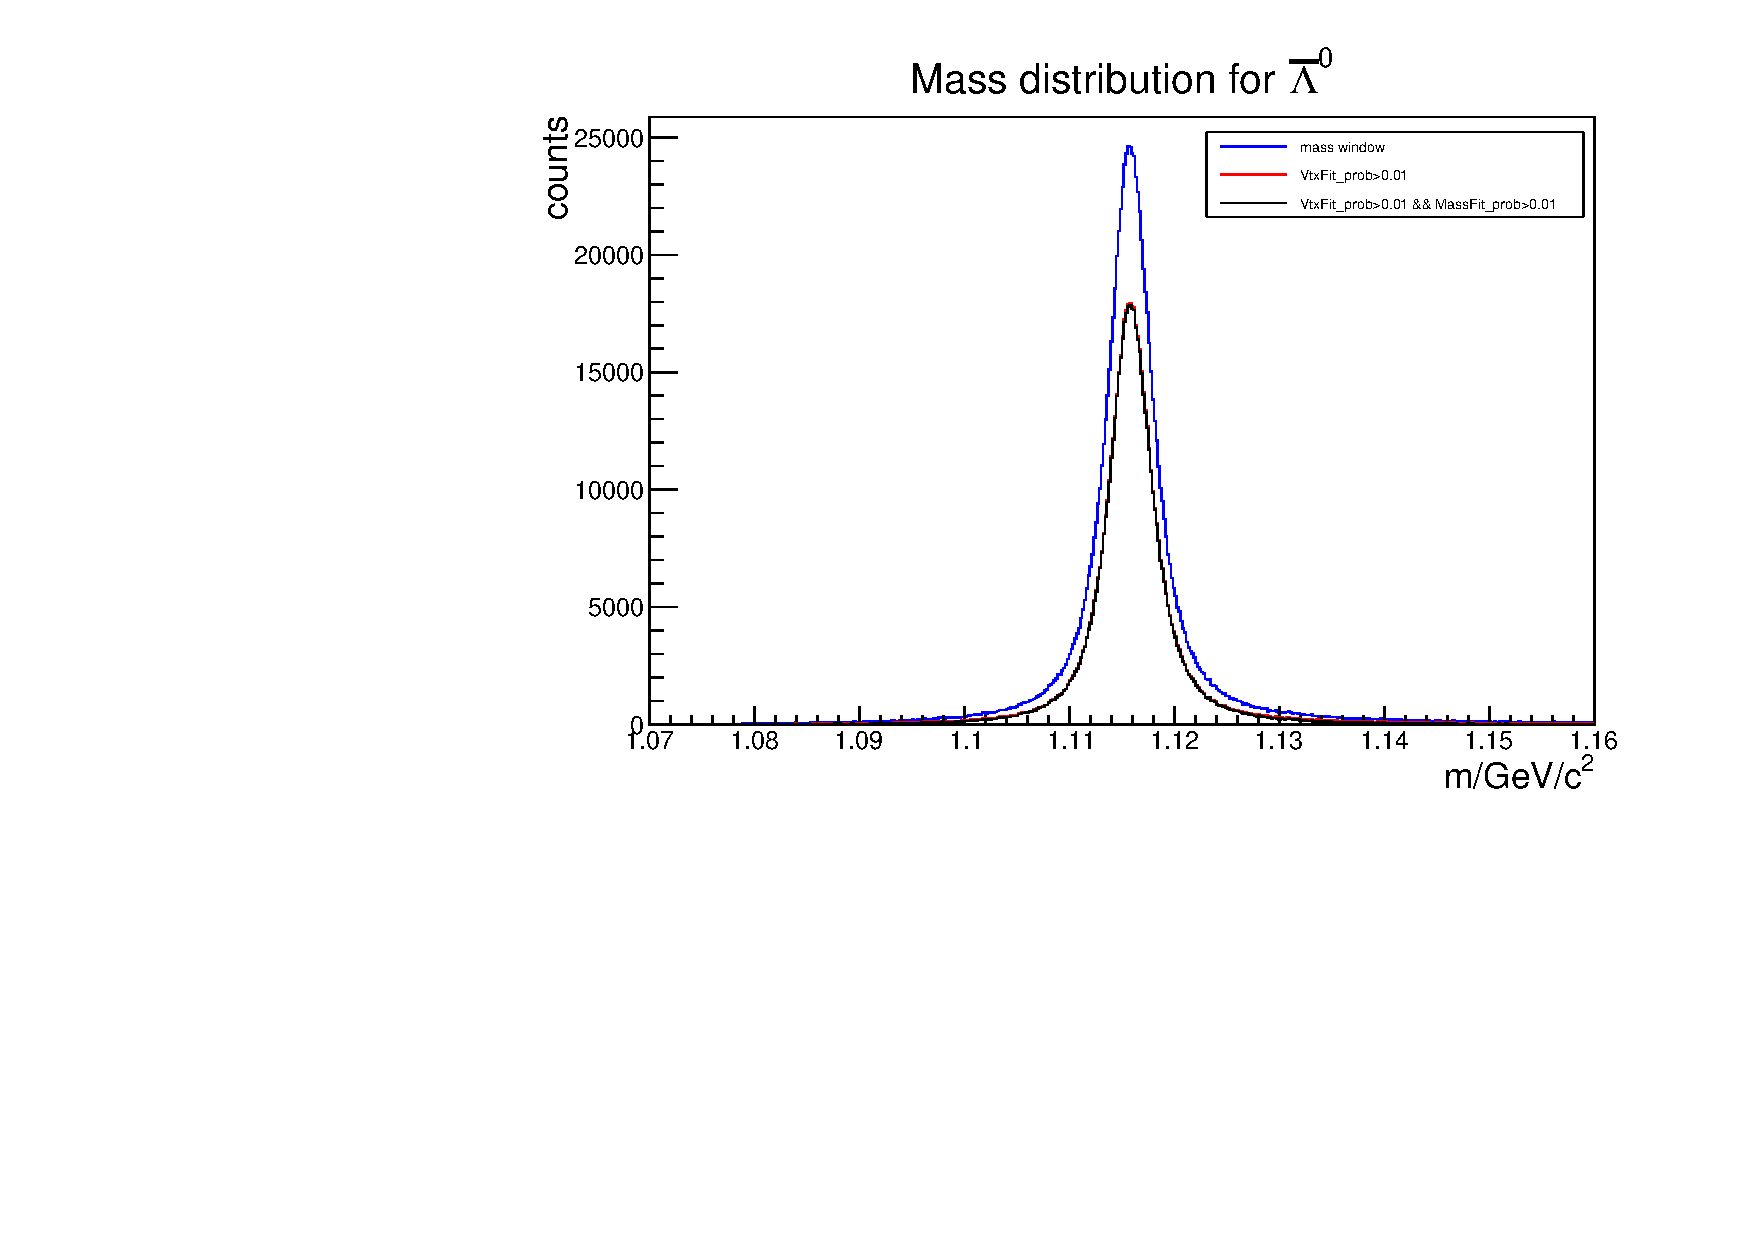
\includegraphics[width=1.1\textwidth]{./plots/antilambda0/antiLambda0_m_diffcuts.pdf}
			\caption{Mass distribution of \alam for different cuts}
			\label{fig:antilambda0_massdiffcuts}
		\end{figure}
		
		The reconstructed mass can be derived by performing a doulbe gaussian fit on the cutted mass.
		The mass distribution and the double gausssian fit are exemplarily shown for \lam in figure \ref{fig:lambda0_massfit}
		
		\begin{figure}
			\centering
				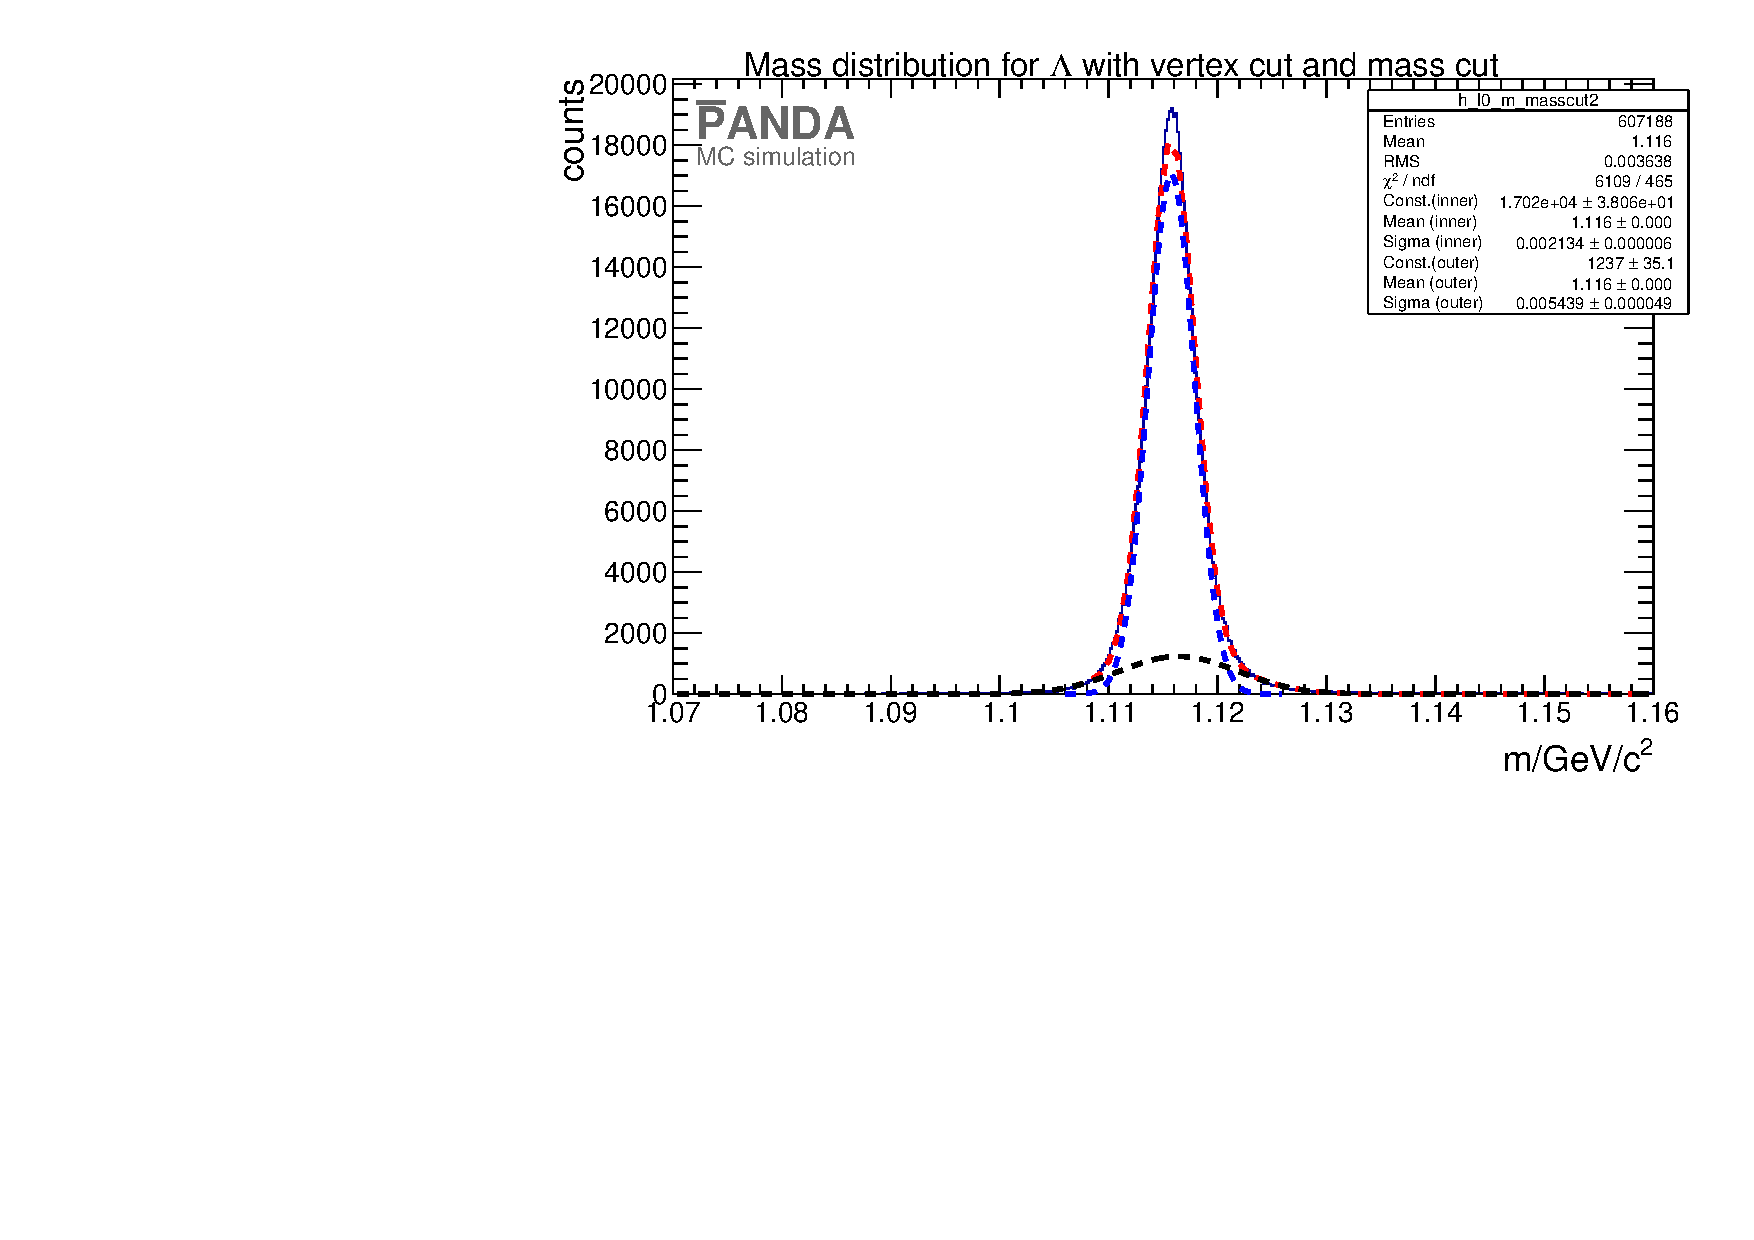
\includegraphics[width=0.8\textwidth]{./plots/lambda0/lambda0_m_masscut2.pdf}
			\caption{Mass distribution -- blue line -- for \lam fitted with a double gaussian fit shown as red dashed line.}
			\label{fig:lambda0_massfit}
		\end{figure}
		
		The mean value of the inner gaussian fit is the reconstructed mass.
		The result for \lam is $\mt{m}_{\Lambda^0} = \left(1.116 \pm 3.5\cdot 10^{-5}\right)$ \massunit and for \alam: $\mt{m}_{\bar{\Lambda}^0} = \left(1.116 \pm 1\cdot 10^{-5}\right)$\massunit. 
		The small fit errors could be a result from the wrong covariance matrices. 
		But this has to be checked. 
		Figure \ref{fig:lambda0_pt_vs_pz} shows the transverse momentum versus the longitudinal momentum.
				
		\begin{figure}
			
			\subfigure[]{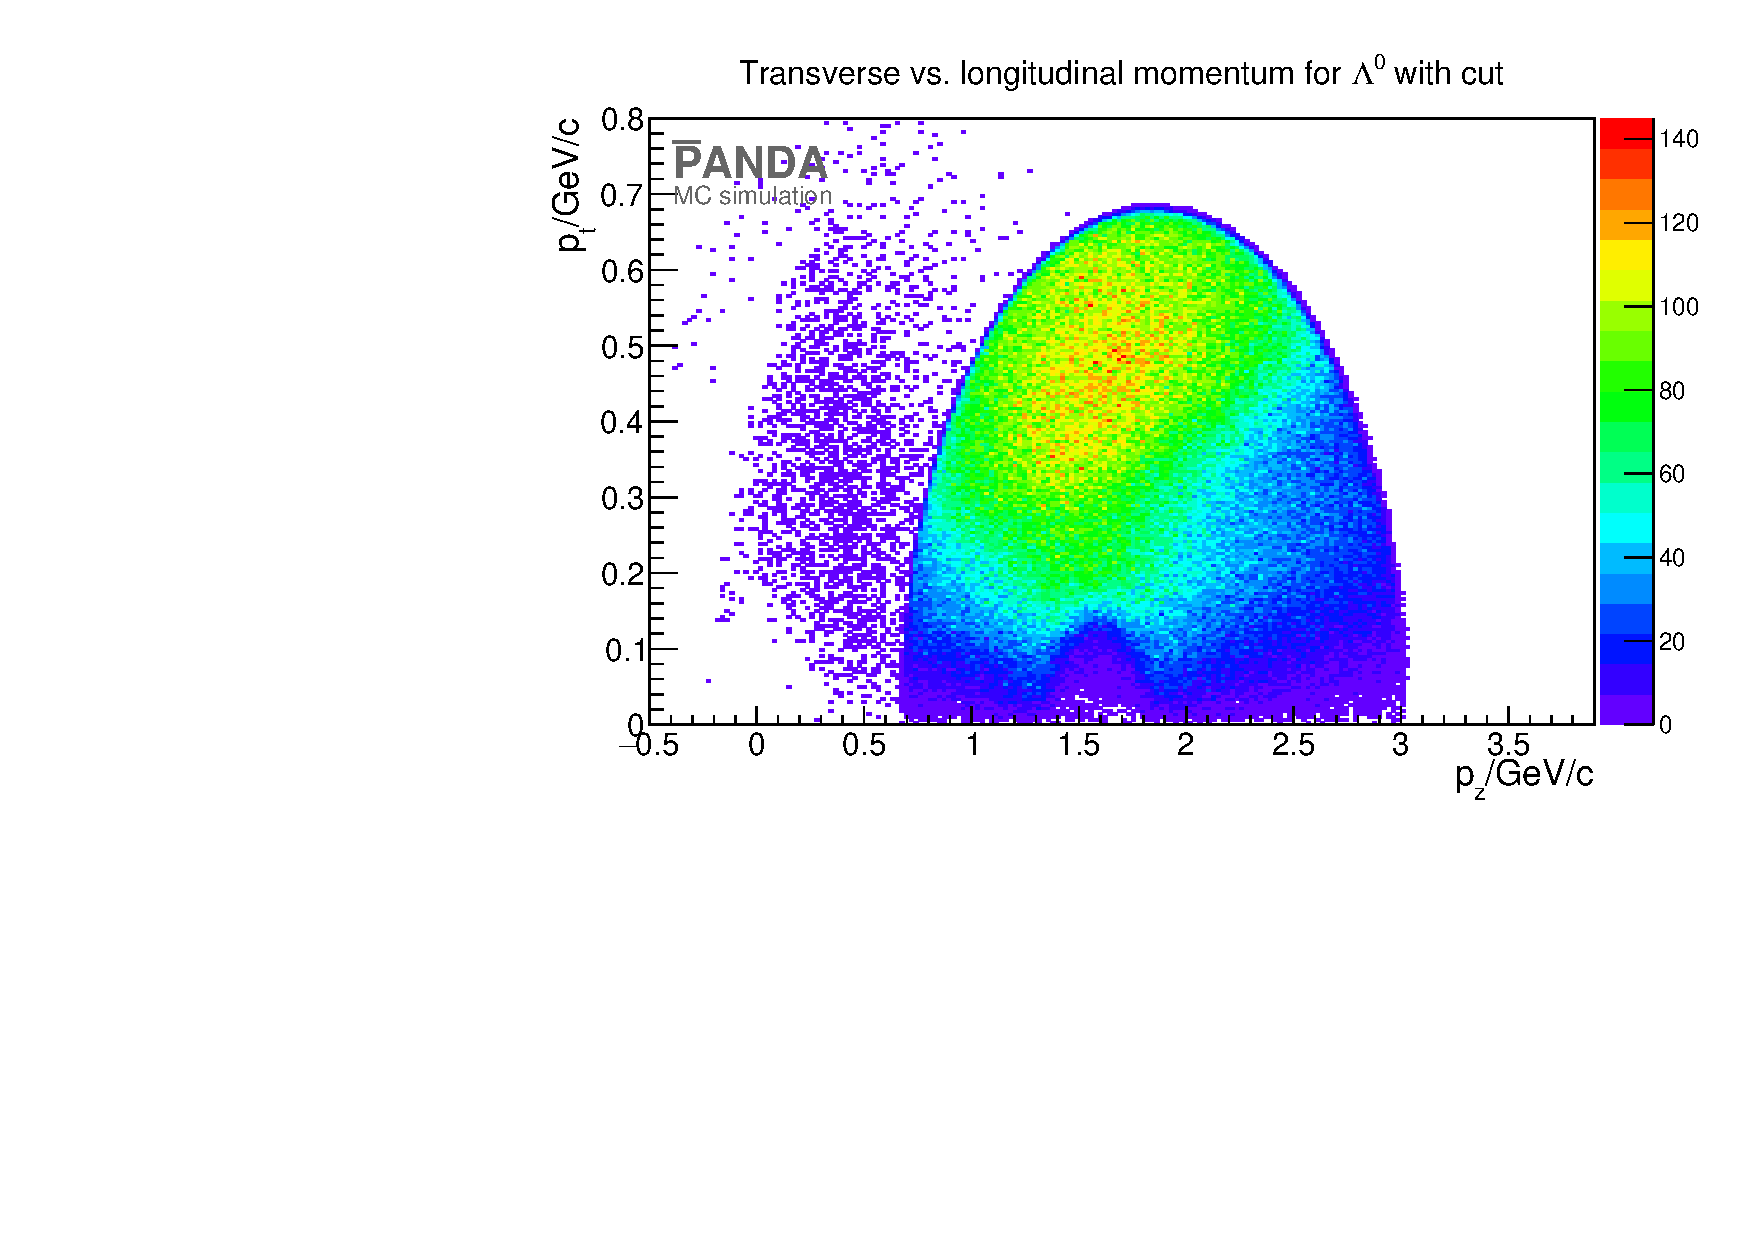
\includegraphics[width=0.49\textwidth]{./plots/lambda0/lambda0_pt_vs_pz_cut.pdf}}
			\subfigure[]{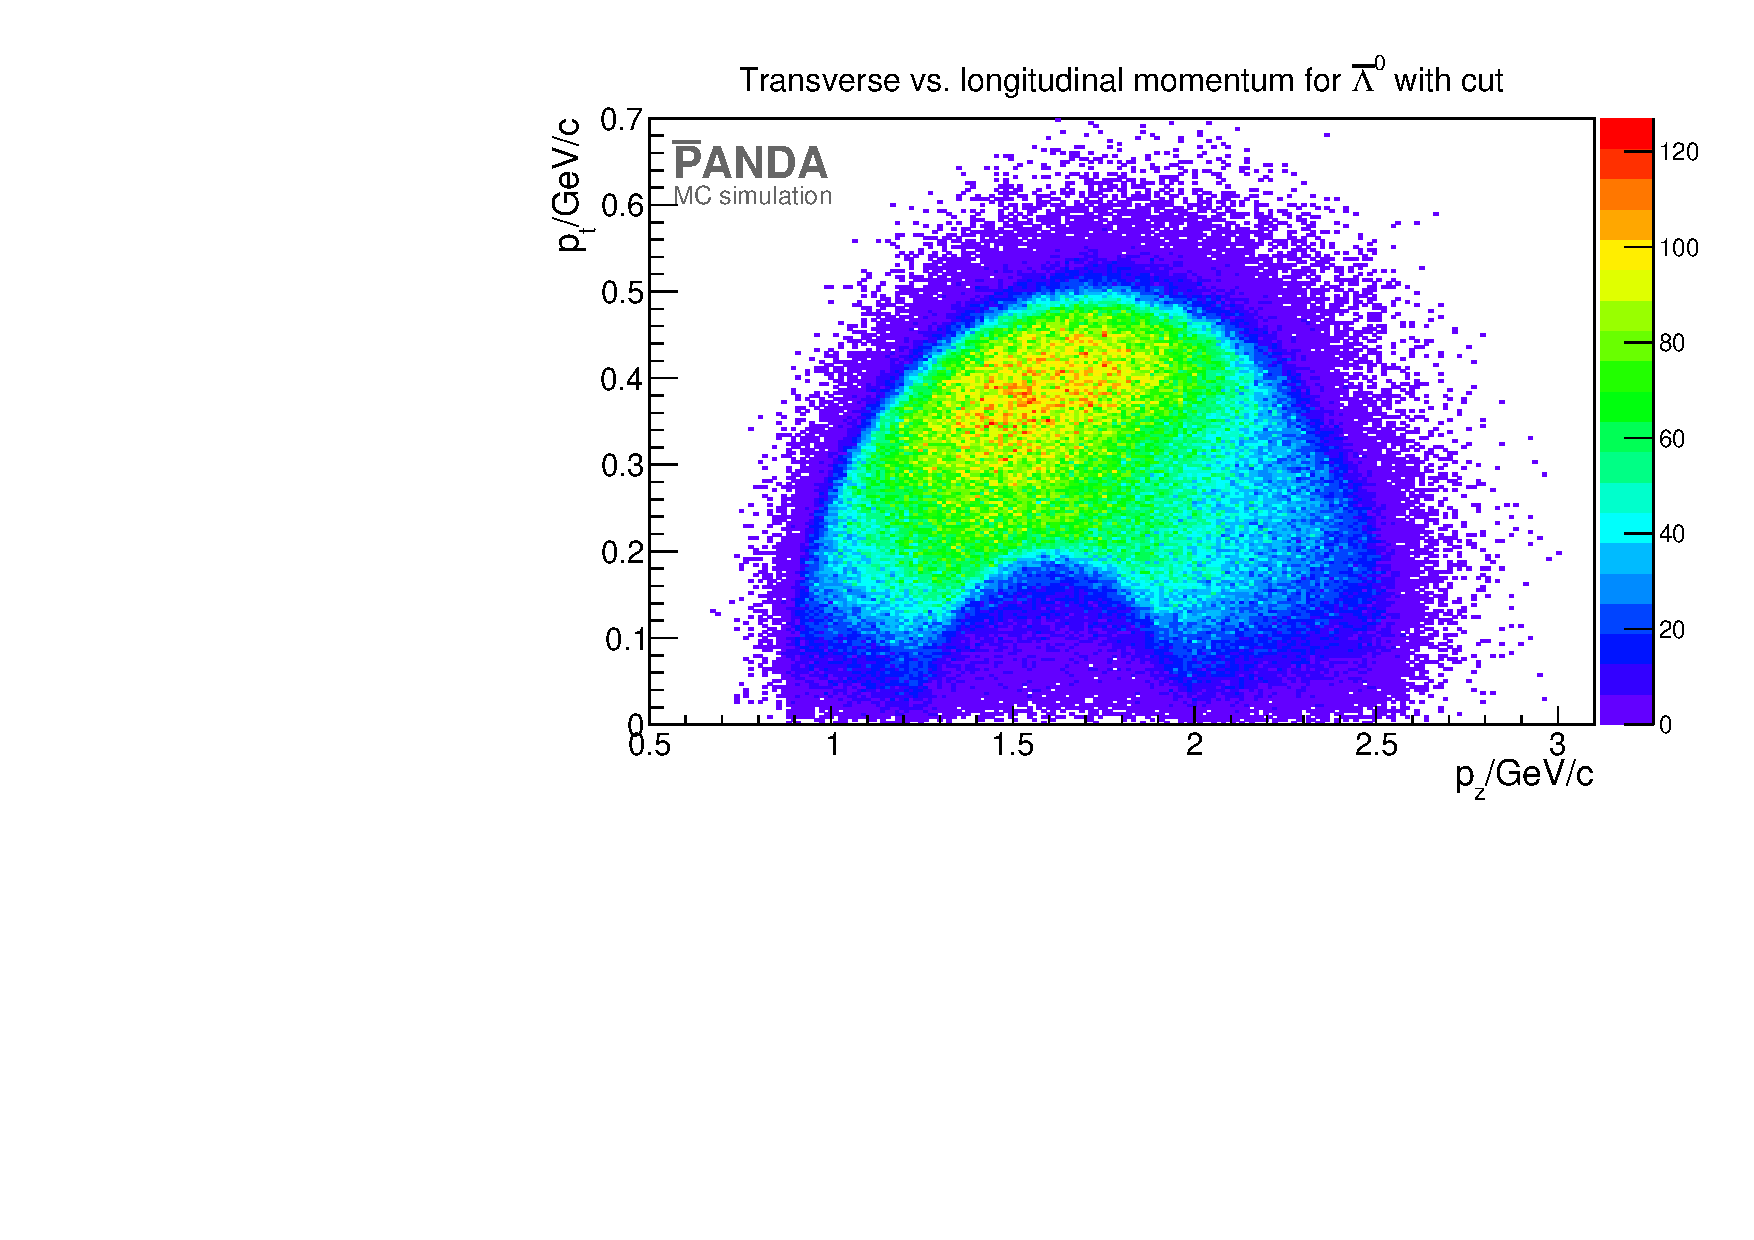
\includegraphics[width=0.49\textwidth]{./plots/antilambda0/antiLambda0_pt_vs_pz_cut.pdf}}
			\caption{The plots shows the transverse against the longuitudinal momentum for \lam}
			\label{fig:lambda0_pt_vs_pz}
		
		\end{figure}
		After all cuts the reconstruction efficiency for \lam is $50.33\%$ and for \alam $41.46\%$.
		The difference of the reconstruction efficiency of \lam and \alam is caused by the difference between the decay length of their mother particles.
		\lam is emitted by the \excitedcascade which has a very short decay length while the decay length of \cascade and \anticascade is c$\tau = 4.91 \unit{cm}$ \cite{PDG}.
		In addition the decay length of \lam and \alam is $\textnormal{c}\tau = 7.98 \unit{cm}$.
		If one sum this number up the final state particles of \alam are produced more downstream than the final state particles of \lam.
		This can be also seen in figure \ref{fig:lambda0_antilambda0_decay_vtx}.
		The finale state particles coming from \alam are produced at the edge of the MVD detector so that the reconsturction efficiency get worse.
		
		\begin{figure}
		
			\centering
			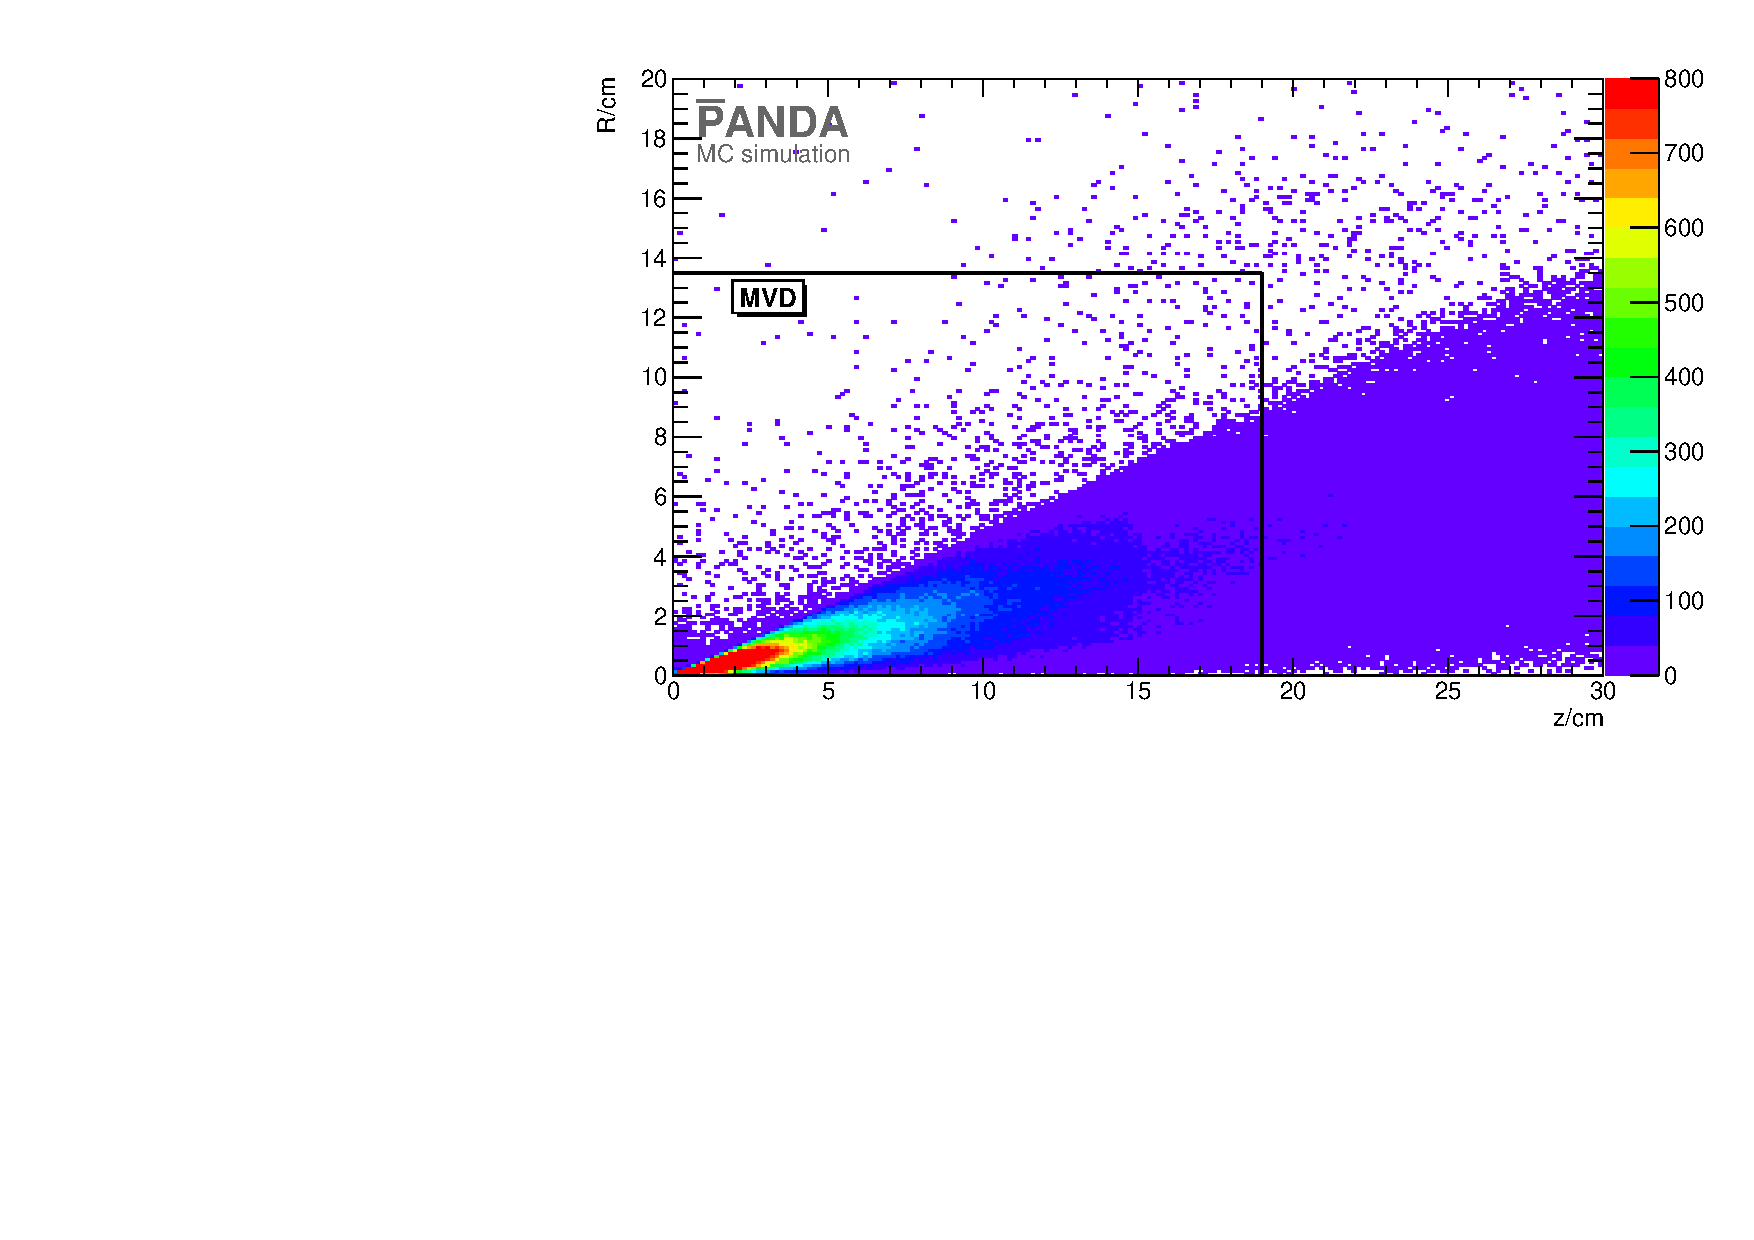
\includegraphics[width=1.\textwidth]{./plots/lambda0/lambda0_decay_vtx.pdf}
			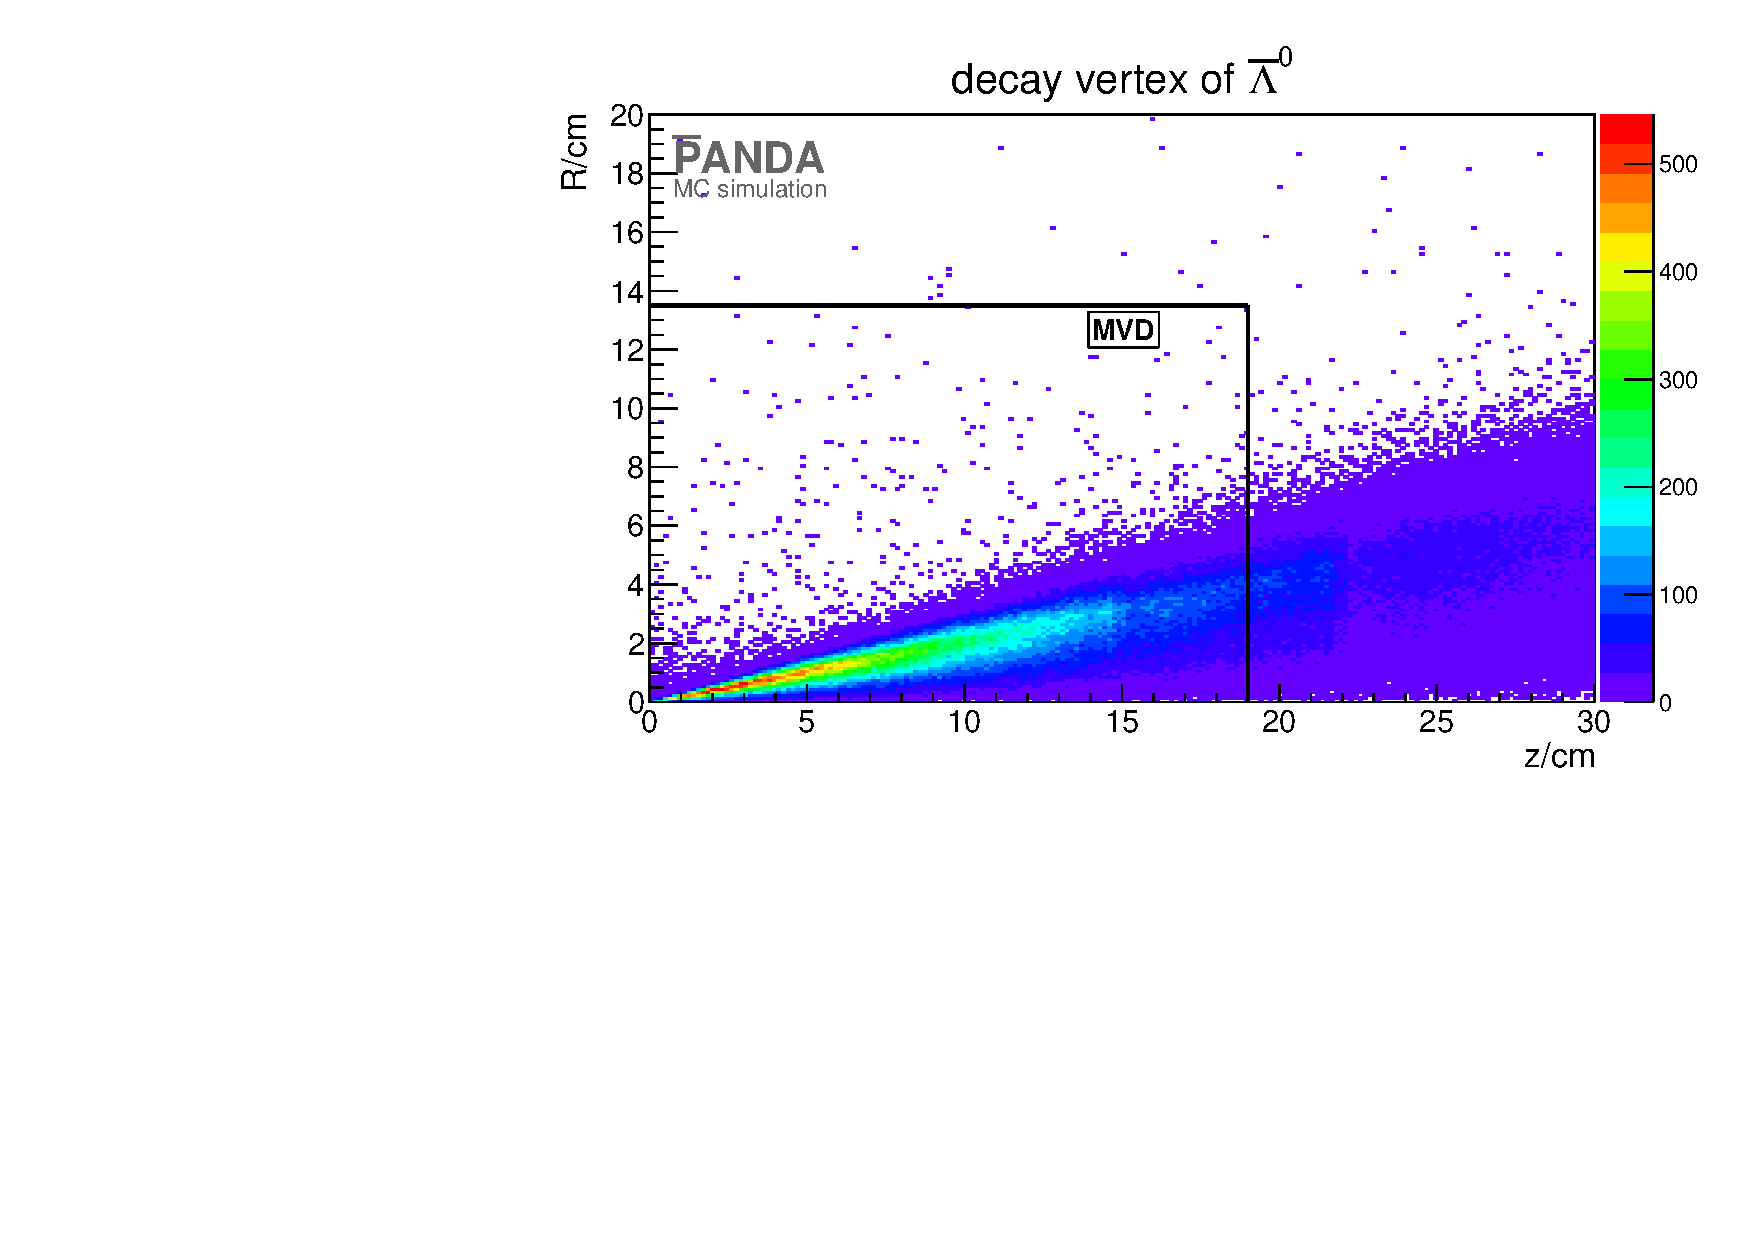
\includegraphics[width=1.\textwidth]{./plots/antilambda0/antiLambda0_decay_vtx.pdf}
			\caption{Upper plot shows the decay vertex of \lam; lower plot shows decay vertex of \alam}
			\label{fig:lambda0_antilambda0_decay_vtx}
		
		\end{figure}
		
		
		
		
	
\section{Reconstruction of $\boldmath{\Xi}$ and $\boldmath{\bar{\Xi}}$}
	\subsection*{Selection}
		The reconstruction of \cascade and \anticascade fellow a similar scheme like for \lam and \alam.
		For \anticascade are \alam and \piplusone recombined and for \cascade in the c.c. channel \lam and \piminusone.
		Now it is distinguished between the to \piplus (\piminus) particle and use only those particles which have not already been combined.
		After combining the daughter particles it is performed a mass window cut with width of $0.3$\massunit 
		arraound the \cascade mass $m_{\Xi} = 1.32171$ \massunit \cite{PDG}.
		 
		The fitting scheme is the same as for \lam and \alam and is shown in figure \ref{fig:anticascade_scheme} 
		After the mass window cut the daughter particles are fitted to a common vertex with the PndKinVtxFitter.
		And again these information is used to perform the mass constraint fitter. 
		
		\begin{figure}
			\centering
				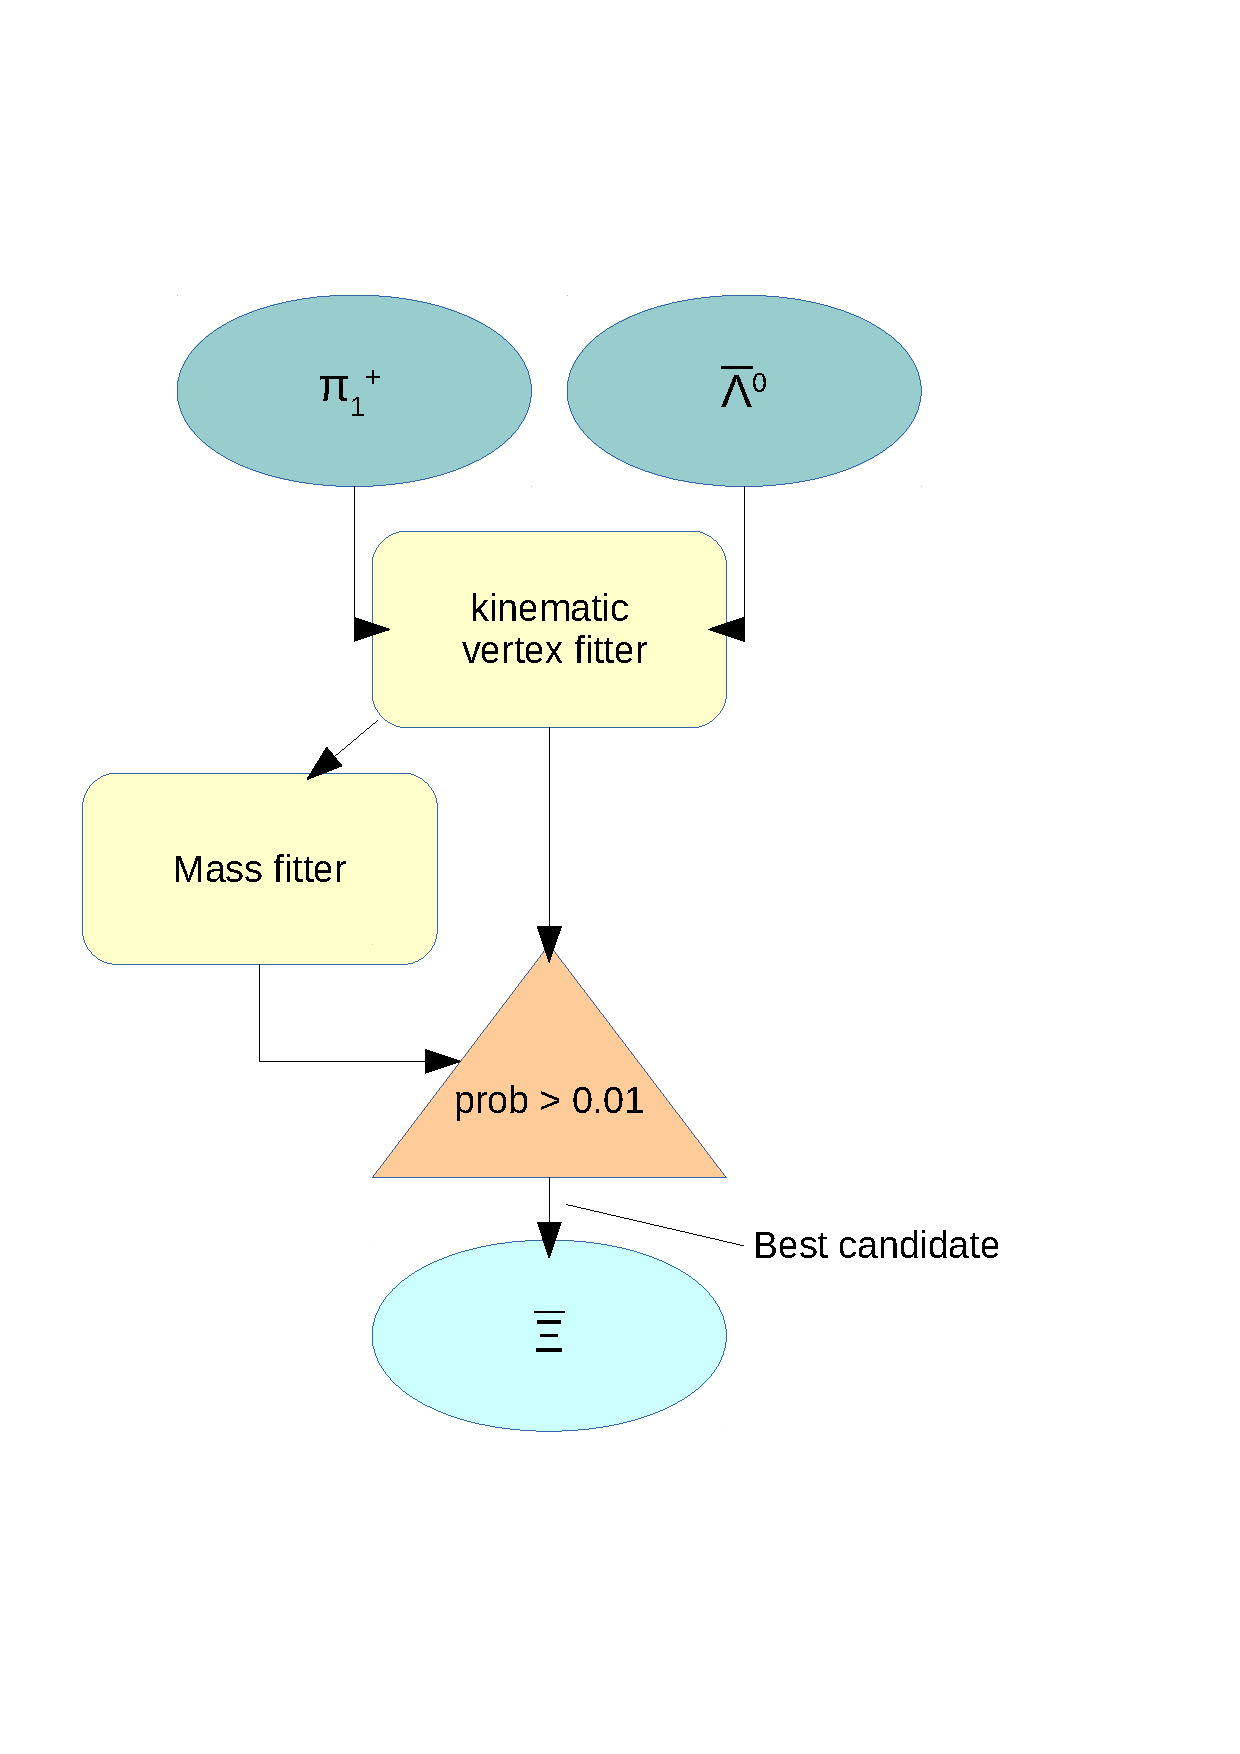
\includegraphics[width=0.50\textwidth]{./plots/combineAntiCascade.pdf}
			\caption{Scheme for \anticascade reconstruction}
			\label{fig:anticascade_scheme}
		\end{figure}
		
		Only those particles are selected which have a \chisq probability of more than $1\,\%$ in both fitter. 
		Figure \ref{fig:XiPlus_prob} shows exemplarily the cut on the vertex fit probability.
		
		\begin{figure}
			\centering
				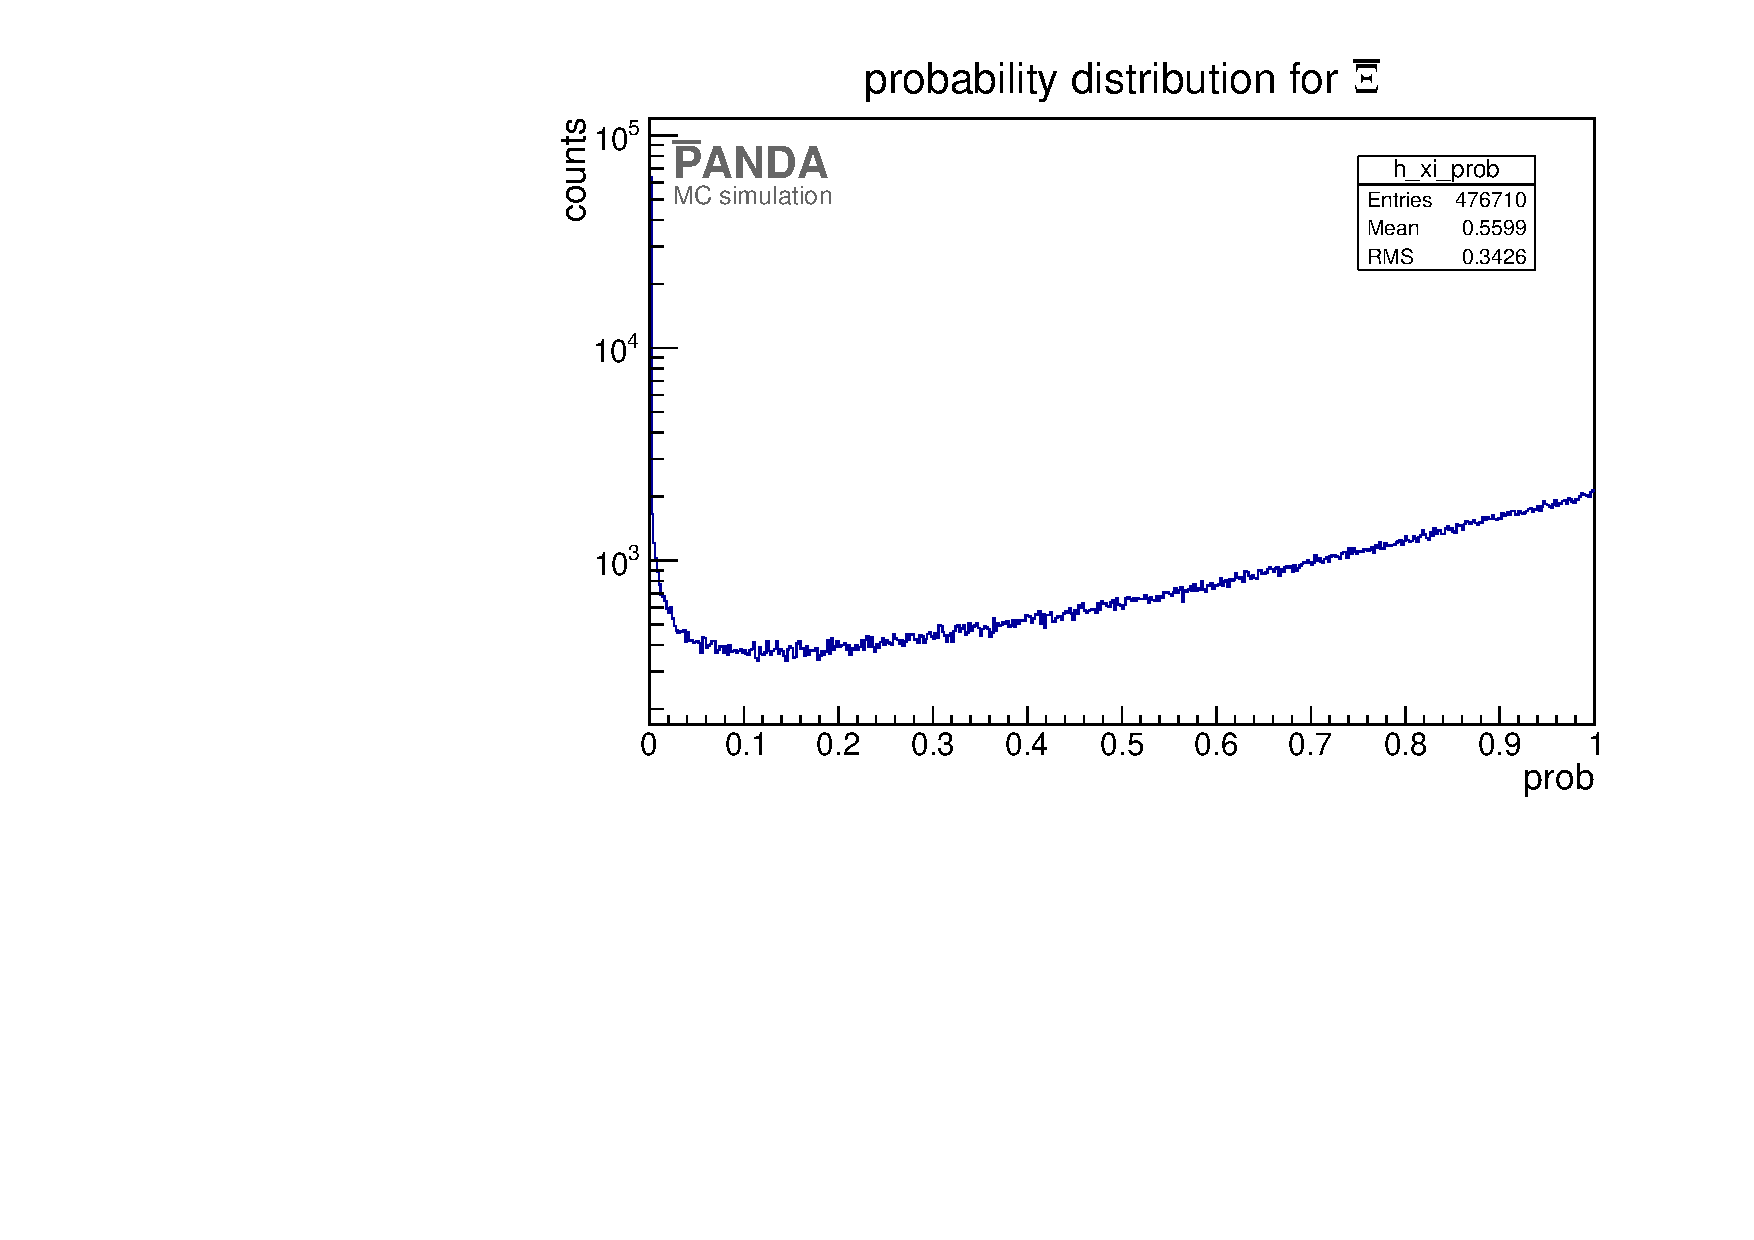
\includegraphics[width=0.50\textwidth]{./plots/Xi/XiPlus_prob.pdf}
			\caption{\chisq probalility for \anticascade reconstruction}
			\label{fig:XiPlus_prob}
		\end{figure}
			
		If there is more than one candidate left after all cuts the best candidate is chosen.
		
		
	\subsection*{Results}
		The vertex resolution after all cuts is shown in table \ref{tab:XiPlus_vtxres}. 
		
		\begin{table}
			\centering
			\caption{Vertex resolution for \anticascade and \cascade (c.c. channel)}
			\label{tab:XiPlus_vtxres}
			\begin{tabular}{ccc}
				\hline
				position & \anticascade & \cascade(from c.c.) \\\hline
				\hline
				x/cm & $0.052$ & $0.056$\\
				y/cm & $0.052$ & $0.052$\\
				z/cm & $0.192$ & $0.2$\\
				\hline
				    
			\end{tabular}
		\end{table}
		
		It is determined by calculating the full width at half maximum (FWHM) of the distribution.
		The advantage of using this method to calculated the vertex resolution is that the FWHM is independent of distribution shape.
		Figure \ref{fig:xi_vtxres_x} and Figure \ref{fig:xi_vtxres_yz} show the vertex resolution. 
		
		\begin{figure}
			\centering
			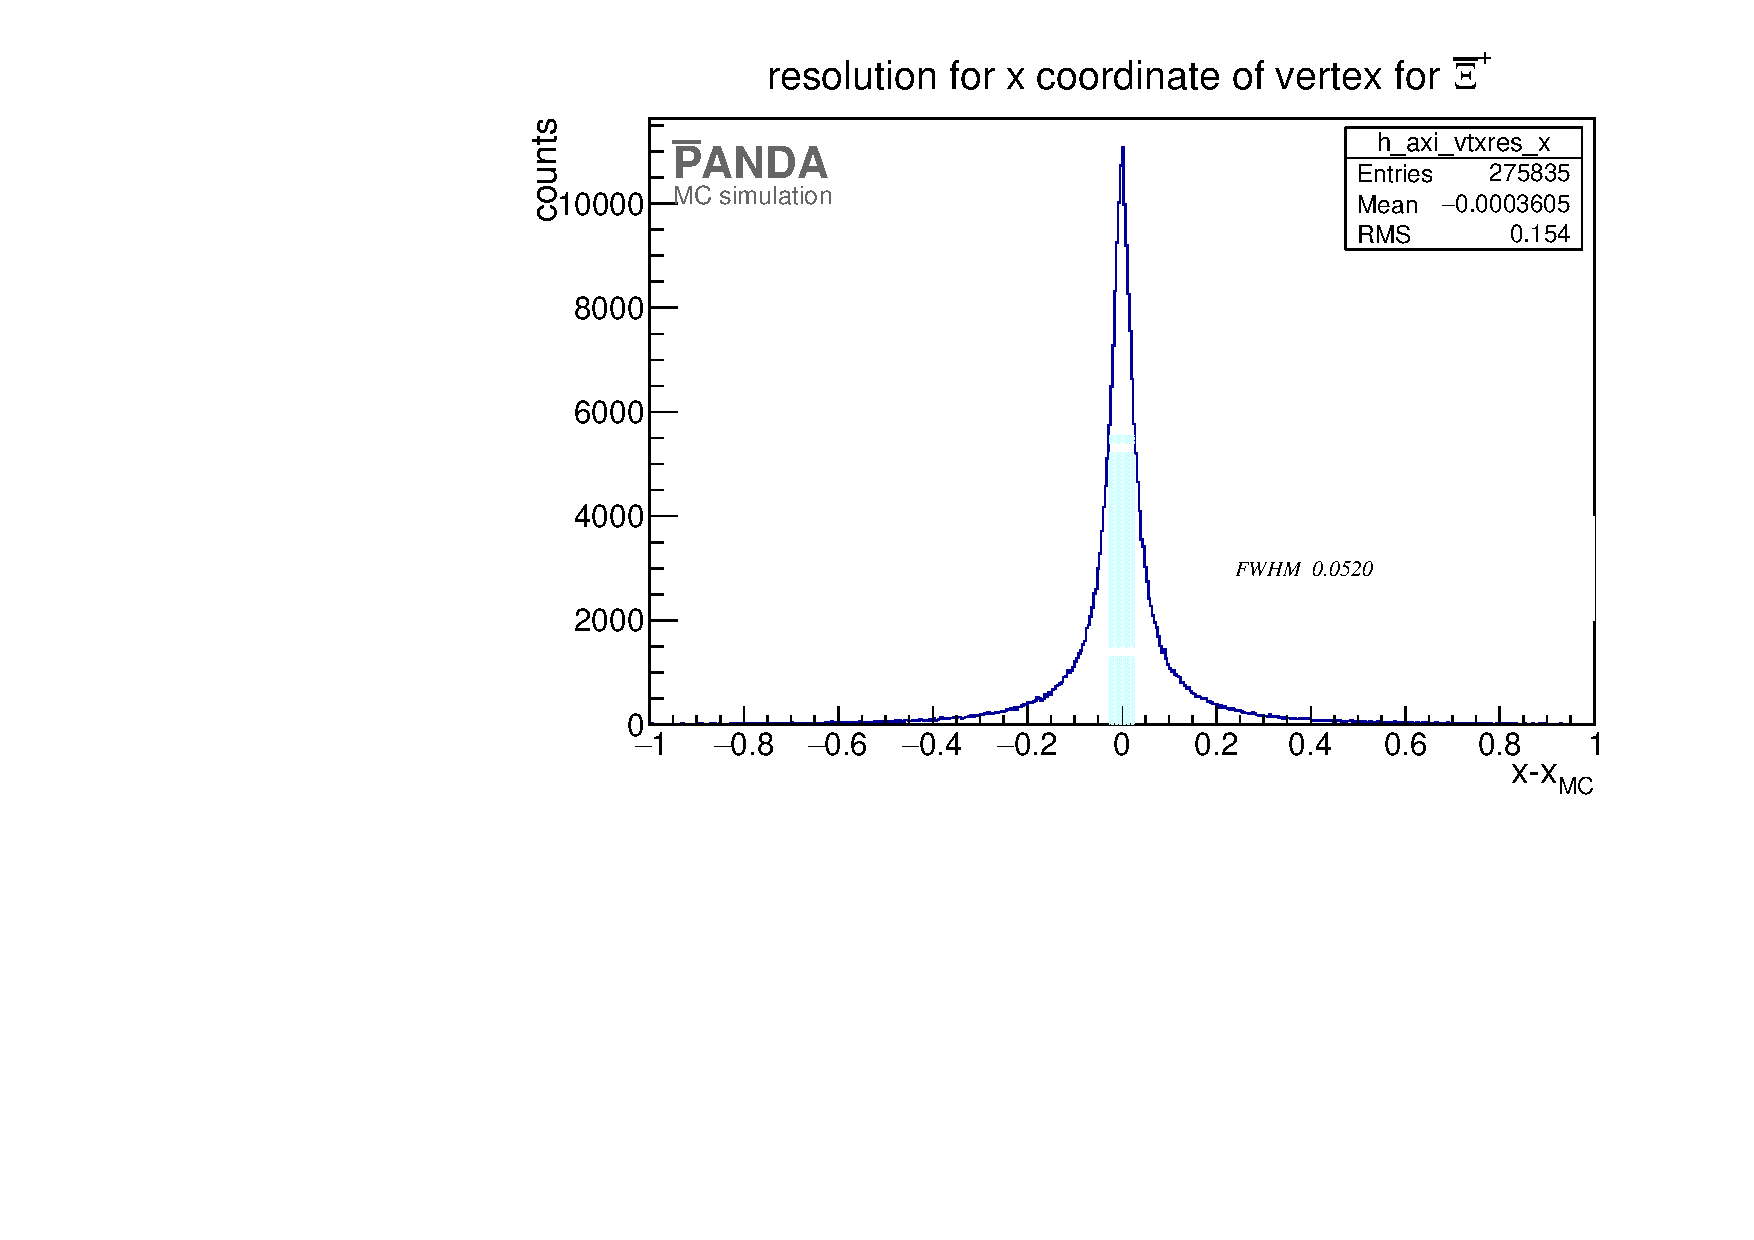
\includegraphics[width=0.8\textwidth]{./plots/Xi/XiPlus_vtxres_x.pdf}
			\caption{Vertex resolution of x position for \anticascade}
			\label{fig:xi_vtxres_x}
			
		\end{figure}
		
		\begin{figure}
			\subfigure[Vertex resolution for y coordinate]{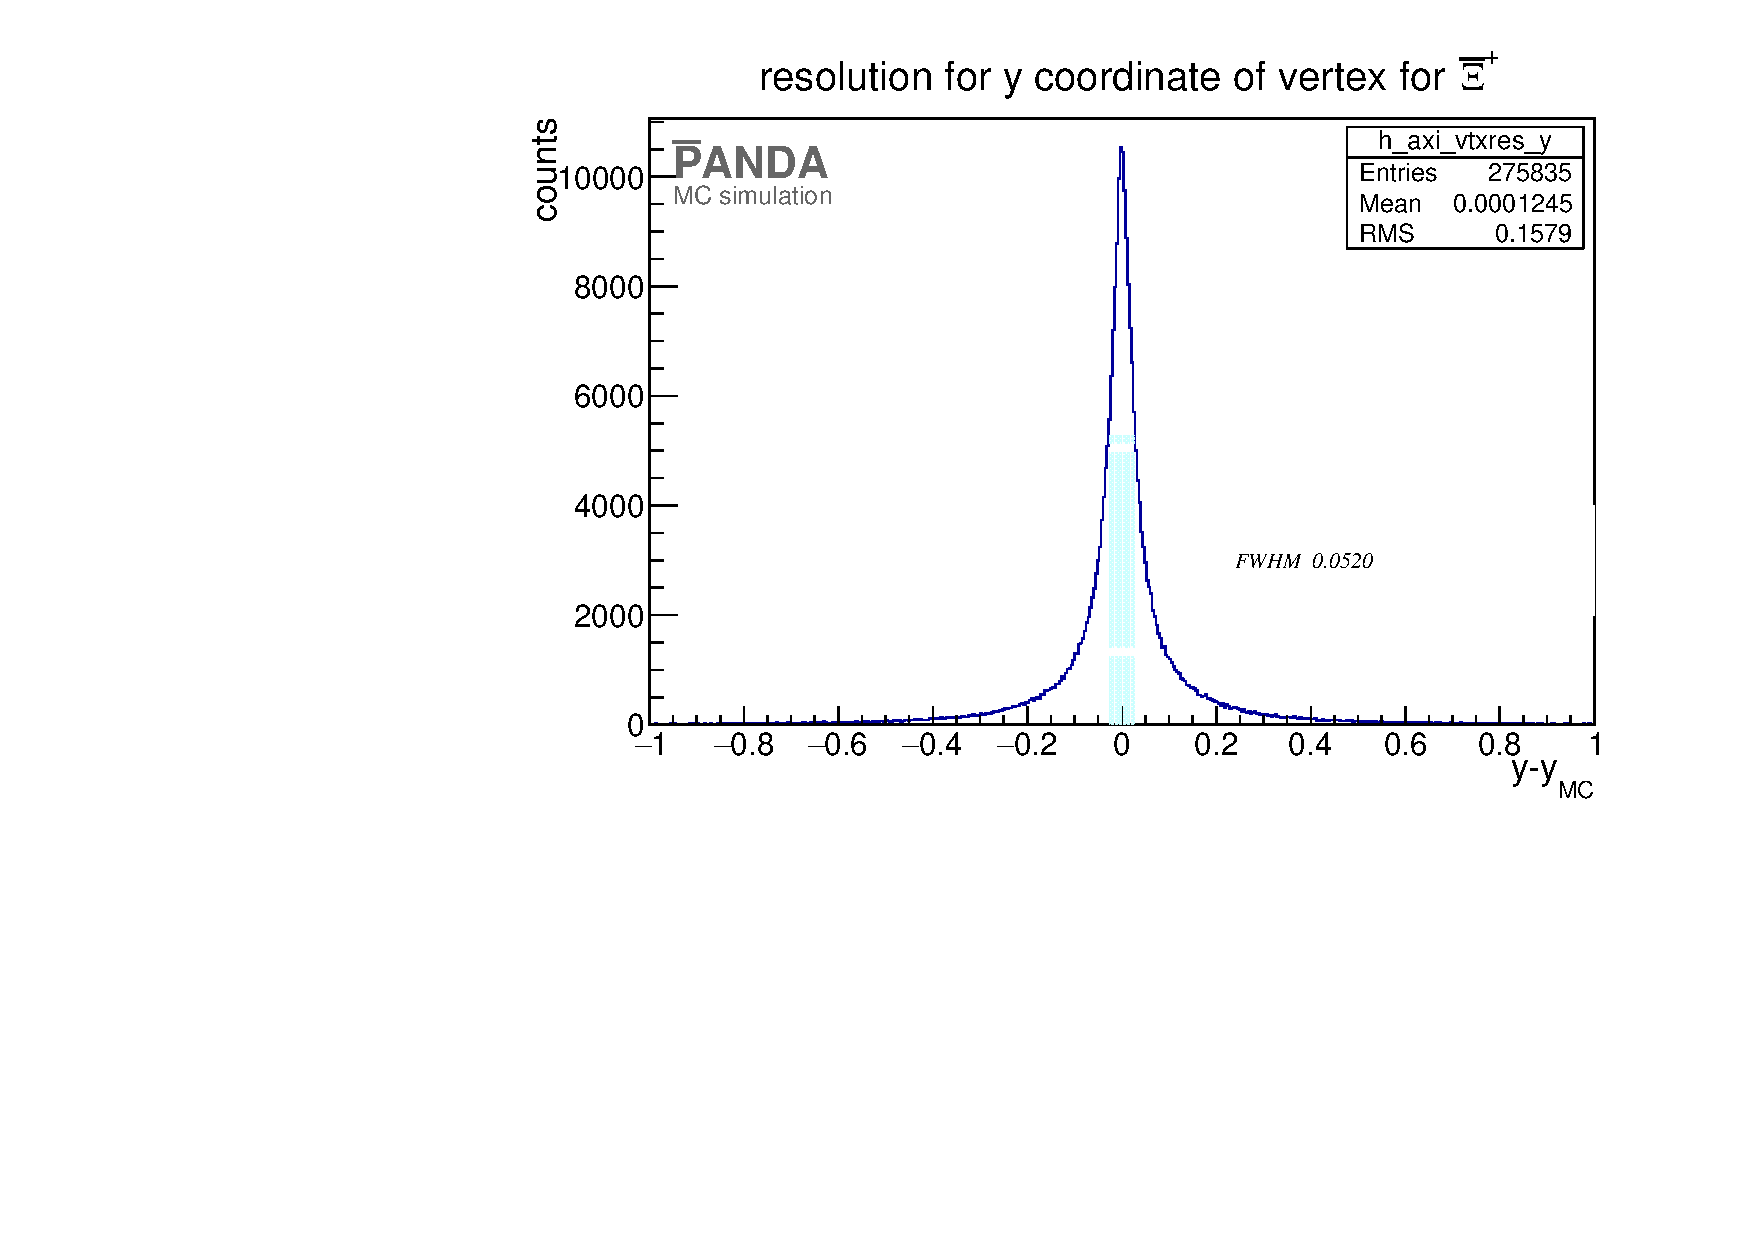
\includegraphics[width=0.49\textwidth]{./plots/Xi/XiPlus_vtxres_y.pdf}}
			\subfigure[Vertex resolution for z coordinate]{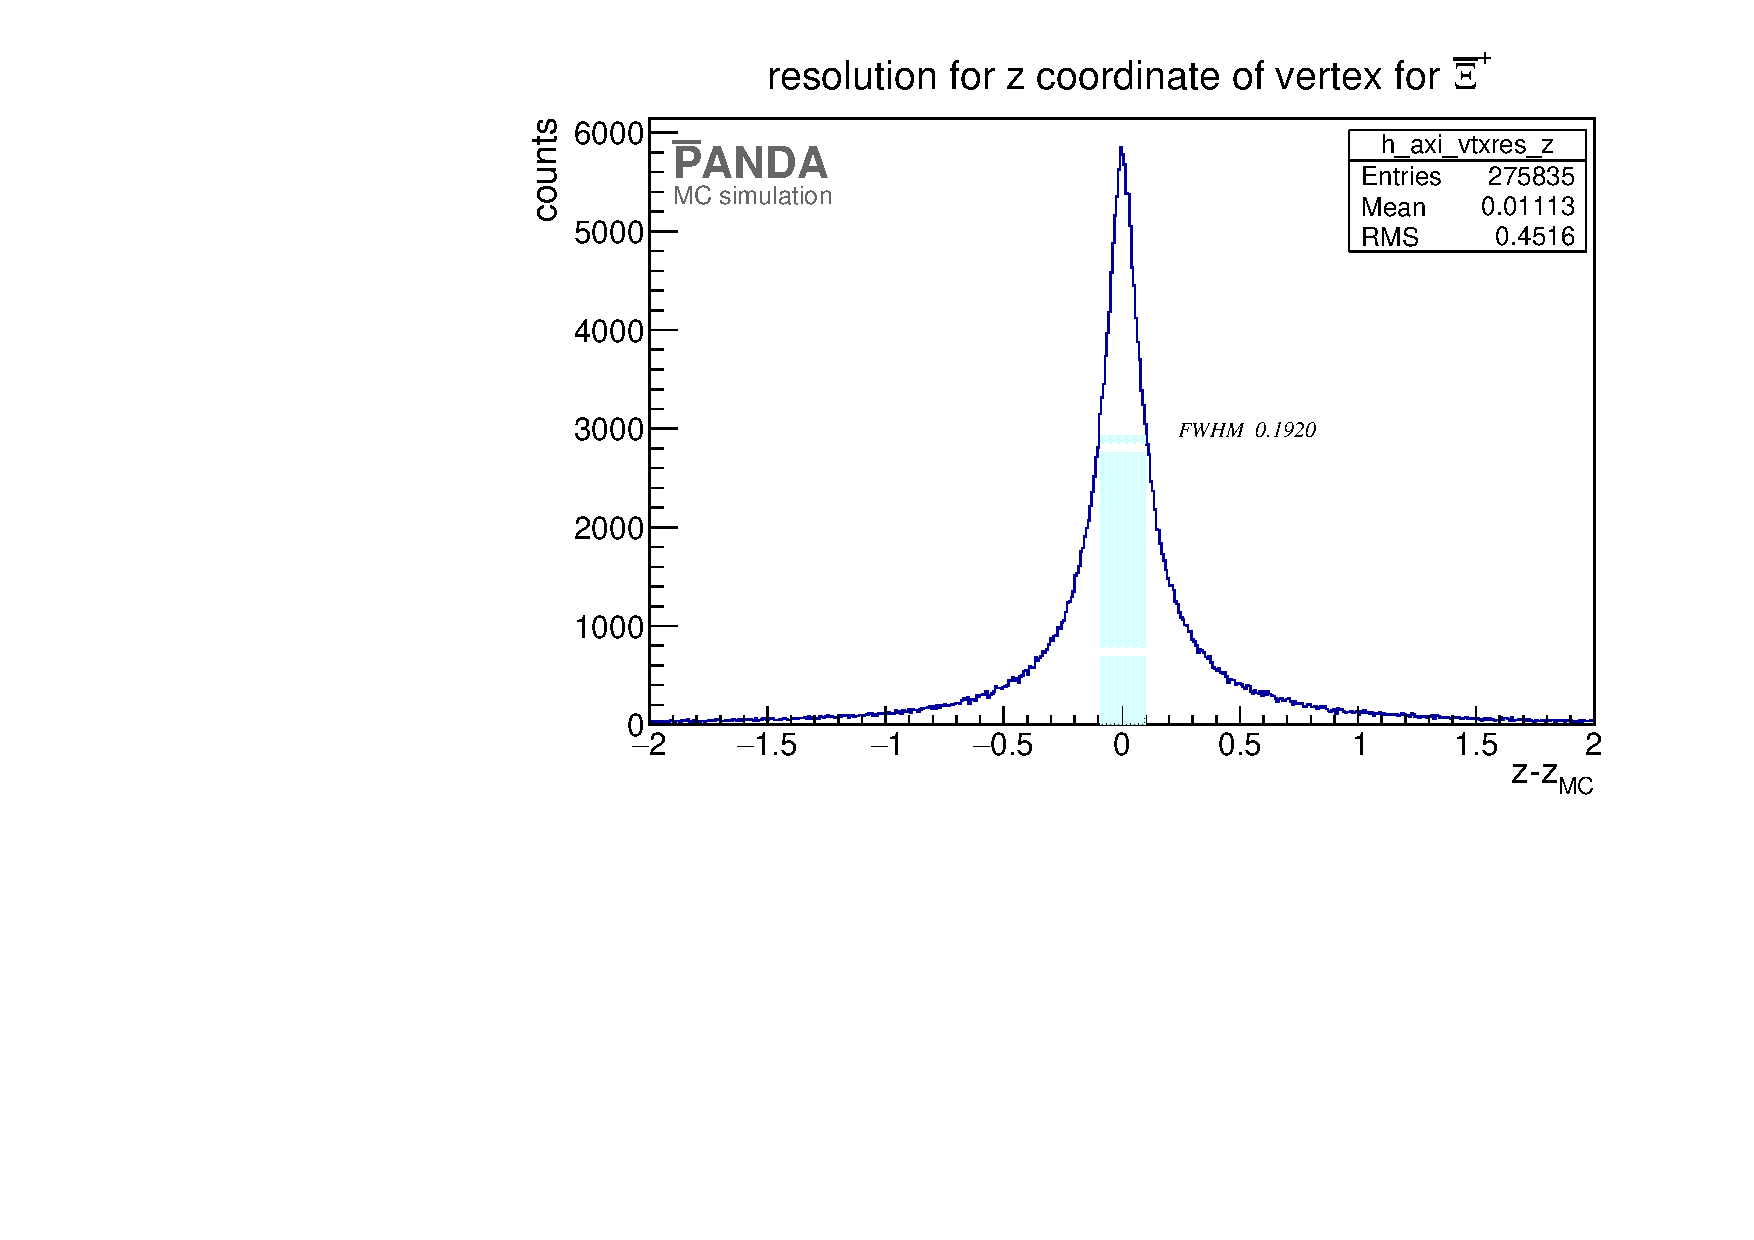
\includegraphics[width=0.49\textwidth]{./plots/Xi/XiPlus_vtxres_z.pdf}}
			\caption{left plot: Vertex resolution of y position for \anticascade; right plot: Vertex resolution of z position for \anticascade.}
			\label{fig:xi_vtxres_yz}
			
		\end{figure}
	
		The mass distribution for the different cuts is shown in figure \ref{fig:XiPlus_massdiffcuts} and figure \ref{fig:XiMinus_massdiffcuts}. 
		The vertex fitter cut reduces the number of events most and the width of the mass distribution gets smaller.
		
		\begin{figure}
			\centering
				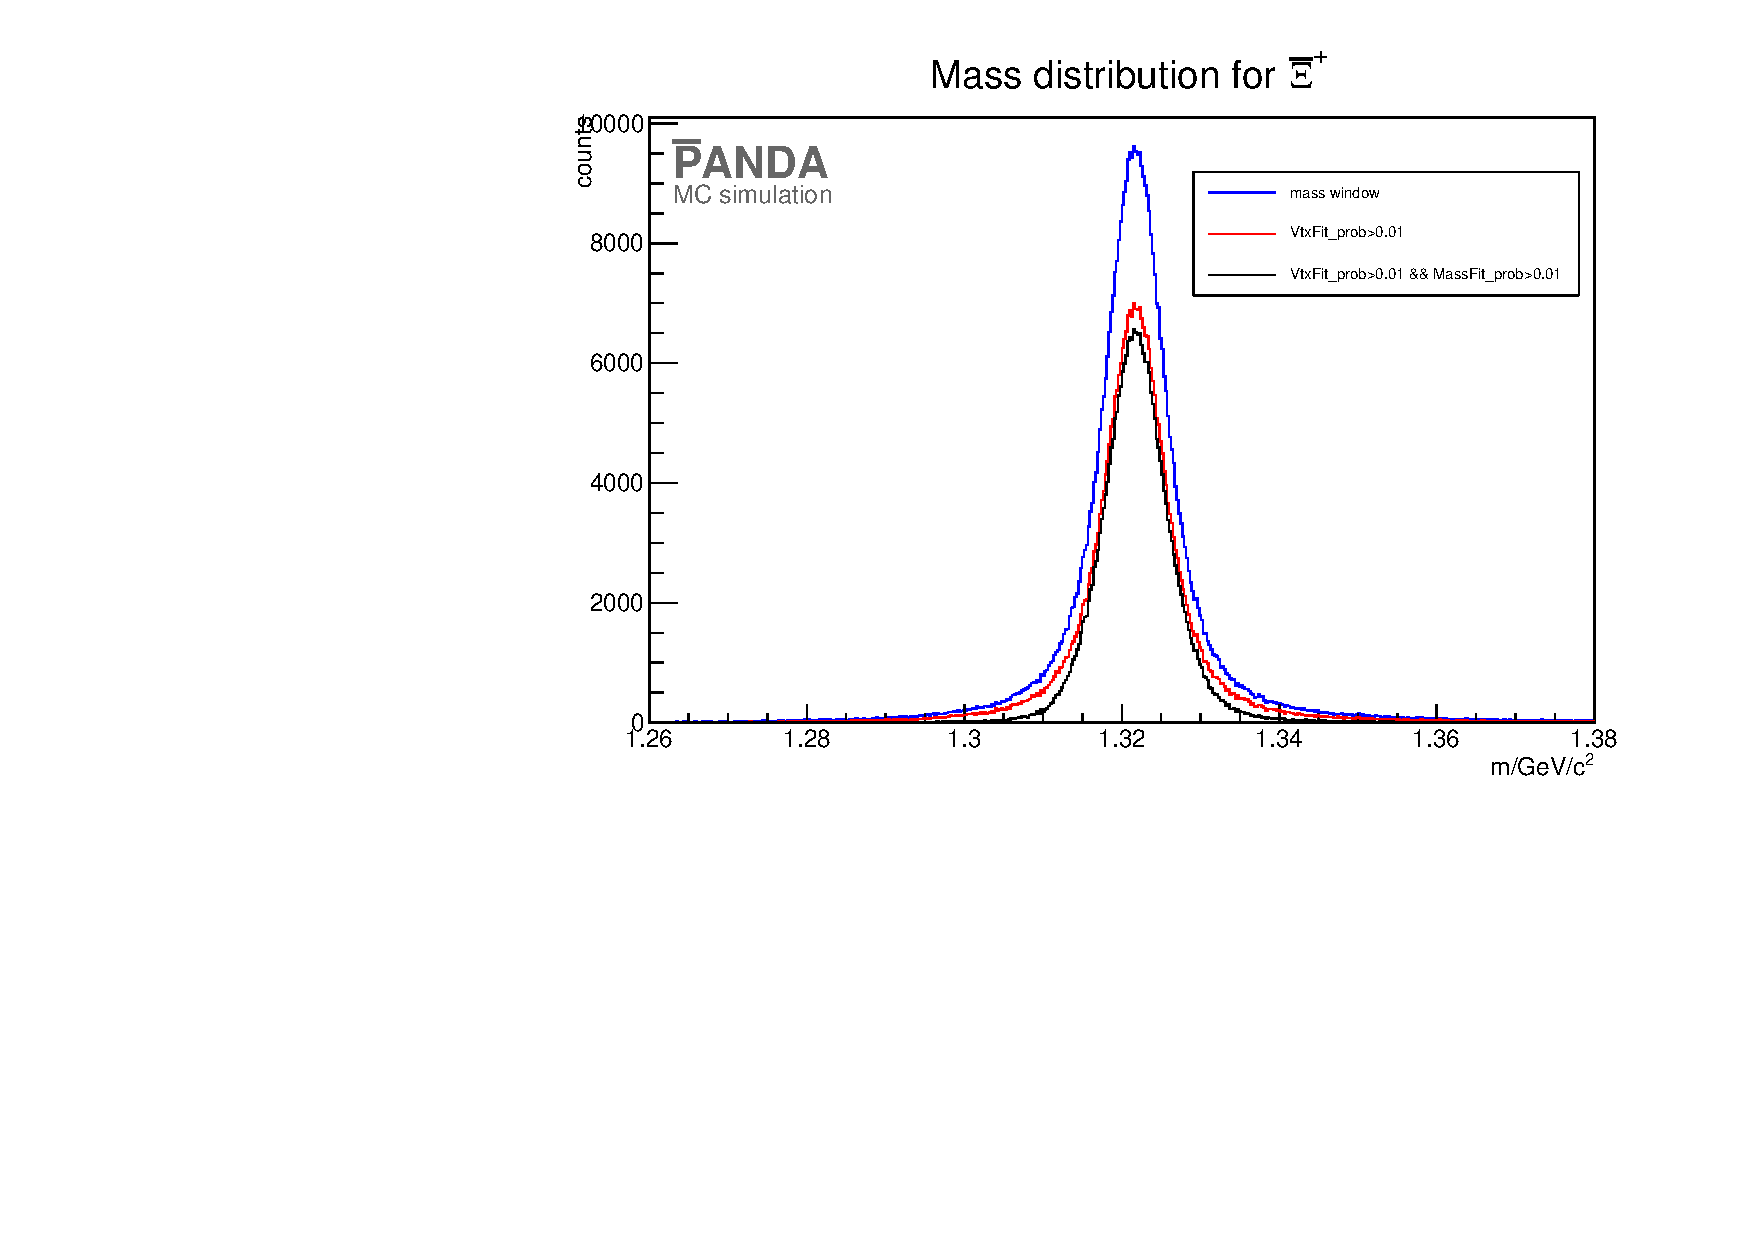
\includegraphics[width=1.1\textwidth]{./plots/Xi/XiPlus_m_diffcuts.pdf}
			\caption{Mass distribution of \anticascade for different cuts}
			\label{fig:XiPlus_massdiffcuts}
			
				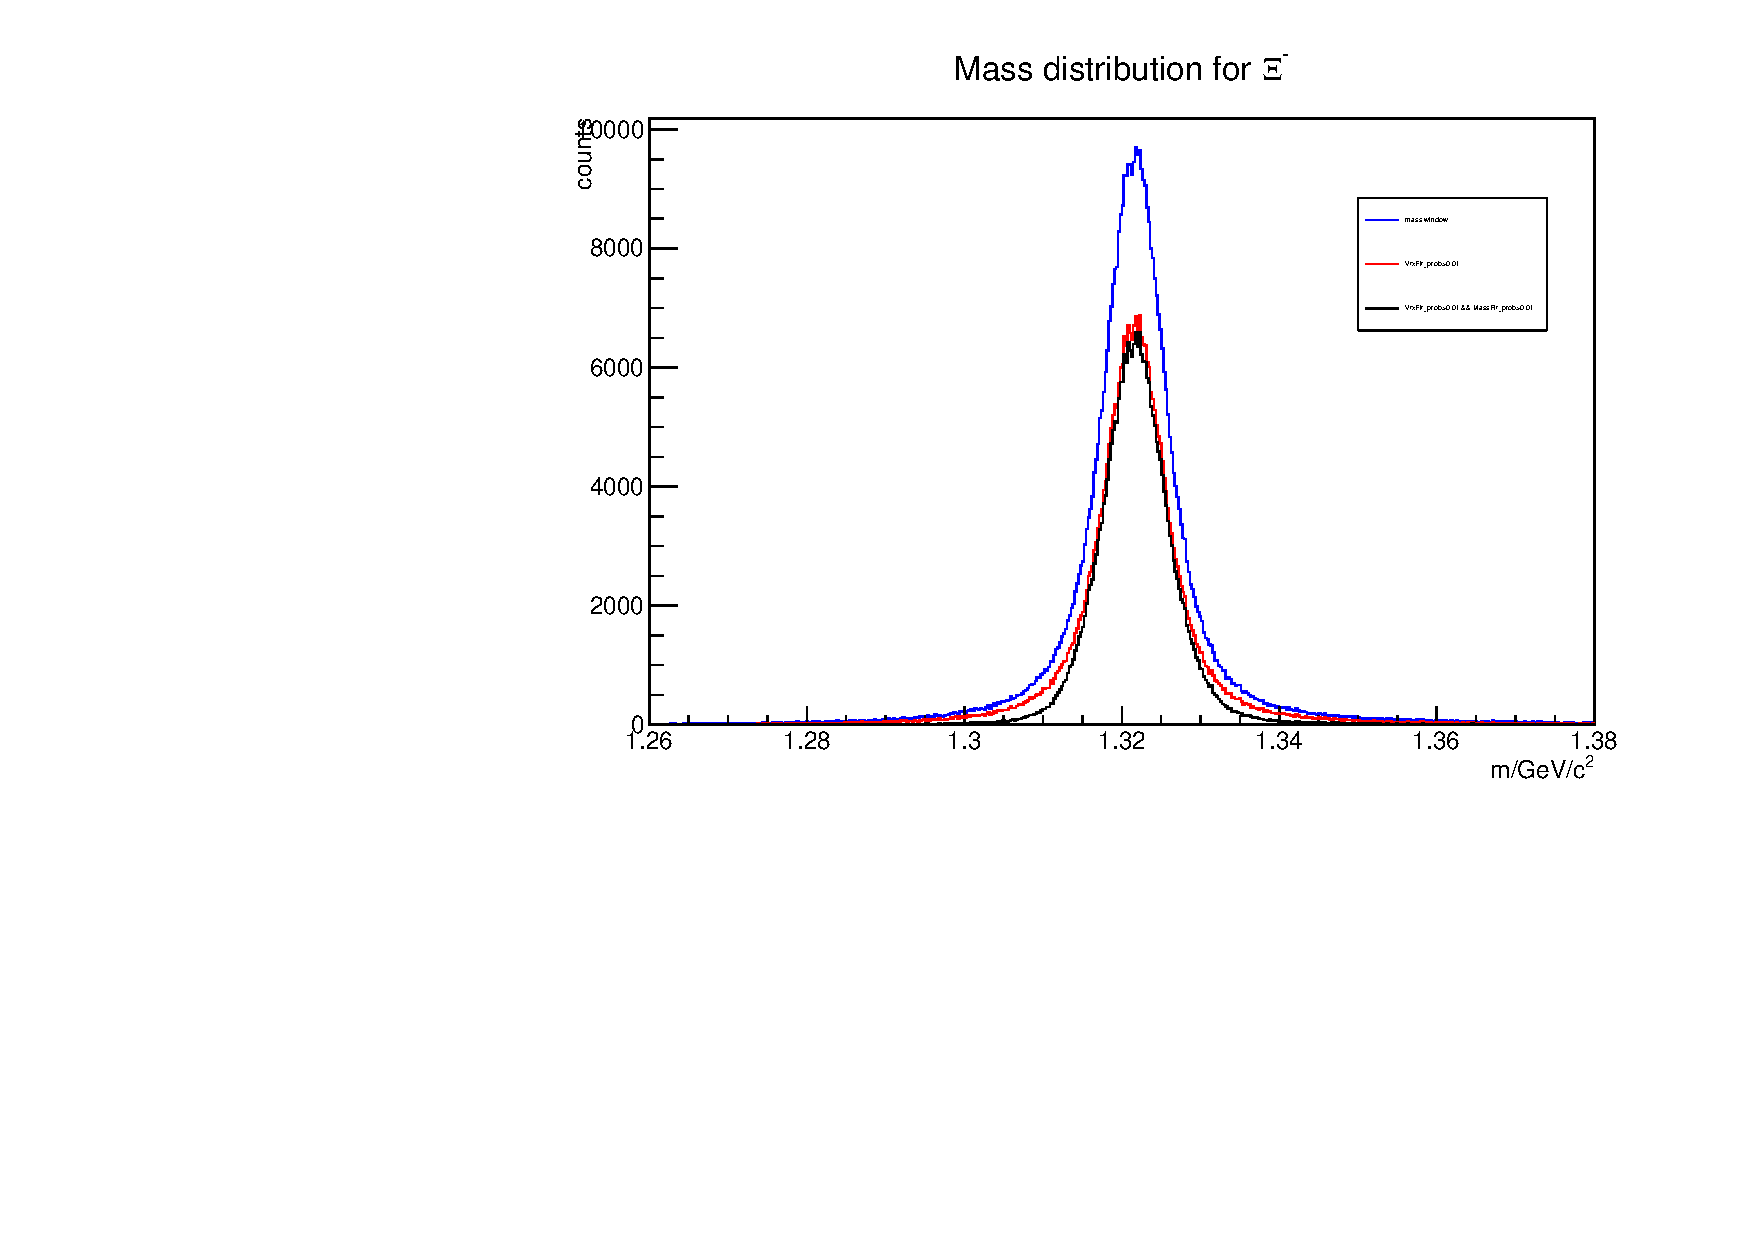
\includegraphics[width=1.1\textwidth]{./plots/Xi/XiMinus_m_diffcuts.pdf}
			\caption{Mass distribution of \cascade for different cuts}
			\label{fig:XiMinus_massdiffcuts}
		\end{figure}
		
		After using all cuts on the mass distribution the reconstructed mass of \cascade and \anticascade can be determined by a double Gaussian fit.
		This is exemplarily shown for the \cascade in figure \ref{fig:XiPlus_massfit}.
		
		\begin{figure}
			\centering
				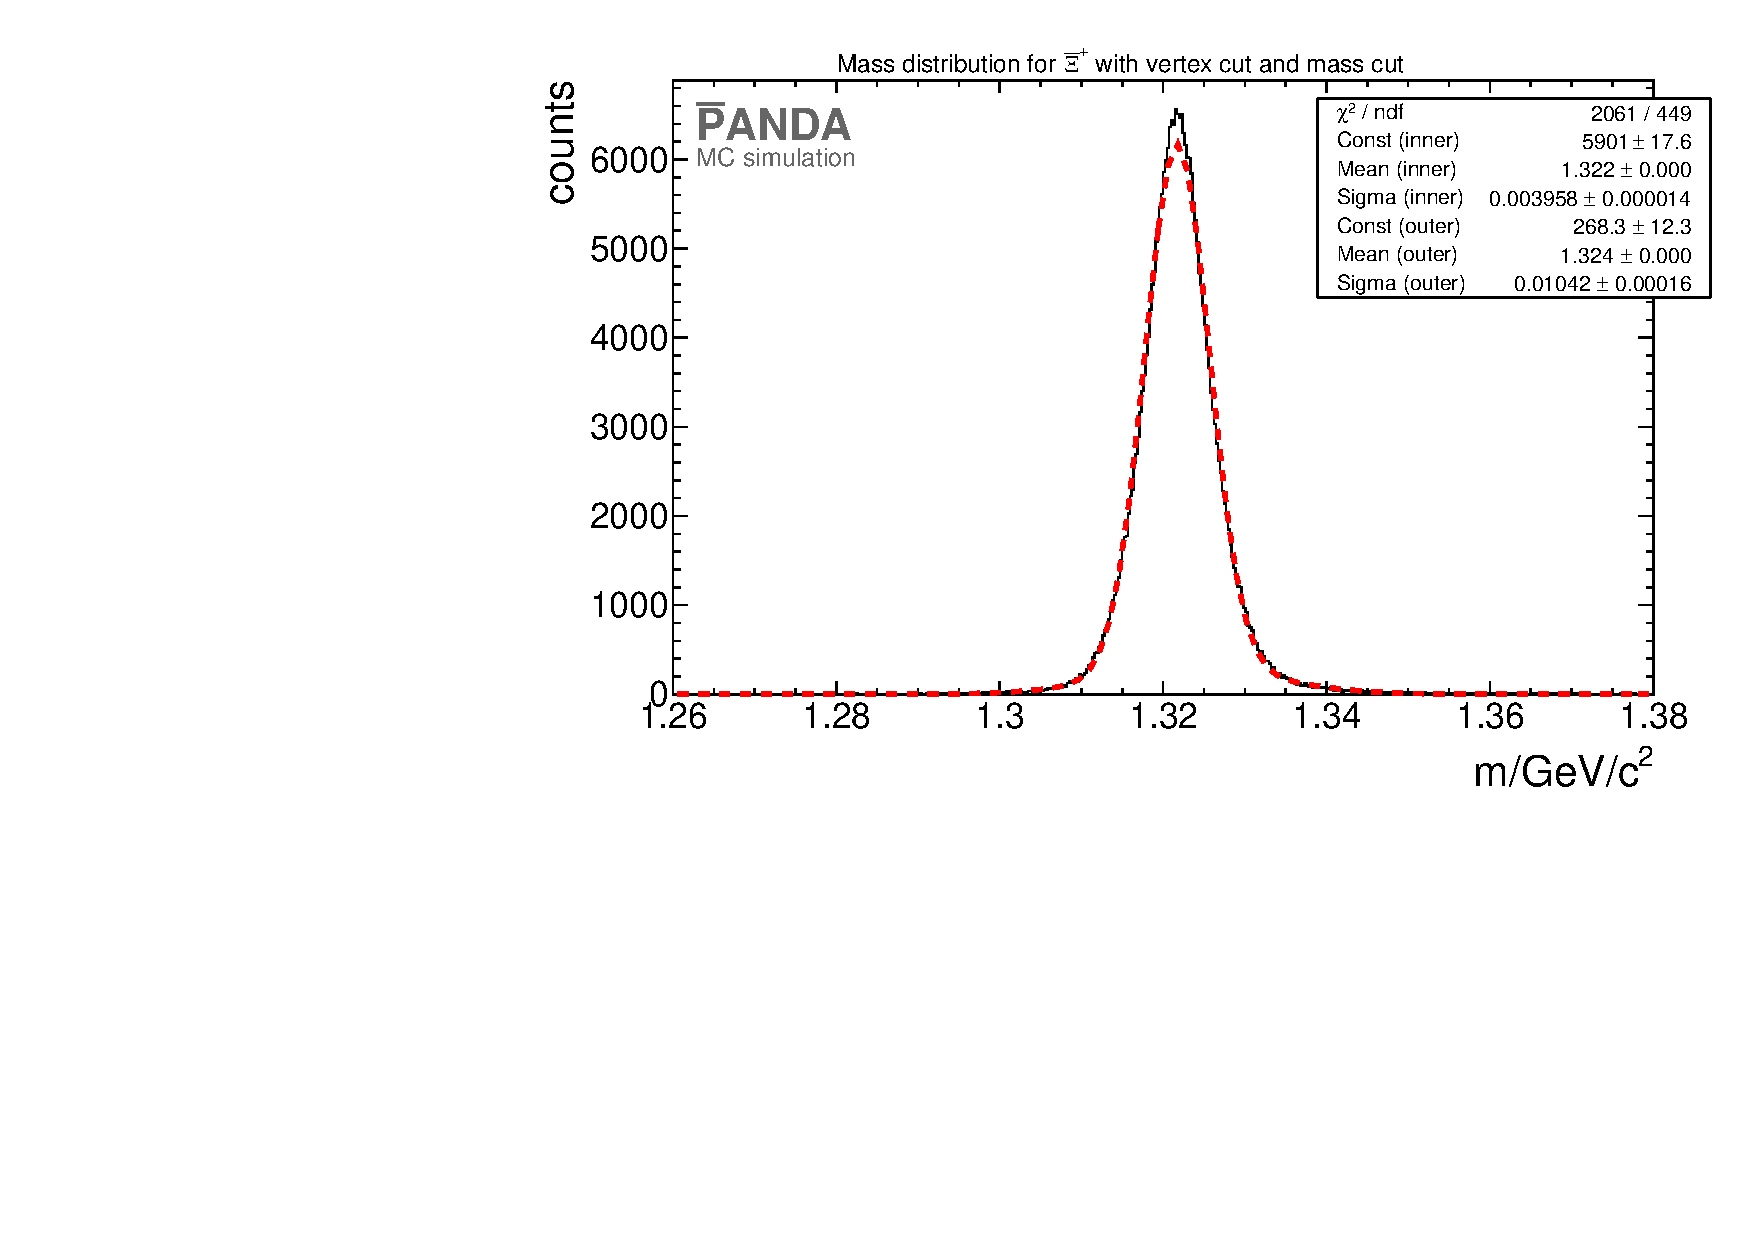
\includegraphics[width=0.8\textwidth]{./plots/Xi/XiPlus_m_masscut.pdf}
			\caption{Mass fit with a double gaussian fit}
			\label{fig:XiPlus_massfit}
		\end{figure}
		The result of the mass fit is for \anticascade $\mt{m} = \left( 1.3721716 \pm 9.2\cdot 10^{-5}\right)$ \massunit 
		and for \cascade $\mt{m} = \left( 1\pm 1\cdot 10^{-5}\right)$ \massunit.
		The two dimensional momentum distribution for \anticascade and \cascade is shown in figure \ref{fig:XiPlus_pt_vs_pz} 
		
		\begin{figure}
			\subfigure[\anticascade]{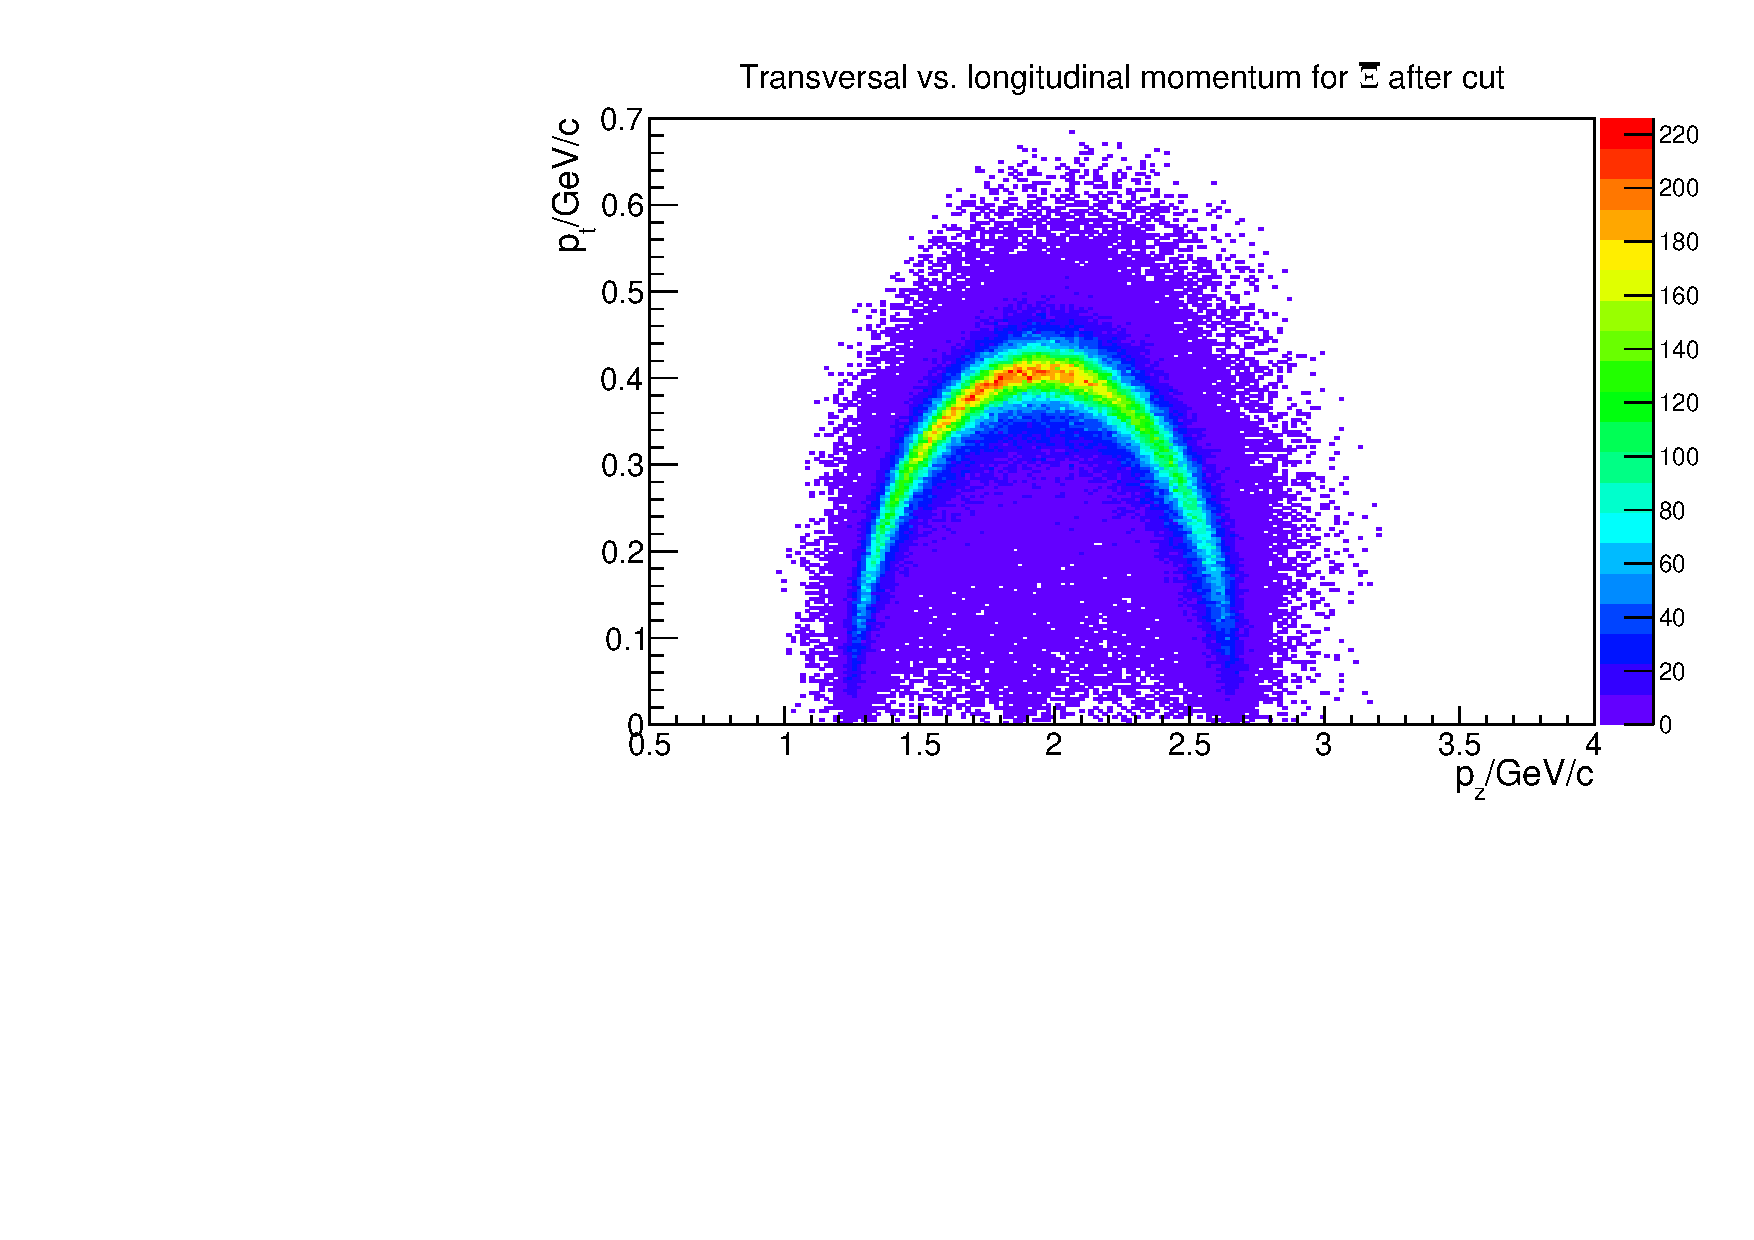
\includegraphics[width=0.49\textwidth]{./plots/Xi/XiPlus_pt_vs_pz_cut.pdf}}
			\subfigure[\cascade]{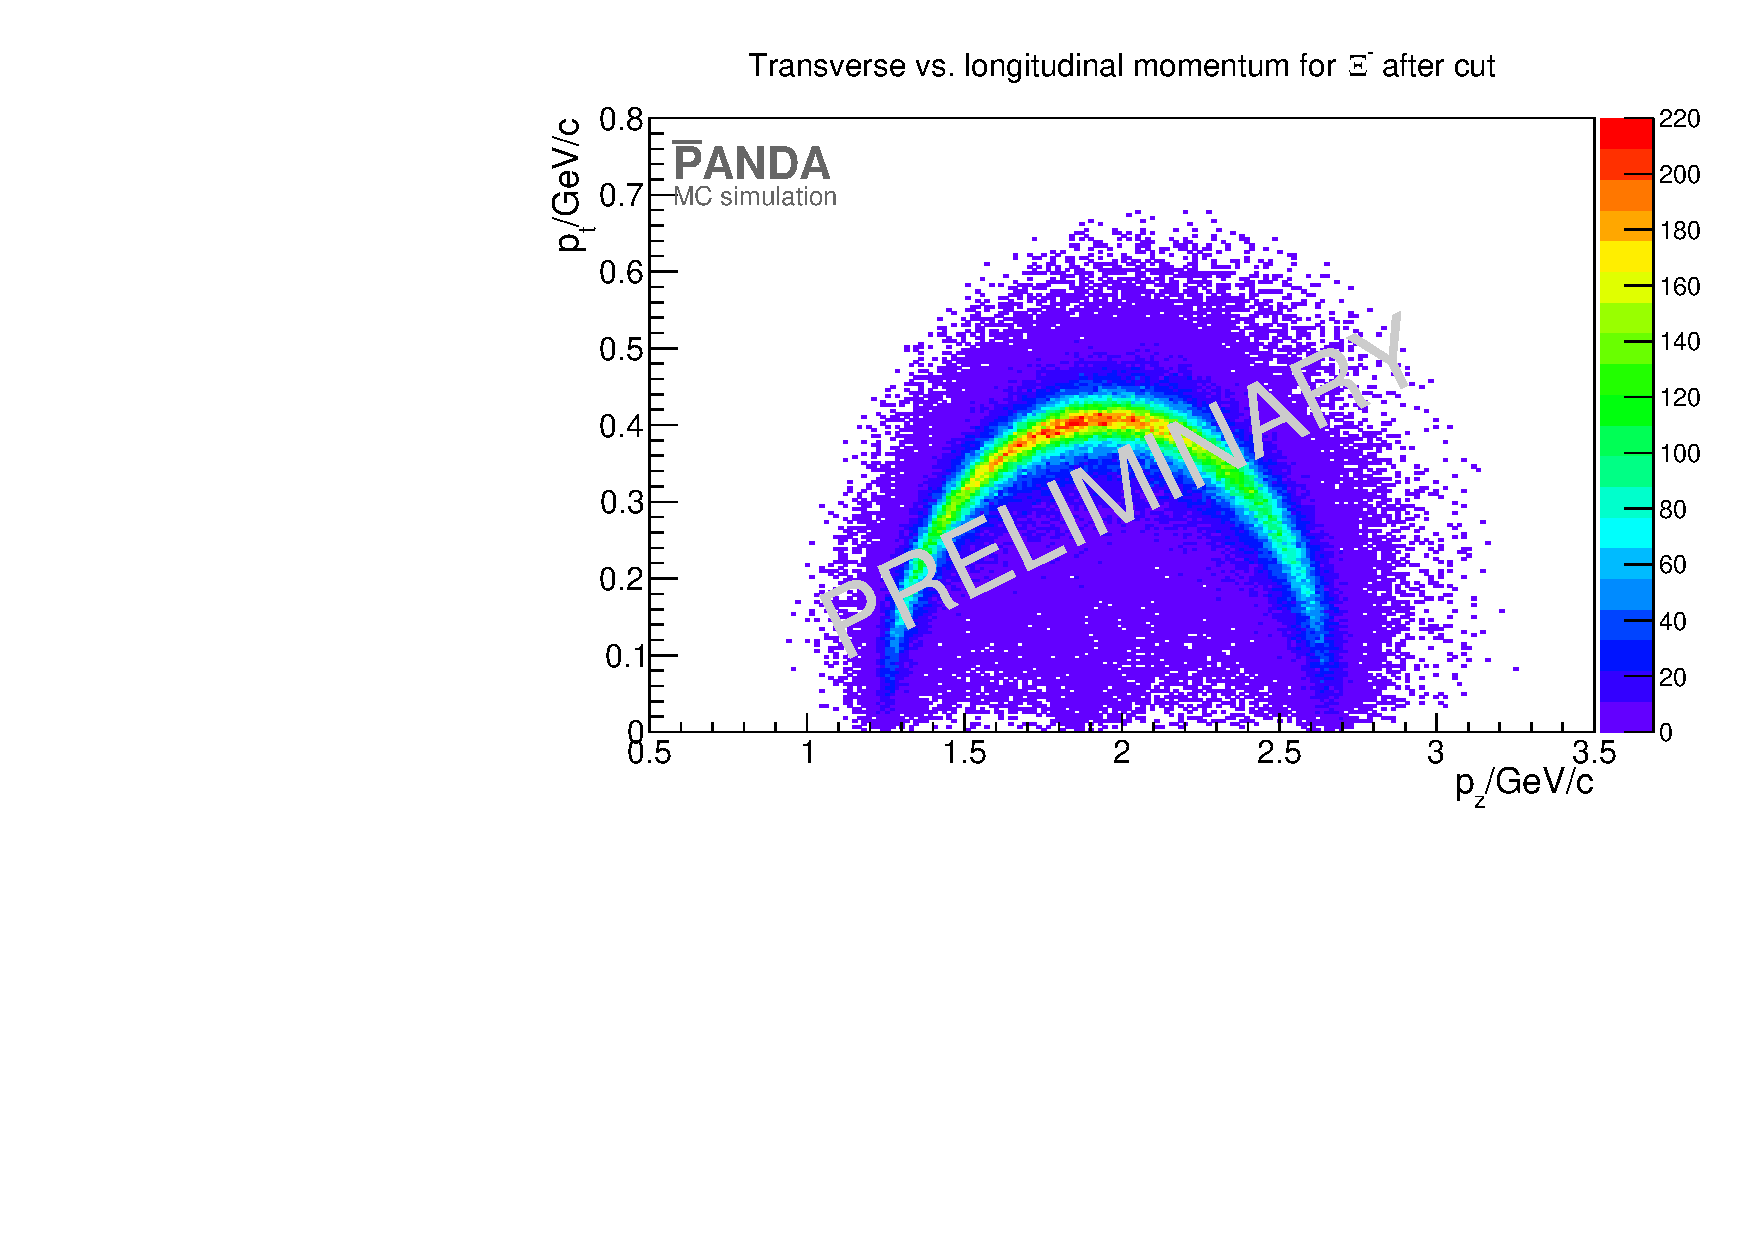
\includegraphics[width=0.49\textwidth]{./plots/Xi/XiMinus_pt_vs_pz_cut.pdf}}
			\caption{The plots shows the transverse against the longuitudinal momentum for \anticascade and \cascade}
			\label{fig:XiPlus_pt_vs_pz}
		
		\end{figure}
		
		The reconstruction efficiency for \anticascade is $18.39\%$ and for \cascade $18.64\%$.
		
	
	
	

\section{Reconstruction of $\boldmath{\Xi}$(1820) and $\boldmath{\bar{\Xi}}$(1820)}
		\subsection*{Selection}

		For the reconstruction of \excitedcascade one combine \lam and \kminus meson and for \excitedanticascade \alam and \kplus using the
		best candidate from \lam and \alam and \kplus and \kminus with more than 3 hits in one of the inner tracking detectors.
		After the combination of the particles a mass window cut with width of $0.3$\massunit is performed. 
		The daughter particles are fitted then to a common vertex point with the PndKinVtxFitter.
		Only those candidates for \excitedcascade (\excitedanticascade) are selected which have a fit probability of more then $1\%$.
		The selection scheme is shown in figure \ref{fig:excitedcascade_scheme}. 
		
		\begin{figure}
			\centering
				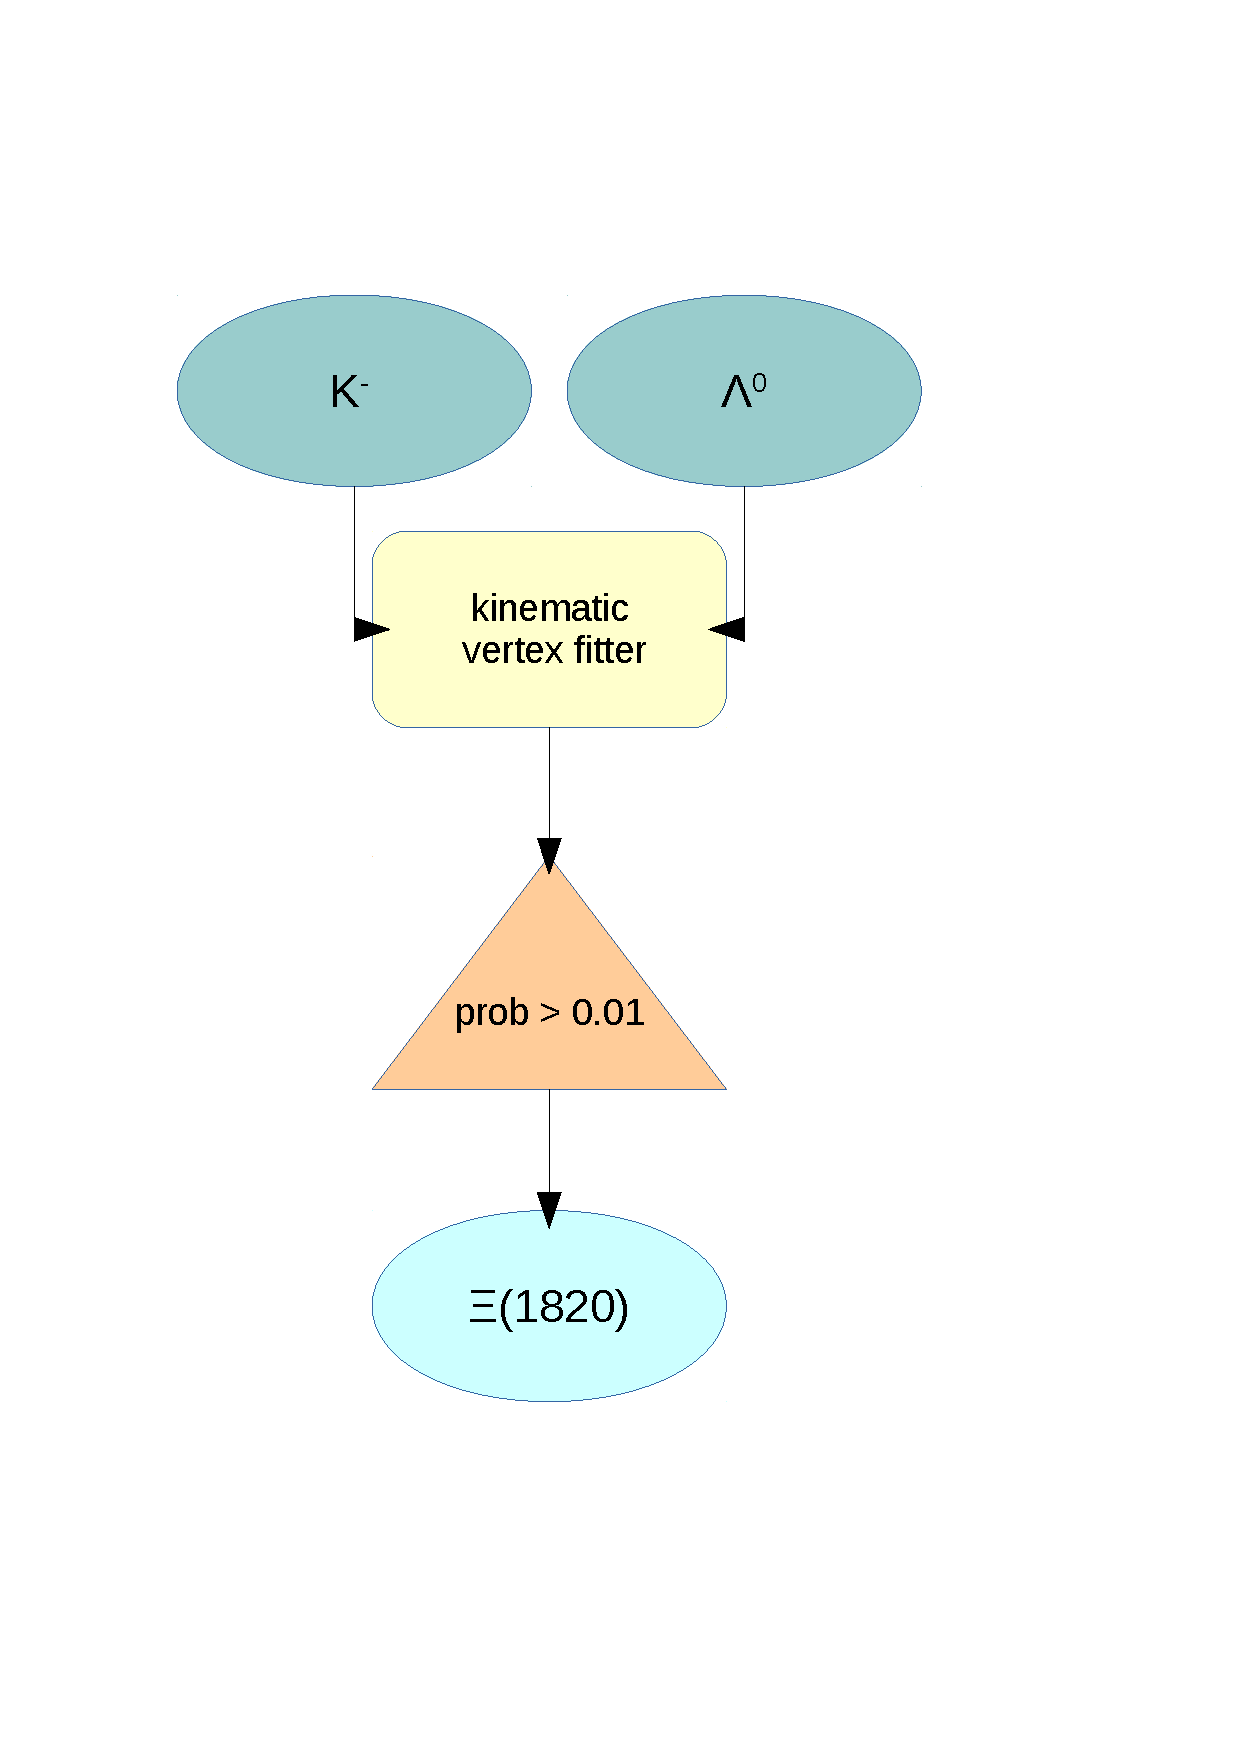
\includegraphics[width=0.50\textwidth]{./plots/combineExcitedCascade.pdf}
			\caption{Scheme for \excitedcascade reconstruction}
			\label{fig:excitedcascade_scheme}
		\end{figure}
		
		
		The \chisq probability distribution for the vertex fit is shown in figure \ref{fig:xi1820_prob}.
		The distribution is again not flat but increases for values up to one. 
		
		\begin{figure}
			\centering
			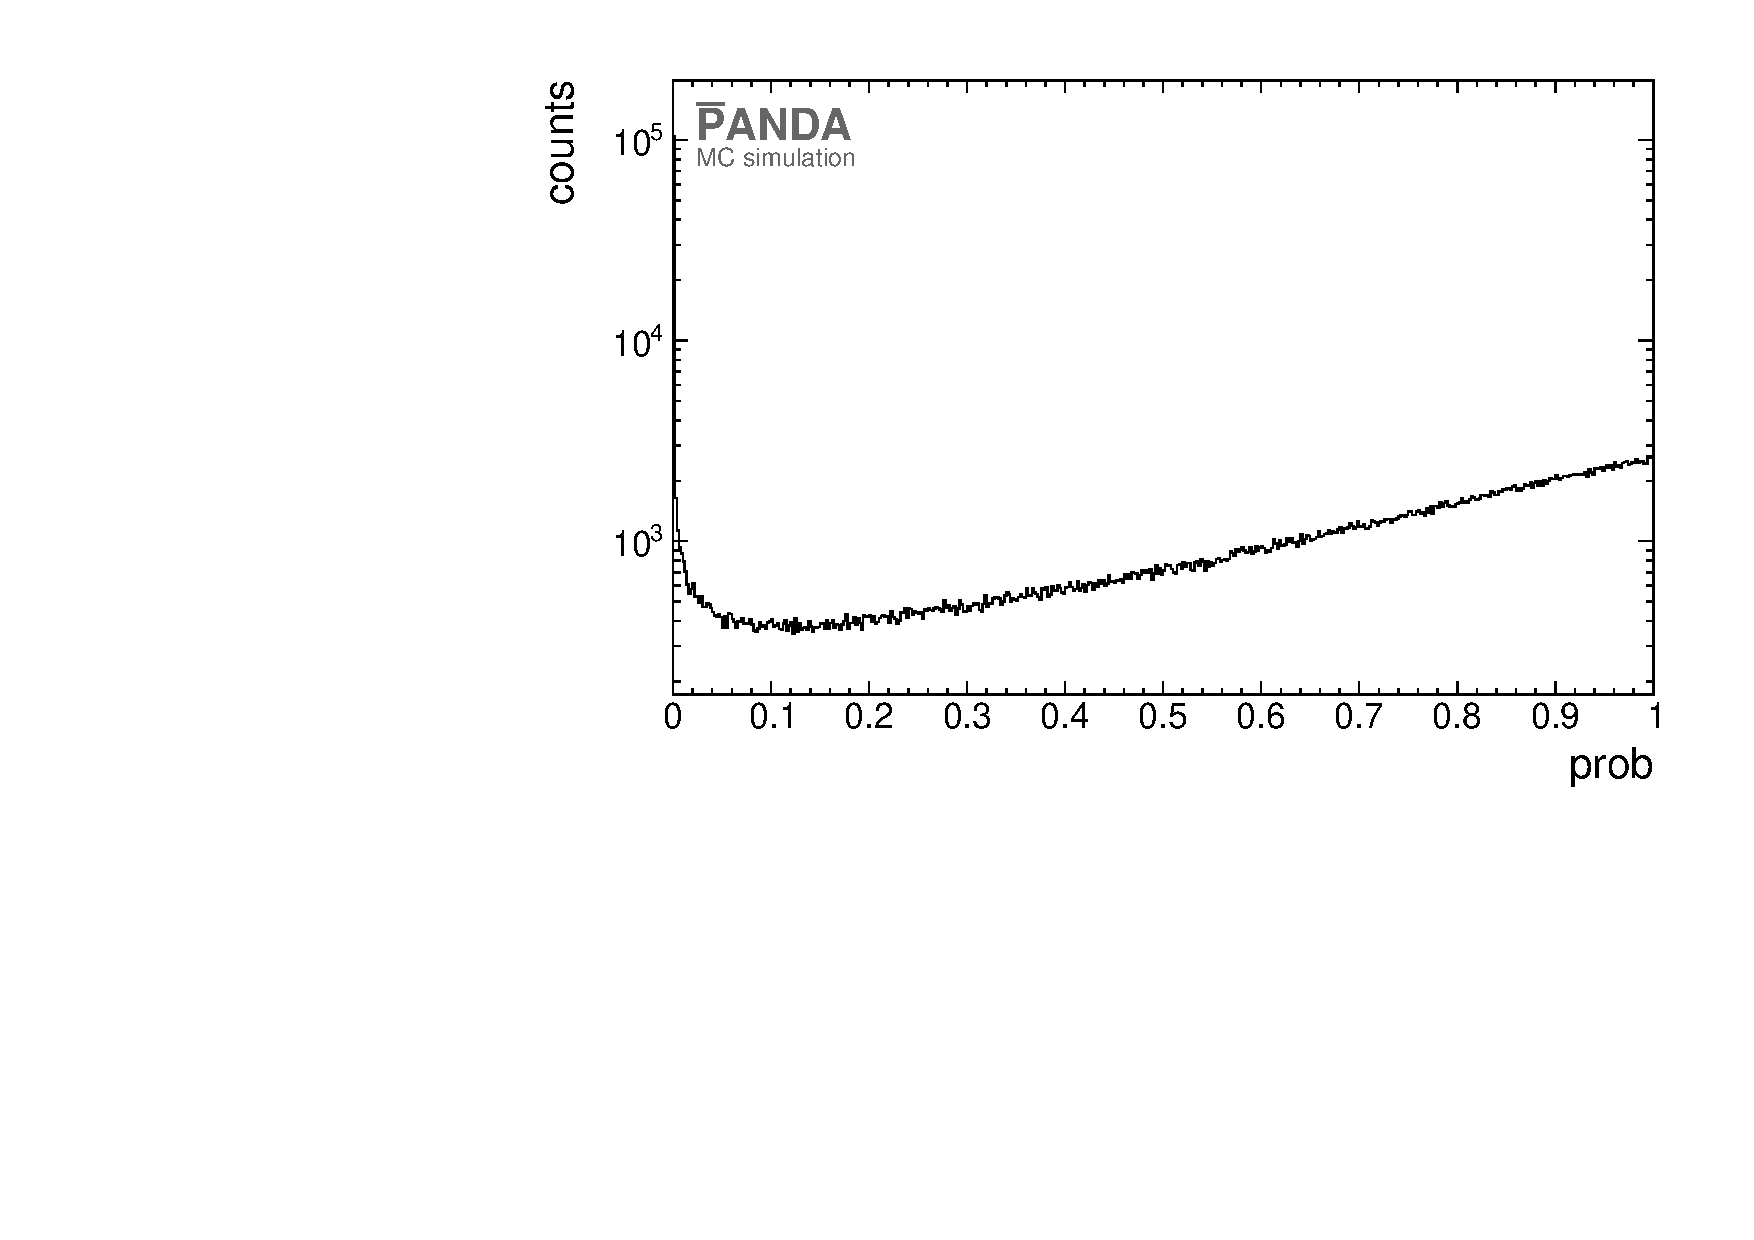
\includegraphics[width=1.\textwidth]{./plots/Xi1820/XiMinus1820_prob.pdf}
			\caption{\chisq probability distribution of kinematic vertex fit for \excitedcascade.}
			\label{fig:xi1820_prob}
		\end{figure}
		
		If there is more than one particle the best candidate is chosen.
		
	\subsection*{Results}
	The vertex resolution for \excitedcascade and \excitedanticascade is summarized in table \ref{tab:Xi1820_vtxres}.
	
	\begin{table}
		\centering
		\caption{Vertex resolution for \excitedcascade and \excitedanticascade.}
		\label{tab:Xi1820_vtxres}
		\begin{tabular}{ccc}
			\hline
			position & \excitedcascade & \excitedanticascade (from c.c.) \\
			\hline
			\hline
			x/cm & 0.028 & 0.028\\
			y/cm & 0.028 & 0.028\\
			z/cm & 0.1 & 0.1\\
			\hline
			 
		\end{tabular}
	\end{table}
	
	Here again the vertex resolution is calculated with the FWHM. 
	This is exemplarily shown for \excitedcascade in figure \ref{fig:Xi1820_vtxx} and figure \ref{fig:Xi1820_vtxyz}.
	
	\begin{figure}
		\centering
		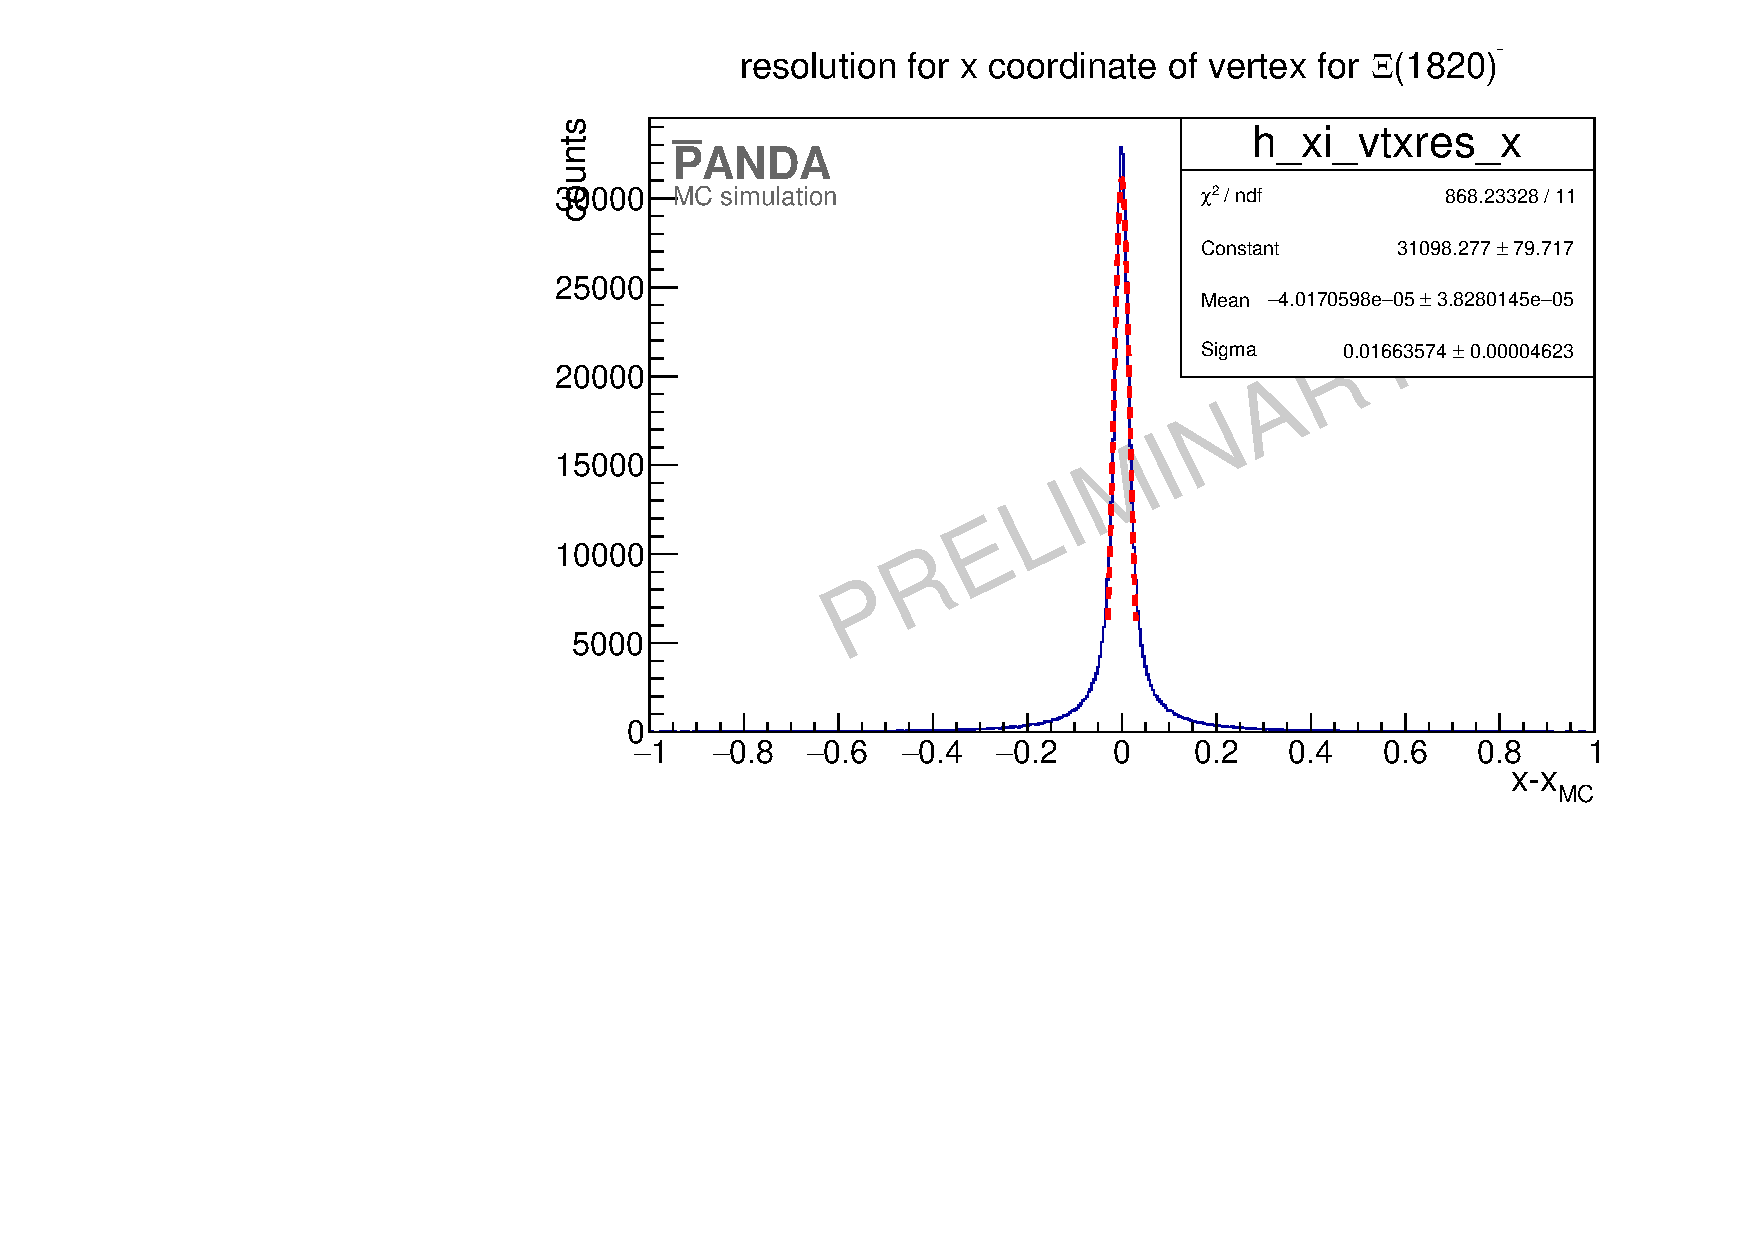
\includegraphics[width=0.7\textwidth]{./plots/Xi1820/XiMinus1820_vtxres_x.pdf}
		\caption{Vertex resolution of the x coordinate for \excitedcascade.}
		\label{fig:Xi1820_vtxx}
	\end{figure}
	
	 \begin{figure}
		\centering
		\subfigure[Vertex resolution of the y coordinate for \excitedcascade.]{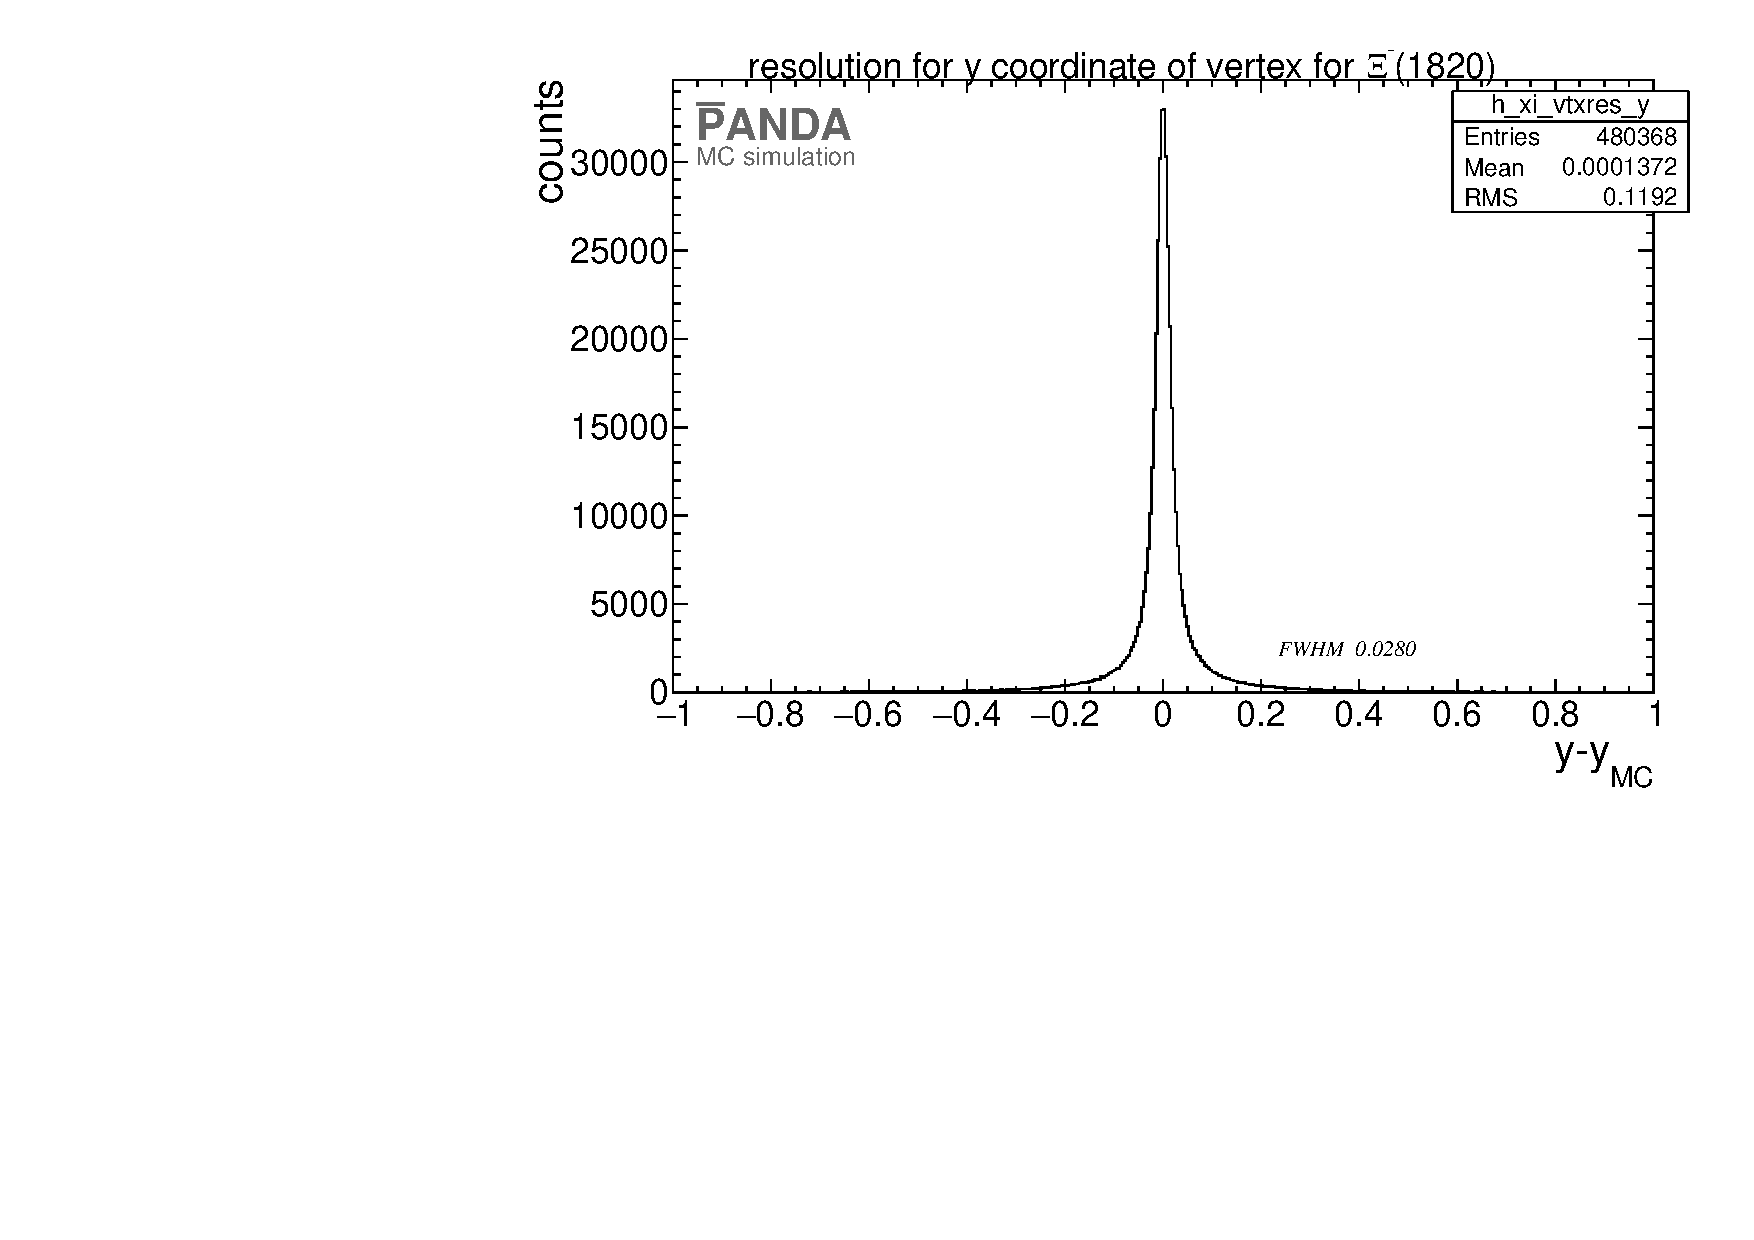
\includegraphics[width=0.49\textwidth]{./plots/Xi1820/XiMinus1820_vtxres_y.pdf}}
		\subfigure[Vertex resolution of the z coordinate for \excitedcascade.]{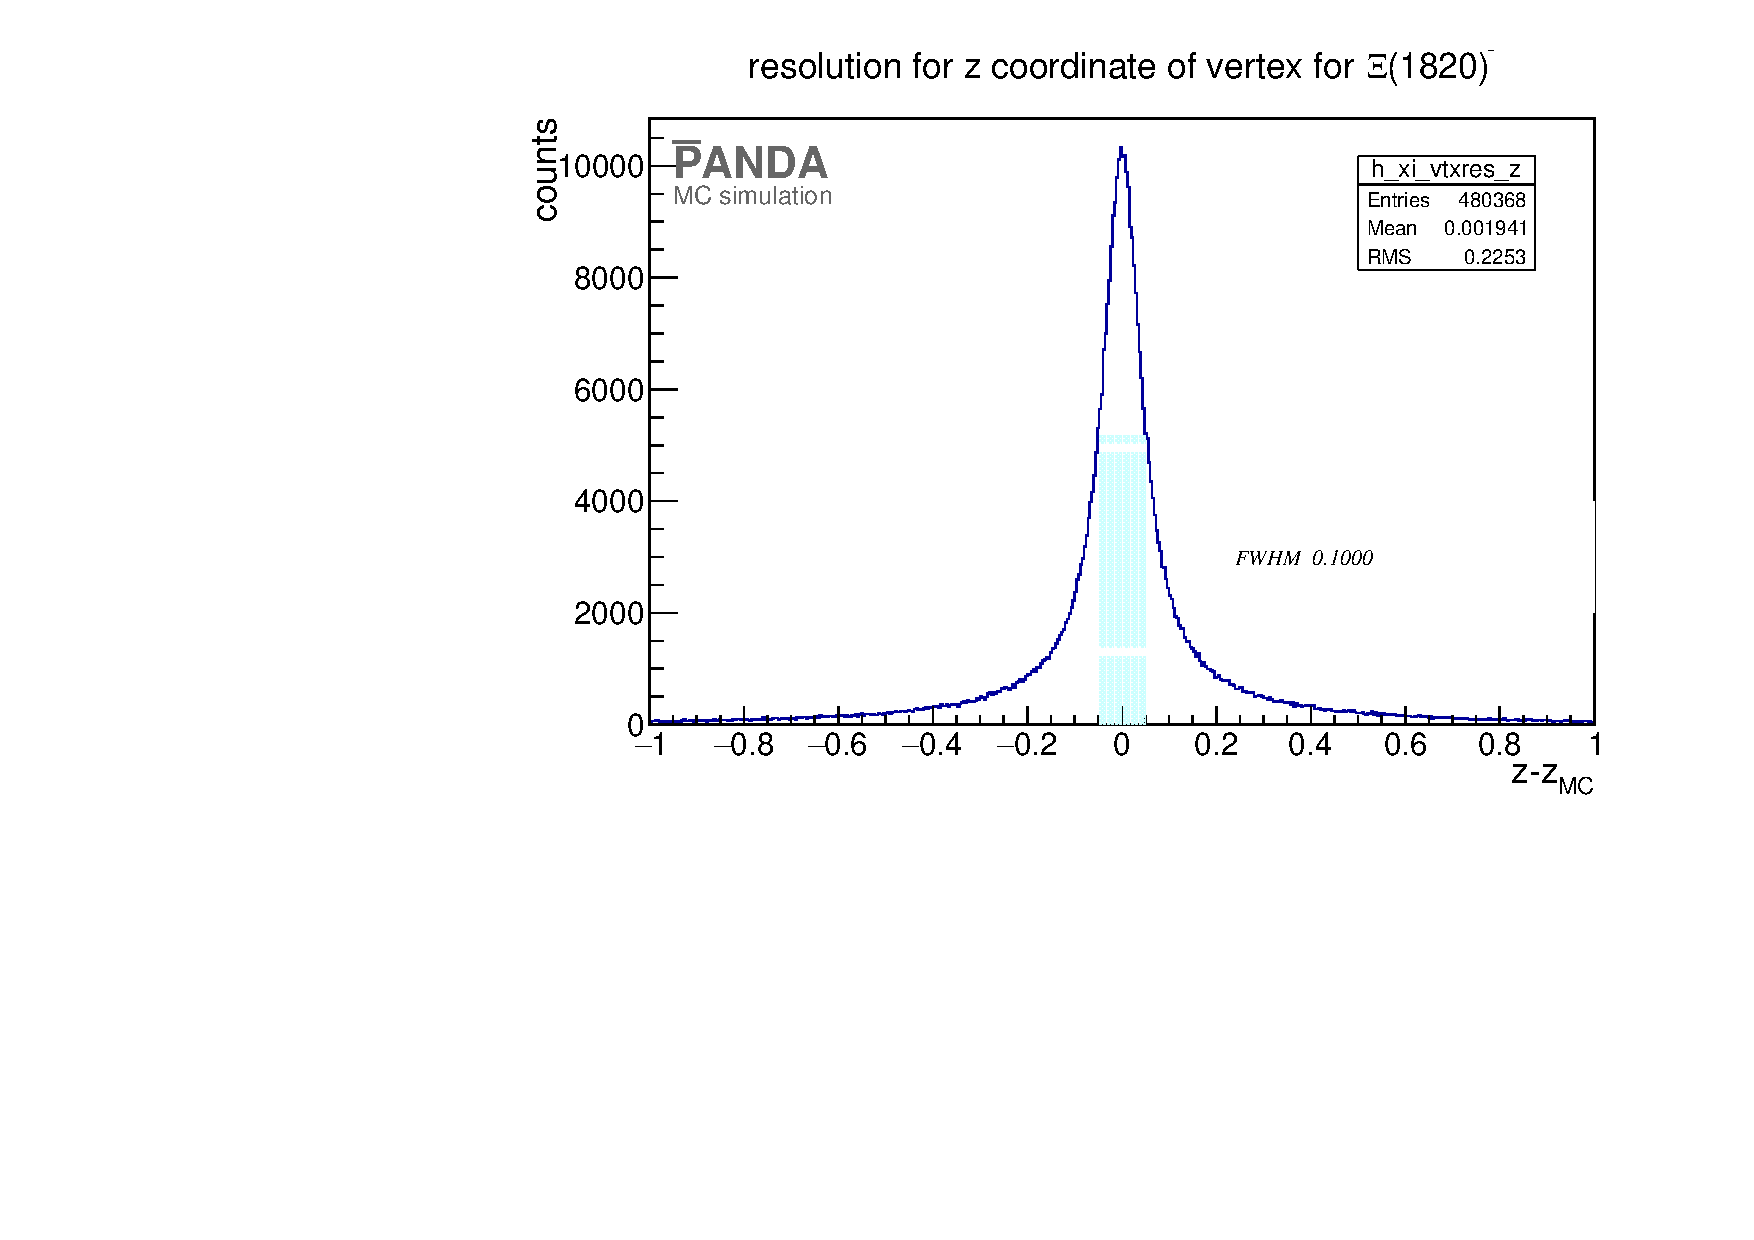
\includegraphics[width=0.49\textwidth]{./plots/Xi1820/XiMinus1820_vtxres_z.pdf}}
		\caption{Figure a) shows the vertex resolution for the y coordinate and figure b) for the z coordinate of \excitedcascade}
		\label{fig:Xi1820_vtxyz}
	\end{figure}
	
	After performing the both fits and cut on the probability values, the mass for \excitedcascade and \excitedanticascade
	can be determined by fitting the mass with a double Gaussian fit. 
	Figure \ref{fig:xi1820_mass_diffcuts} shows the mass distribution for both particles after each cut.
	
	\begin{figure}
		\centering
		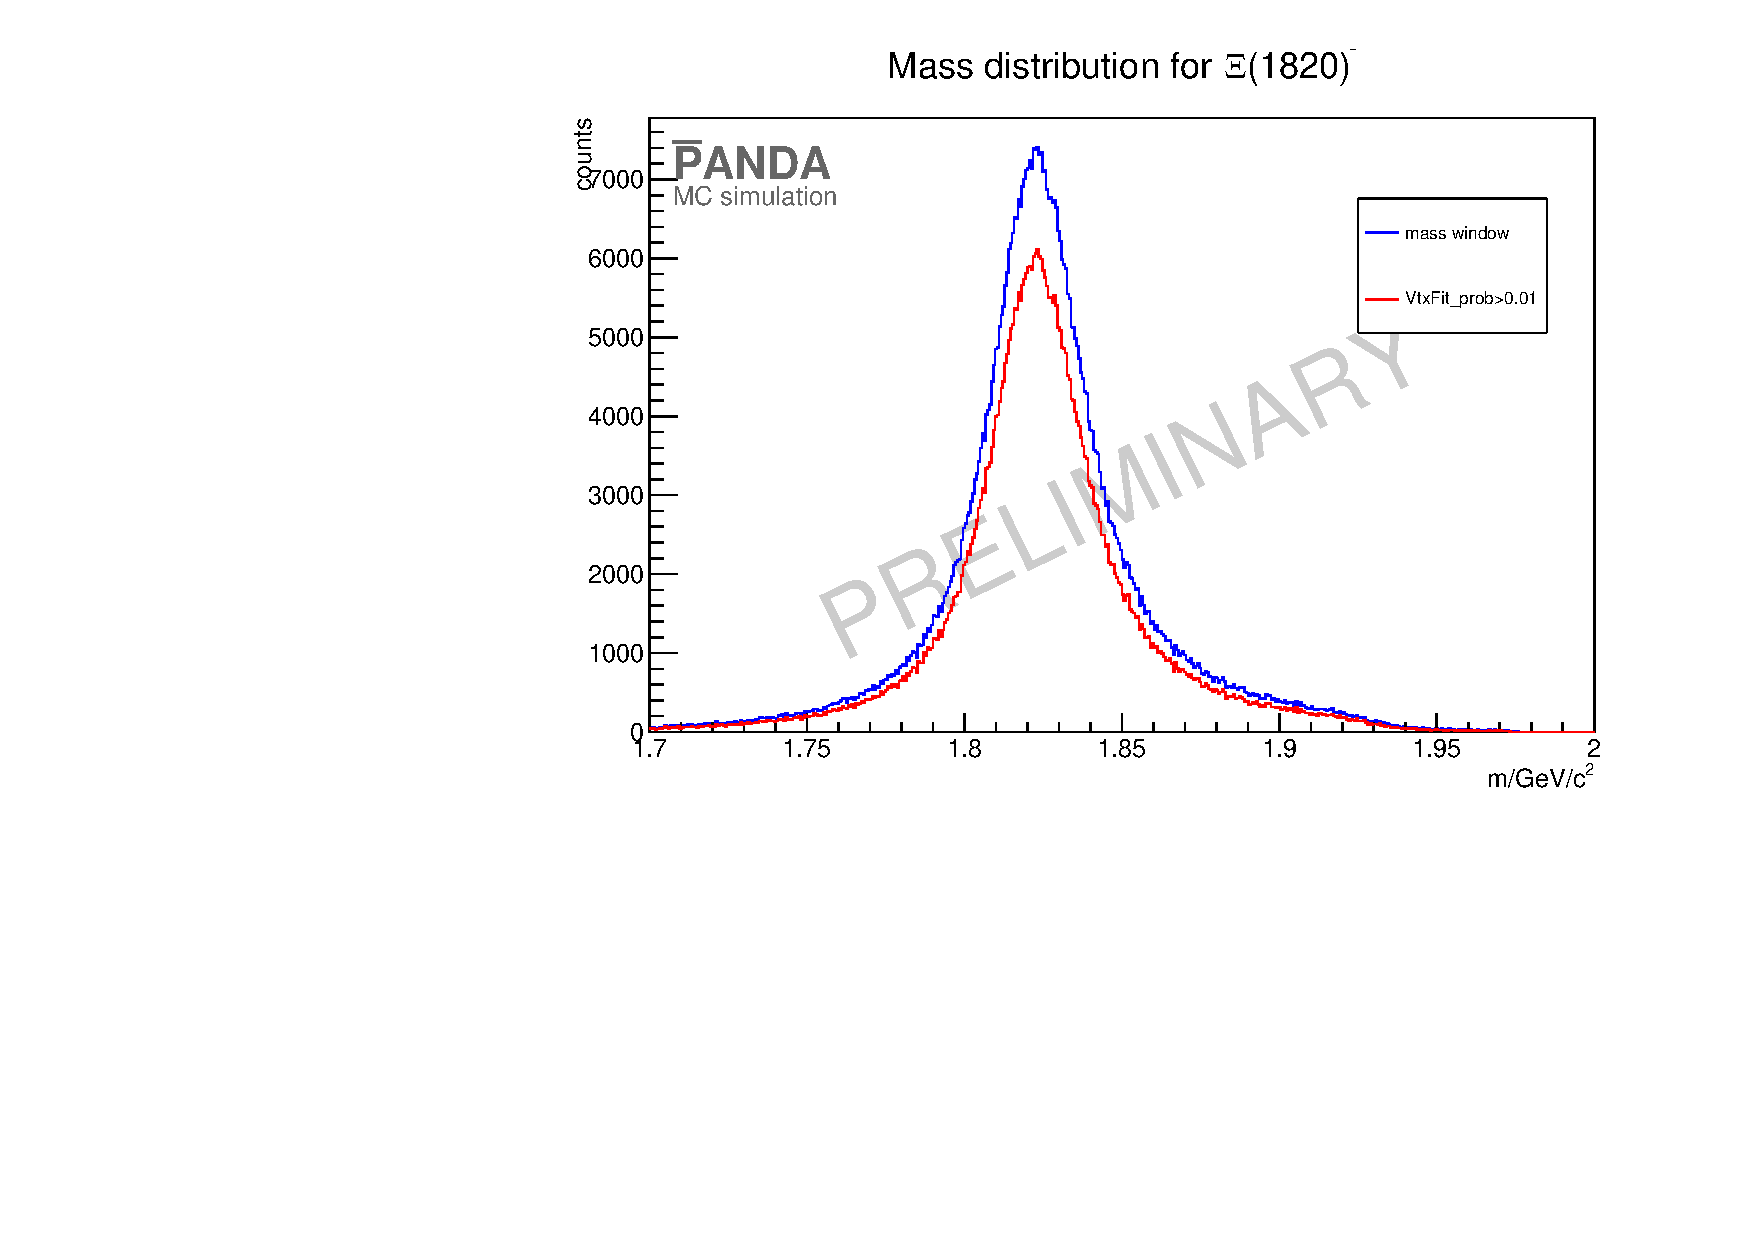
\includegraphics[width=1.\textwidth]{./plots/Xi1820/XiMinus1820_m_diffcuts.pdf}
		\caption{Mass distribution for \excitedcascade for the different cuts}
		\label{fig:xi1820_mass_diffcuts}
	
	\end{figure}
	The mass fit is exemplarily shown for the \excitedcascade in figure \ref{fig:xi1820_massfit}. 
	
	\begin{figure}
		\centering
		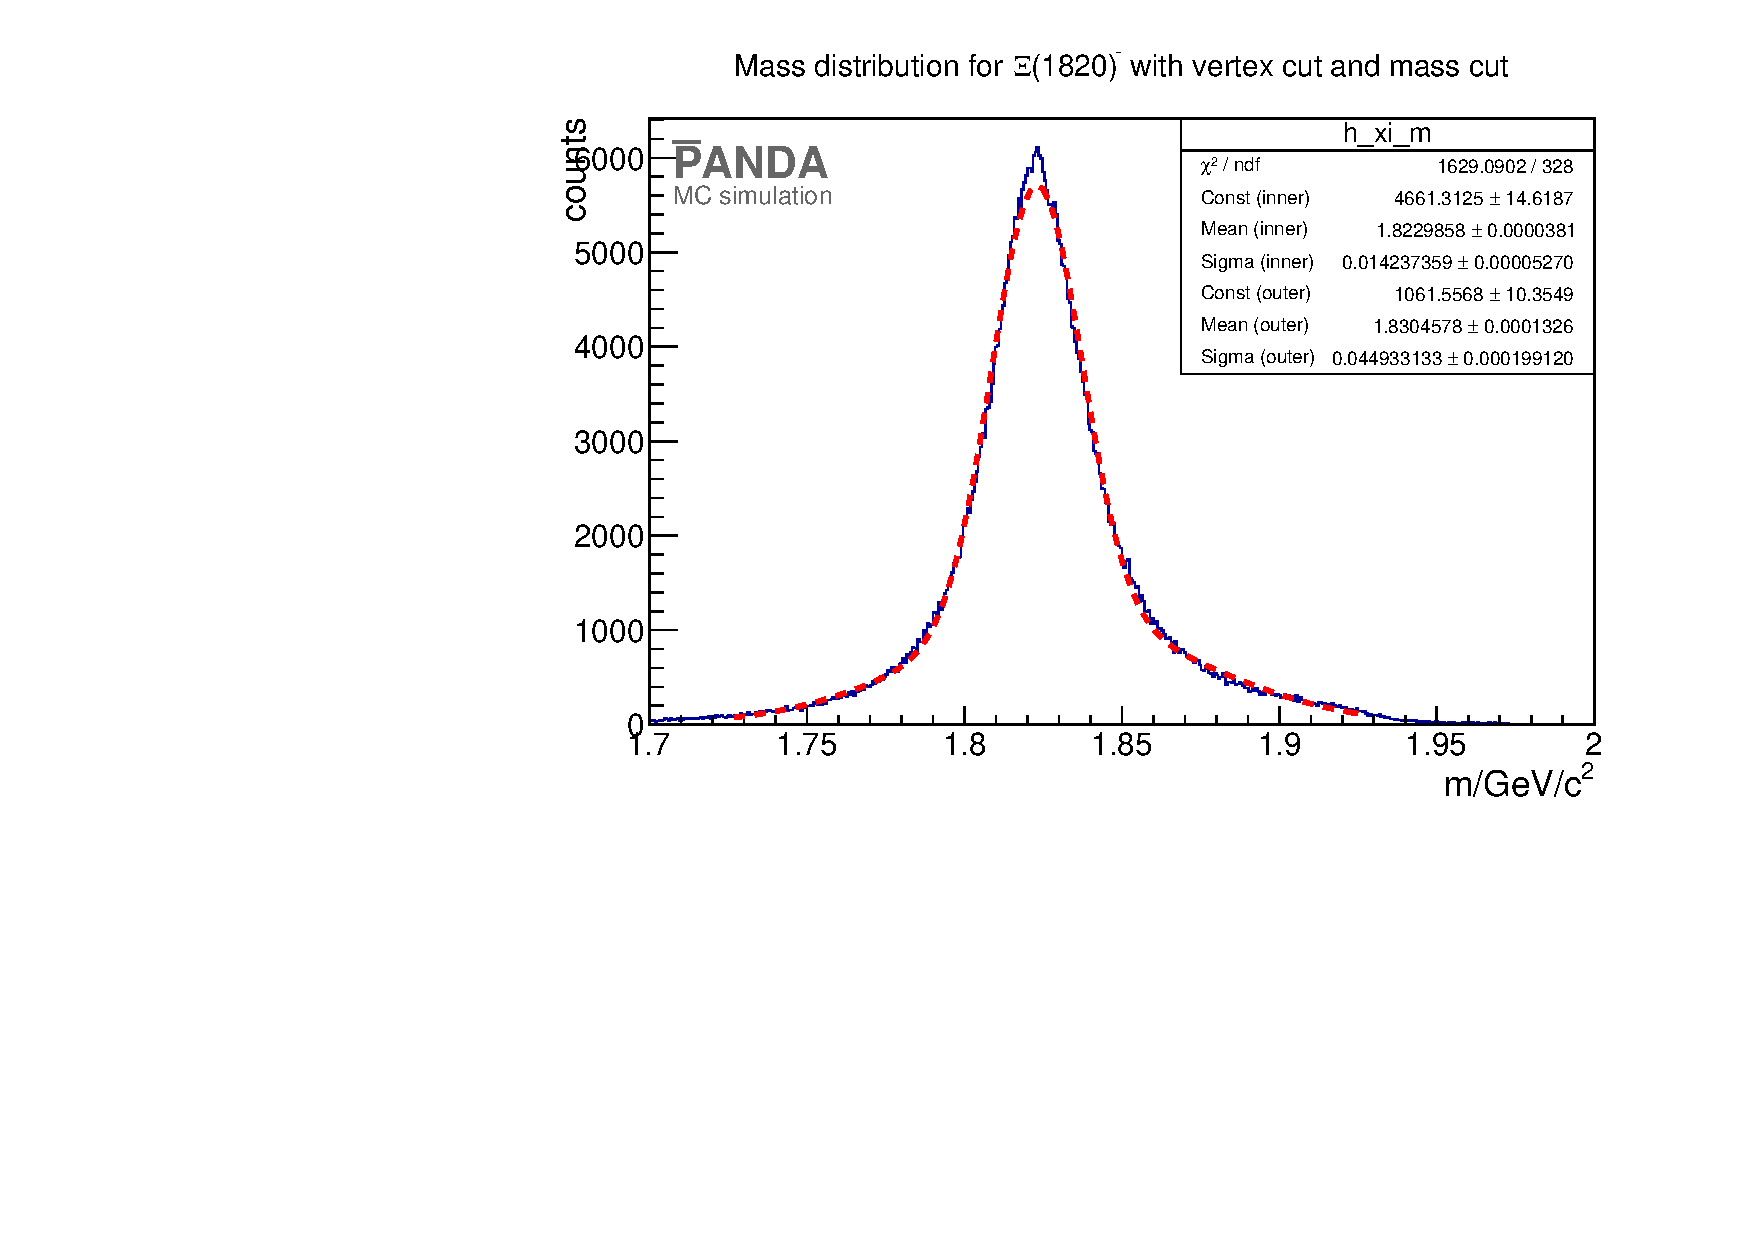
\includegraphics[width=1.\textwidth]{./plots/Xi1820/XiMinus1820_m_masscut.pdf}
		\caption{Mass distribution after all cuts for \excitedcascade.}
		\label{fig:xi1820_massfit}
	\end{figure}
	The mass values for the \excitedcascade is fitted to $1 \pm 1$\massunit and for \excitedanticascade to $1 \pm 1 $\massunit.
	These values are close to the input value.
	Figure \ref{fig:xi1820_pt_vs_pz} shows the two dimensional momentum distribution. For both subplots the x axis shows the longitudinal momentum
	and on the y axis there is shown the transverse momentum.
	
	\begin{figure}
		\centering
		\subfigure[\excitedcascade]{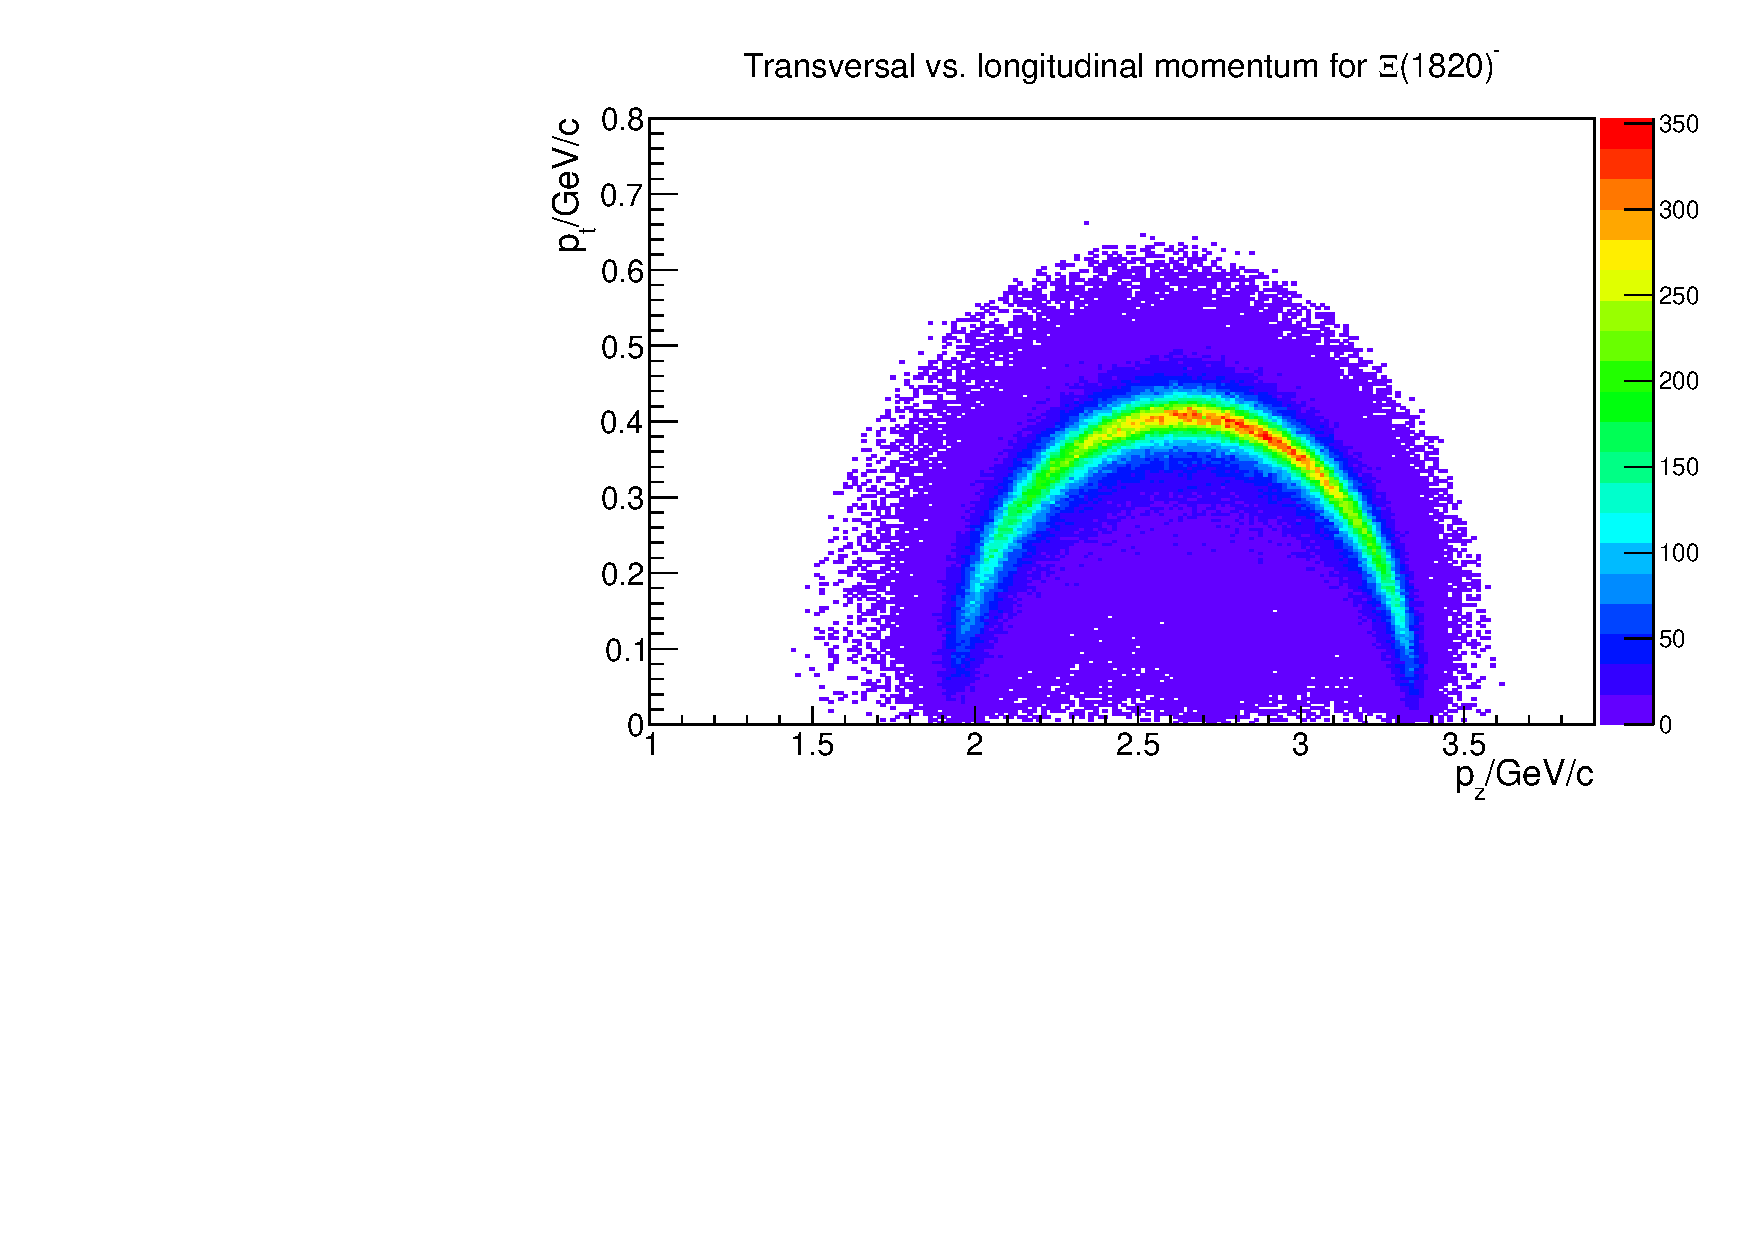
\includegraphics[width=0.49\textwidth]{./plots/Xi1820/XiMinus1820_pt_vs_pz_cut.pdf}}
		\subfigure[\excitedanticascade]{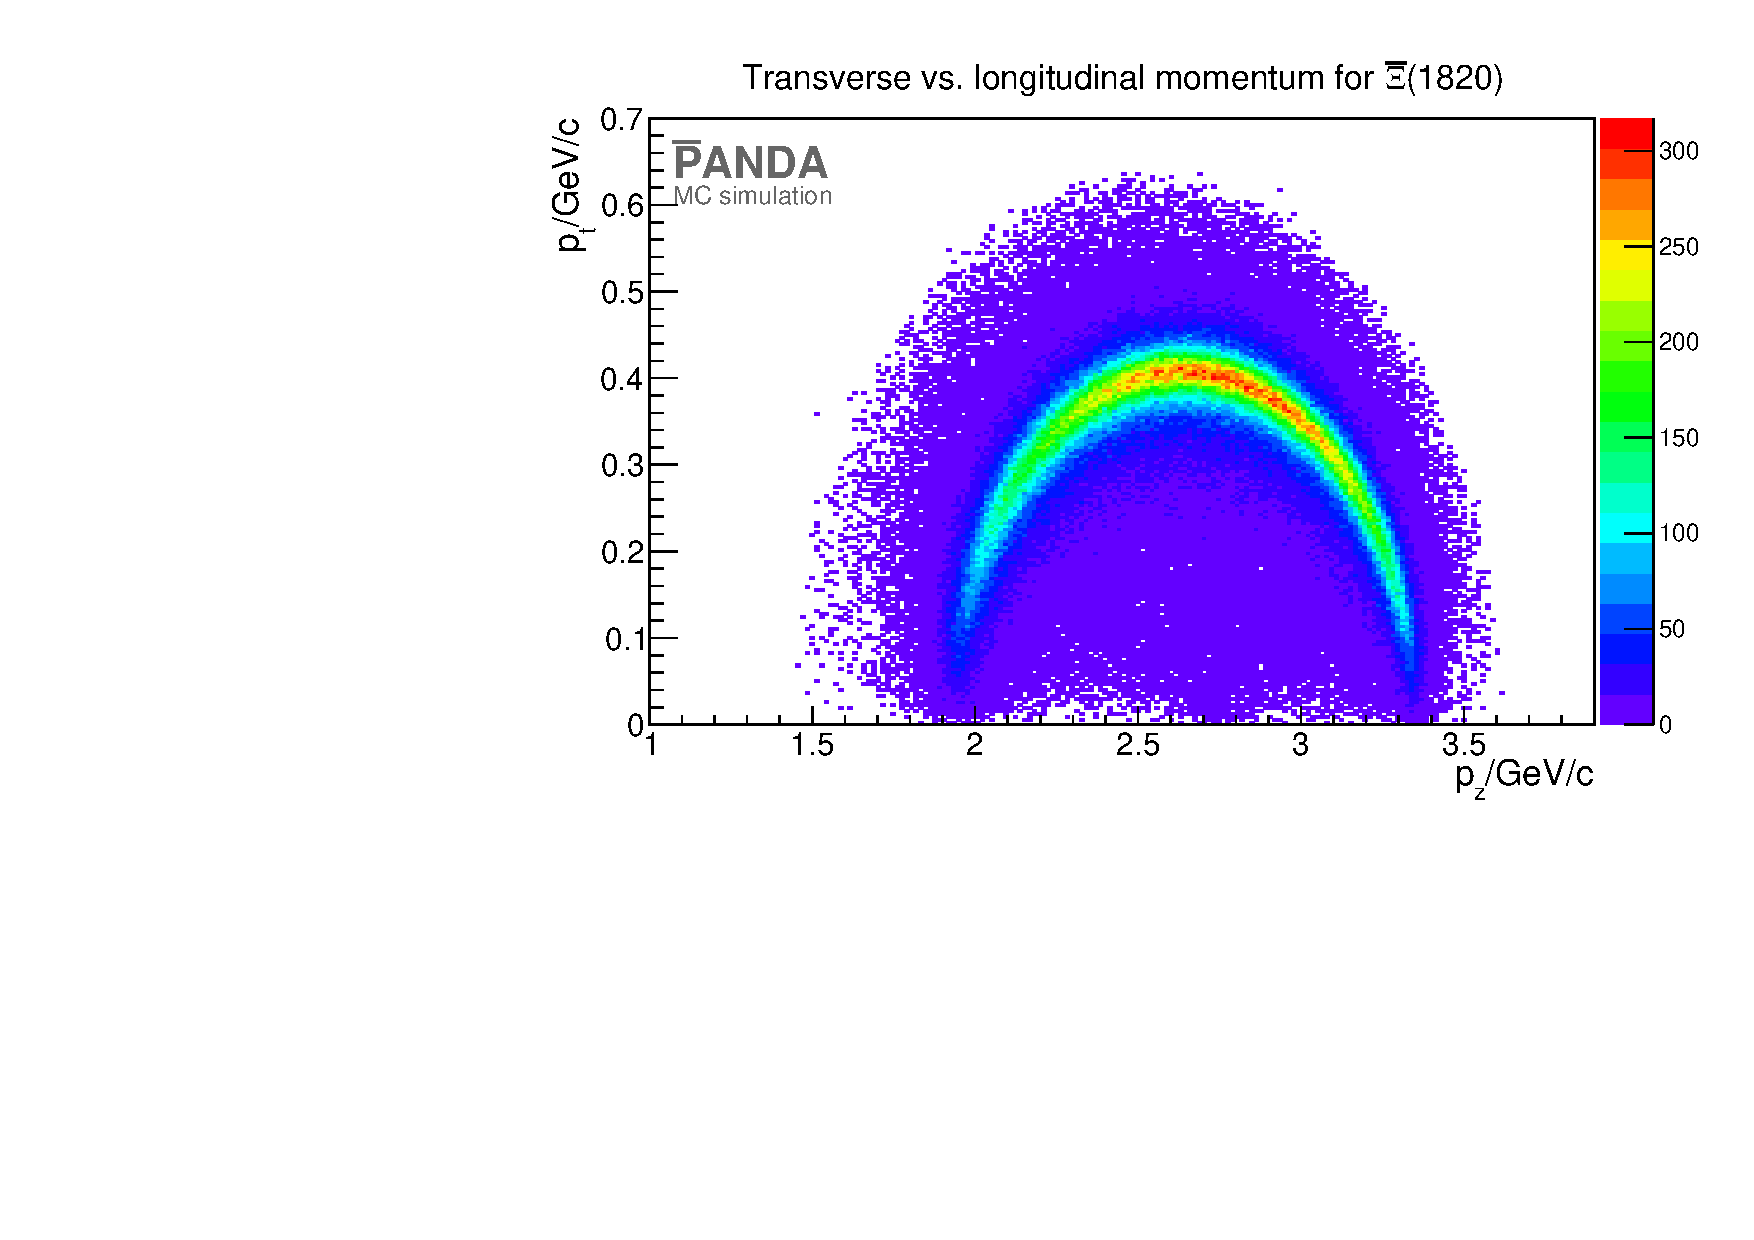
\includegraphics[width=0.49\textwidth]{./plots/Xi1820/XiPlus1820_pt_vs_pz_cut.pdf}}
		\caption{Both plots show the longitudinal versus the transverse momentum of the excited cascade baryon.}
		\label{fig:xi1820_pt_vs_pz}
	\end{figure}
	
	The reconstructed distributions are in good agreement with the distribution comming from the simulated events which are 
	shown in figure \ref{fig:MC_xi_pt_vs_pz} (b).
	
\section{Reconstruction of hole chain}

	\subsection*{Selection}
	
	To reconstruct the hole reaction chain \excitedcascade and \anticascade are combined.
	This is also done with \excitedanticascade and \cascade for the charge conjugated channel.
	For the event selection now it is use a excluding method. 
	The four momentum vector of the daughter particles is fitted to the initial for momentum vector  

	\begin{center}
		\begin{equation}\nonumber
			\left(\mt{p}_x,\, \mt{p}_y,\, \mt{p}_z,\, \mt{E} \right) = \left(0,\, 0,\, 4.6,\, 5.63 \right)
		\end{equation}
	\end{center}
	of the \pbarpSystem.	
	This fit is performed with the PndKinFitter.
	After the four momentum fit there were only those candidates selected which have a \chisq probability of more than $1\%$.
	The \chisq probablitity is shown in figure \ref{fig:xisys_prob}. 
	The red line denotes the cut value.

	\begin{figure}
		\centering
		%\includegraphics
		\caption{4-constraint fit probability}
		\label{fig:xisys_prob}
	\end{figure}
	
	The selection scheme is shown in figure \ref{fig:fourconstraintfit}
	 
	\begin{figure}
		\centering
			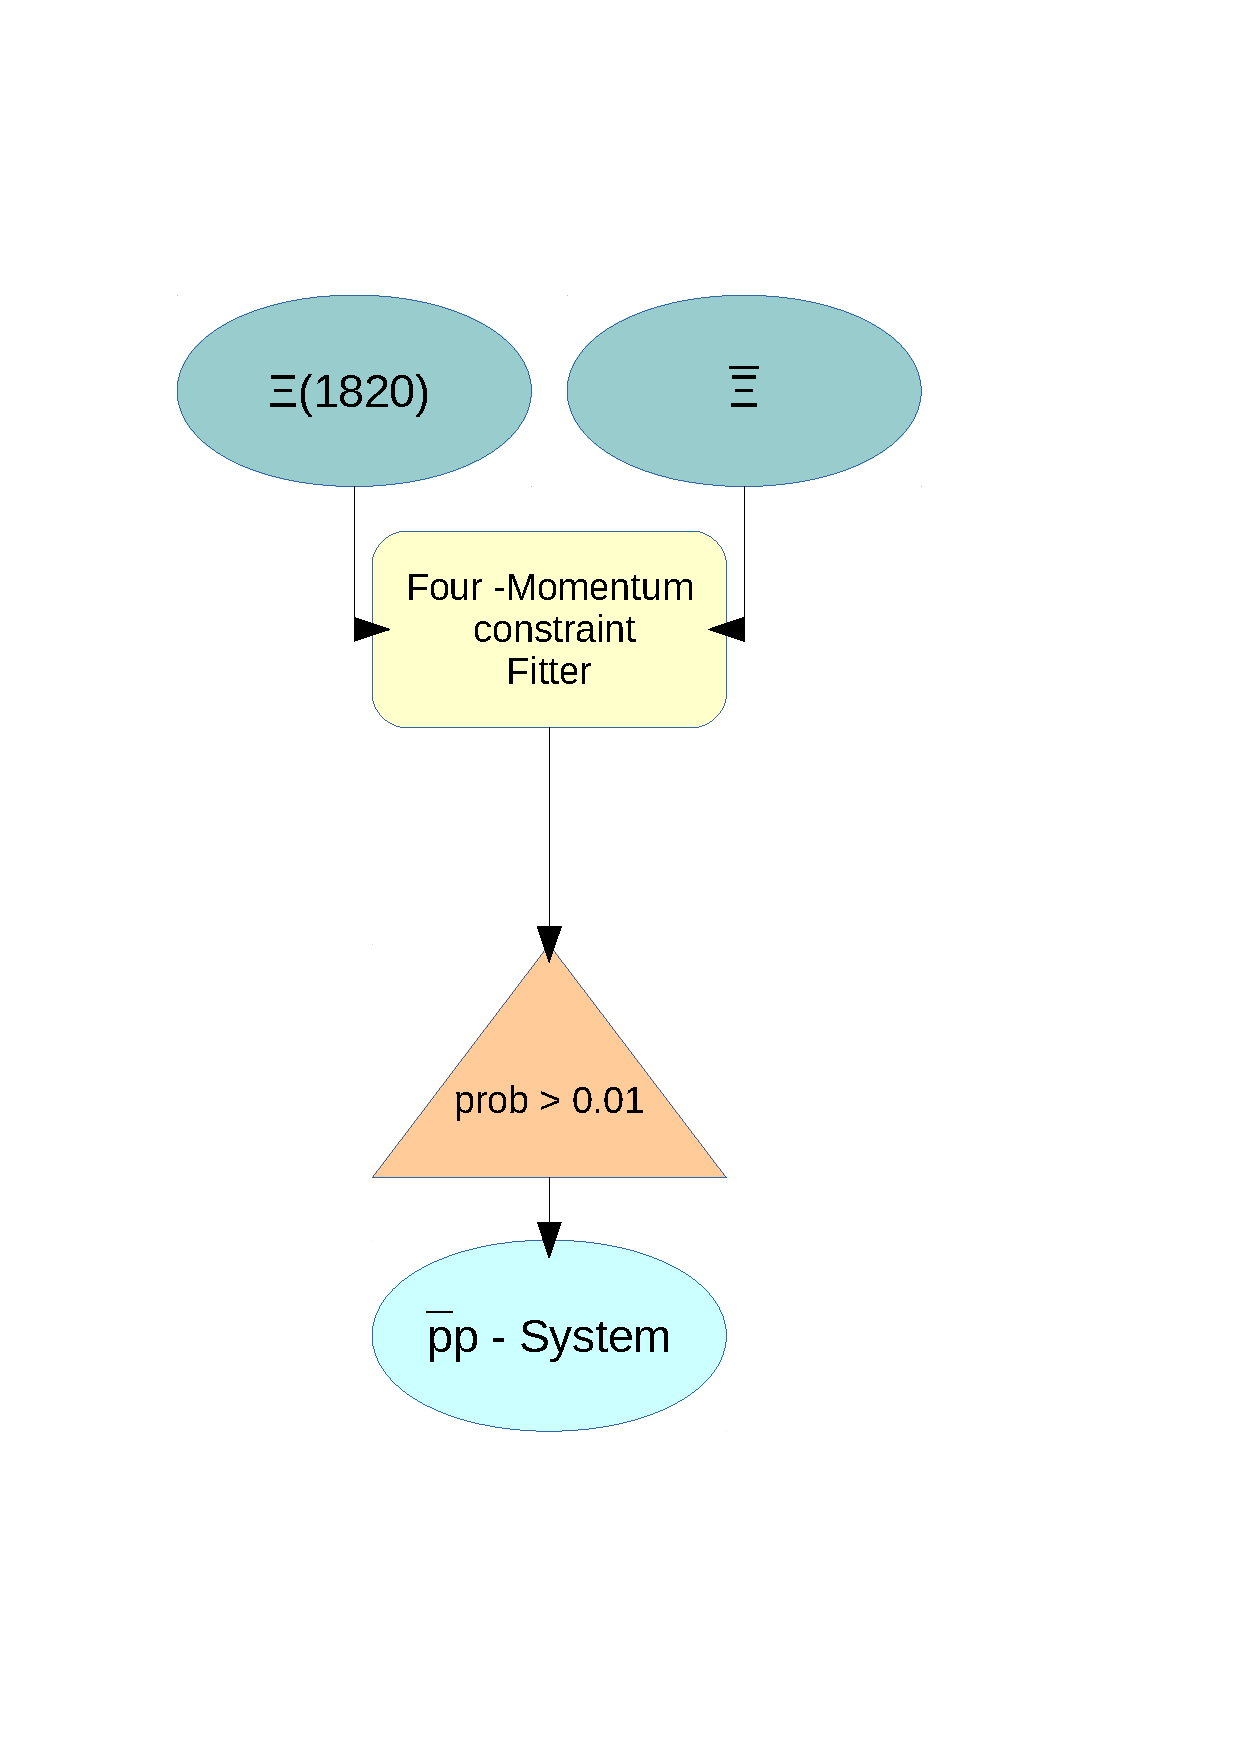
\includegraphics[width=0.50\textwidth]{./plots/combineCascadeSys.pdf}
		\caption{Scheme for 4-Constraint Fit}
		\label{fig:fourconstraintfit}
	\end{figure}
	
	\subsection*{Results}
	
	The results of the reconstruction efficiency for all non-final state particles is shown in table \ref{tab:non-finalstate_efficiency}
	and tabel \ref{tab:non-finalstate_efficiency_cc}.
	
	\begin{table}
		\centering
		\caption{reconstruction efficiency for non-final state particles for \pbarpSystem $\rightarrow$ \excitedcascade \anticascade}
		\label{tab:non-finalstate_efficiency}
		
		\begin{tabular}{lcc}
		
			\hline
			particle & reco efficiency in $\%$ & dp/p in $\%$ \\\hline
			\hline
			\lam & 50.3278&   1.50497 \\
			\alam & 41.4625&   1.45024\\
			\anticascade & 18.389&   1.2889\\
			\excitedcascade & 32.0245&   2.67691 \\
			\excitedcascade \anticascade system & 4.69293&   1.03214\\\hline
			 	
		\end{tabular}
	\end{table}
	
		\begin{table}
		\centering
		\caption{reconstruction efficiency for non-final state particles for \pbarpSystem $\rightarrow$ \excitedanticascade \cascade}
		\label{tab:non-finalstate_efficiency_cc}
		
		\begin{tabular}{lcc}
		
			\hline
			particle & reco efficiency in $\%$ & dp/p in $\%$ \\\hline
			\hline
			\lam & 42.4693&   1.45429 \\
			\alam & 48.9991&   1.50196\\
			\cascade & 18.6405&   2.29877\\
			\excitedanticascade & 33.2238&   1.31081\\
			\excitedanticascade \cascade system & 4.87227&   1.03127\\\hline
			 	
		\end{tabular}
	\end{table}
	
	How good the reconstruction works is shown in figure \ref{fig:reco_dalitzplot}.
	This plot shows the dalitz plot for the \anticascade, \lam and \kminus final states after the reconstruction. 
	Compared with the dalitz plot of the simulated particles which is shown in figure \ref{fig:eventgeneration_dalitz} the reconstruction seems to be good.
	
	\begin{figure}
		\centering
		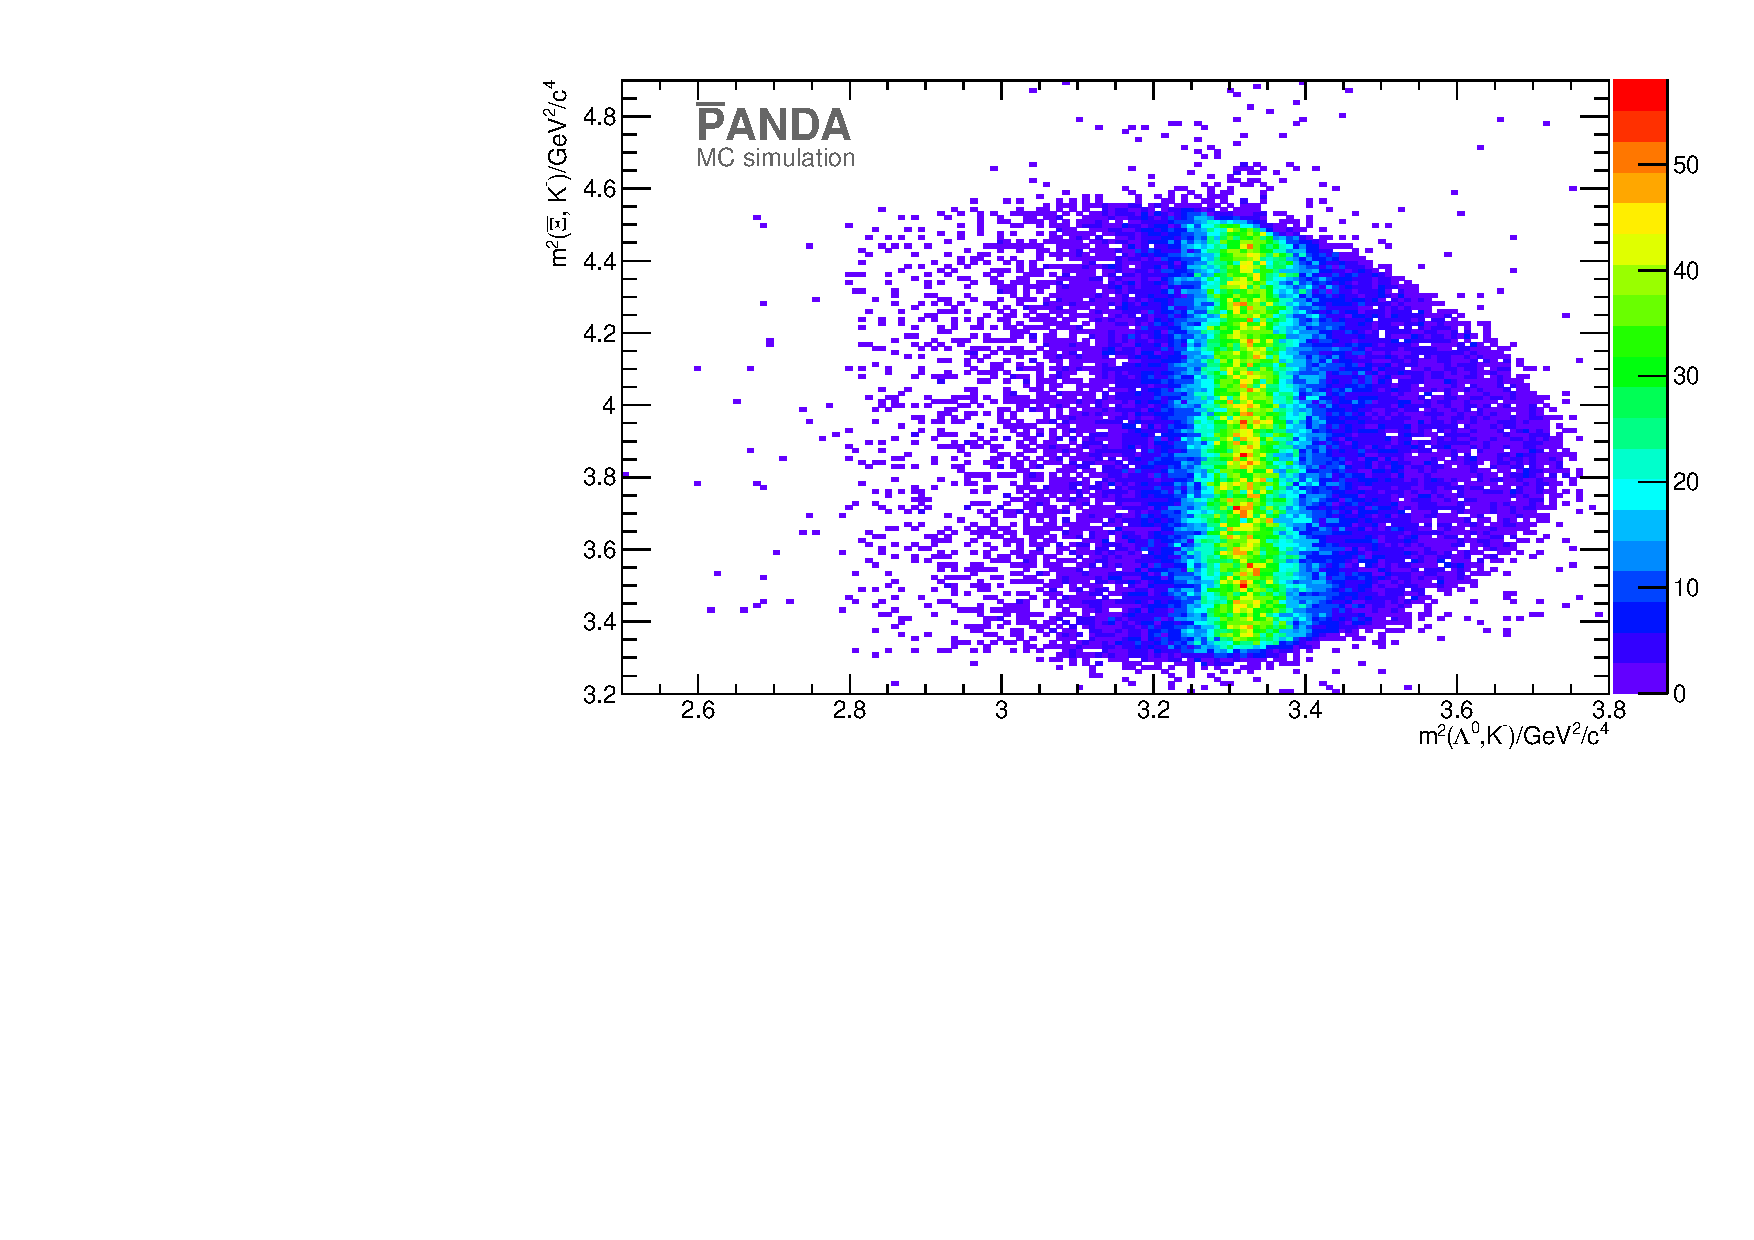
\includegraphics[width=0.8\textwidth]{./plots/pbarp/Dalitzplot_reco.pdf}
		\caption{Dalitz plot for reconstructed particles}
		\label{fig:reco_dalitzplot}
	
	\end{figure}
	
	